\documentclass[a4paper,12pt]{article}
\usepackage[utf8]{inputenc}
\usepackage{geometry}
\geometry{
 a4paper,
 left=1.25in,
 right=1.25in,
 top=1in,
 }
\usepackage[croatian,english]{babel}    %za hrvatske naslove
\usepackage[nottoc]{tocbibind}  %za pravilan table of content
\usepackage{graphicx}   %za dodavanje slika
\usepackage{amsmath}    %za matematičke forumele
\usepackage{subcaption} %za dvije slike u jednoj
\usepackage{booktabs}   %za bolje tablice
\usepackage{cite}
\usepackage{url}       %za URL linkove u bibliografiji
\usepackage{float}
\usepackage{hyperref}  %za hiperlinkove - mora biti zadnji

% Konfiguracija hyperref-a za boje i stil linkova
\hypersetup{
    colorlinks=true,        % linkovi su obojeni umjesto u okvirima
    linkcolor=black,         % boja unutarnjih linkova (TOC, reference)
    citecolor=black,        % boja citata
    urlcolor=blue,          % boja URL linkova
    filecolor=magenta,      % boja linkova na datoteke
    menucolor=red,          % boja linkova na meni
    breaklinks=true,        % dozvoljava lomljenje linkova preko redaka
    % bookmarks=true,       % stvara PDF bookmarks (default je true)
    % bookmarksopen=true,   % otvara bookmark panel
    % pdfstartview=FitH,    % kako se PDF otvara
    % pdftitle={Naslov rada},    % naslov PDF-a
    % pdfauthor={Vaše ime},      % autor PDF-a
    % pdfsubject={Tema rada},    % tema PDF-a
}

\begin{document}

\begin{center}
SVEUČILIŠTE JURJA DOBRILE U PULI 

FAKULTET INFORMATIKE

\vspace{45mm} 

\textbf{Ime Prezime}

\vspace{20mm} 

\textbf{Naslov rad}

\vspace{5mm}
DIPLOMSKI/ZAVRSNI RAD

\vfill

%Upisat tocan mjesec i godinu
Pula, svibanj, 2022. godine
\end{center}

\pagenumbering{gobble}
\clearpage
\newpage

\begin{center}
SVEUČILIŠTE JURJA DOBRILE U PULI 

FAKULTET INFORMATIKE

\vspace{45mm} 

\textbf{Tin Pritišanac}

\vspace{20mm} 

\textbf{Strategije iscrtavanja web aplikacija
    kroz različite programske okvire}

\vspace{5mm}
ZAVRŠNI RAD

\end{center}

\vspace{45mm}

\textbf{JMBAG: 0171256219, izvanredni student}

\textbf{Studijski smjer: Informatika}
\bigskip

\textbf{Kolegij: \textbf{Web aplikacije} }

\textbf{Znanstveno područje : Društvene znanosti}

\textbf{Znanstveno polje : Informacijske i komunikacijske znanosti}

\textbf{Znanstvena grana : Informacijski sustavi i informatologija}
\bigskip

\textbf{Mentor: doc. dr. sc. Nikola Tanković}

\vfill

\begin{center}

%Upisat tocan mjesec i godinu
Pula, rujan, 2025. godine

\end{center}
\pagenumbering{gobble}
\clearpage
\newpage

%Resetirat margine
\restoregeometry

\selectlanguage{croatian}
\begin{abstract}

Odabir optimalne strategije iscrtavanja web aplikacije (CSR, SSR, SSG, ISR) ključan je za postizanje dobrih performansi i korisničkog iskustva. Ovaj rad usporedno analizira navedene strategije u tri popularna programska okvira za izradu web aplikacija Next.js, Nuxt.js i SvelteKit. U svakom od programskih okvira implementirana je identična demo aplikacija sa stranicama statičnog i dinamičnog sadržaja, te su nad njima vršeni testovi ključnih metrika performansi prikupljeni Lighthouse CLI alatom u kontroliranim mrežnim uvjetima. Rezultati prikazuju prednosti i mane svake strategije iscrtavanja ovisno o tipu stranica, te koji programski okviri postižu najbolje performanse u kojim strategijama iscrtavanja.

\end{abstract}
\begin{small}
\textbf{Ključne riječi} : CSR, SSR, SSG, ISR, Next.js, Nuxt.js, SvelteKit, performanse
\end{small}

\bigskip

\selectlanguage{english}
\begin{abstract}

Selecting the optimal rendering strategy for a web application (CSR, SSR, SSG, ISR) is crucial for achieving good performance and user experience. This paper provides a comparative analysis of these strategies across three popular web application frameworks: Next.js, Nuxt.js, and SvelteKit. An identical demo application containing both static and dynamic content pages was implemented in each framework, and key performance metrics were tested using the Lighthouse CLI tool under controlled network conditions. The results highlight the advantages and disadvantages of each rendering strategy depending on the page type, as well as which frameworks achieve the best performance under specific rendering strategies.

\end{abstract}
\begin{small}
\textbf{Keywords} : CSR, SSR, SSG, ISR, Next.js, Nuxt.js, SvelteKit, performance
\end{small}

\pagenumbering{gobble}
\clearpage
\newpage

\selectlanguage{croatian}
\tableofcontents
\pagenumbering{gobble}
\clearpage
\newpage

\pagenumbering{arabic}

\section{Uvod}

U današnjem okruženju razvoja web aplikacija, više nego ikada prije, vidljiva je težnja i potreba industrije dolazi  za postizanjem boljih performansi, skalabilnosti i korisničkog iskustva. Ta potreba potaknula je istraživanje i razvoj novih rješenja kao odgovor na pitanje kako najoptimalnije i najbrže dostaviti web sadržaj korisniku? Kritična stavka u odgovoru na ovo pitanje je upravo odabir odgovarajuće strategije iscrtavanja web aplikacija s obzirom na vrstu sadržaja koji se korisniku servira. Web aplikacije uvelike su evoluirale od starog pristupa serviranja statičnih stranica do današnjih vrlo interaktivnih dinamičnih aplikacija koje zahtijevaju sofisticirane pristupe dostavljanja i prikazivanja sadržaja krajnjem korisniku. \cite{moore2024rendering} Tradicionalne metode iscrtavanja poput iscrtavanja na serveru (SSR) gdje se svježi sadržaj generira na svaki zahtjev korisnika i generiranja statičnih stranica (SSG) kod koje se svaka stranica unaprijed iscrtava u statičnu datoteku već duže vrijeme čine temelj i osnovni standard u razvoju web aplikacija. Povećanje kompleksnosti aplikacija i potreba za sve višim performansama izrodili su i nove hibridne metode iscrtavanja poput inkrementalne statičke generacije (ISR).

\bigskip

Svaka od ovih metoda ima specifične prednosti i nedostatke koji se odražavaju na metrike poput početnog vremena učitavanja sadržaja, razine interaktivnosti, optimizacije za tražilice (SEO) i dr. Odabir strategije iscrtavanja uvelike utječe na percepciju krajnjeg korisnika, troškove infrastrukture te kompleksnost u razvoju i arhitekturi aplikacije.

\bigskip

Popularni programski okviri za razvoj web aplikacija kao što su Next.js, Nuxt i SvelteKit podržavaju većinu novih strategija iscrtavanja čime otvaraju programerima mnoge mogućnosti za optimiziranje procesa dostave sadržaja korisniku.

\bigskip

Pri odabiru programskog okvira uzimaju se u obzir mnogi faktori, a jedan od njih su i performanse, koje direktno utječu na korisničko iskustvo pogotovo u ograničenim mrežnim uvjetima.
U ovom radu provedena je usporedna analiza performansi sva tri programska okvira u svakoj od  četiri odabrane strategije iscrtavanja (CSR, SSR, SSG i ISR). Postavljeni ciljevi su:

\begin{enumerate}
    \item Izrada i implementacija funkcionalno i stilski identične web aplikacije sa pod stranicama dinamičnog i statičnog sadržaja (blog).
    \item Sustavno mjerenje i usporedba odabranih metrika performansi što uključuje: vrijeme do prvog bajta (TTFB), prvo iscrtavanje sadržaja (FCP), iscrtavanje najvećeg sadržaja (LCP), ukupno vrijeme blokiranja (TBT), vrijeme do interaktivnosti (TTI), veličinu paketa (bundle size) i vremena izgradnje (build time) nad svakom kombinacijom programskog okvira i strategije iscrtavanja te na sve 3 definirane pod stranice.
    \item Utvrđivanje prednosti i nedostataka svake strategije iscrtavanja unutar svakog programskog okvira analizom prikupljenih podataka
    \item Na temelju rezultata analize donijeti zaključke o tome koji programski okvir nudi najbolje performanse s obzirom na odabranu strategiju iscrtavanja.
\end{enumerate}

Kako bi rezultati bili reprezentativni i usporedivi sa stvarnim korisničkim iskustvom, sva mjerenja izmjerena su u stvarnim uvjetima na aplikacijama postavljenima na platformi Vercel, koja u trenutku pisanja ovog rada jedina nudi mogućnost postavljanja sve četiri strategije iscrtavanja u svim navedenim programskim okvirima. Za testiranje je osigurana stabilna i brza internetska veza prema Internetu, no sami testovi provedeni su uz postavljena ograničenja kako bi se jasnije istaknule razlike u performansama. Odabrano je ograničenje veze koje simulira sporu 4G vezu te dvostruko smanjenje brzine procesora.

\bigskip

Ovo istraživanje nastoji pružiti bolji uvid u trenutne mogućnosti iscrtavanja koje su dostupne web developerima, te im time pomoći u donošenju boljih odluka pri odabiru programskog okvira i strategije iscrtavanja za svoju web aplikaciju. Prvi dio rada baviti će se pregledom najpopularnijih strategija iscrtavanja i programskih okvira, a drugi dio prezentacijom i analizom dobivenih rezultata, raspravom te zaključnim razmatranjima.

\subsection{Strategije iscrtavanja}

Pojam strategije iscrtavanja odnosi se na proces pretvaranja koda u vizualni sadržaj koji korisnik može vidjeti i s kojim može vršiti interakciju kroz web preglednik. \cite{moore2024rendering} Ovaj proces utječe na korisničko iskustvo određujući koliko brzo će se sadržaj učitati korisniku i koliko će aplikacija biti prilagodljiva i dinamična.
Odabir strategije iscrtavanja također bitno utječe i na SEO tj. vidljivost kod pretraživanja internetskim tražilicama. \cite{bratslavsky2025rendering}

\bigskip

Moderne SPA aplikacije najčešće  podržavanju različite strategije iscrtavanja, a određene platforme poput Vercela i
Netlifyja pružaju dodatnu podršku popularnim programskim okvirima, olakšavajući njihovu konfiguraciju i integraciju. Slijedi kratak pregled strategija iscrtavanja obrađenih u ovom radu.

\subsubsection{Iscrtavanje na strani klijenta (CSR)}

Ova metoda iscrtavanja nastala je još početkom 21. stoljeća razvojem programskih okvira poput AngularJS-a, Reacta i Vuea kada je nastao veliki prijelaz u industriji sa monolitne web arhitekture na tzv. jednostranične aplikacije (SPA) koje se za ažuriranje sučelja, navigaciju i dohvaćanje podataka oslanjaju na JavaScript kod koji se izvršava u pregledniku.

\bigskip

Kod ove strategije iscrtavanja, na klijent se šalje jedan prazan HTML dokument, zajedno sa svim drugim resursima (CSS i JavaScript paketi). Umjesto da je sav sadržaj već unesen u HTML dokument i odmah spreman za iscrtavanje u pregledniku, preglednik najprije mora pričekati da se preuzme sav potreban JavaScript kod, te se njegovim izvršavanjem HTML dokument ispunjava elementima koji će se iscrtati. Kod navigacije između stranica, ne dolazi do dohvaćanja novog HTML dokumenta, već JavaScript ažurira postojeći HTML novim sadržajem oslanjajući se na AJAX i XML. Time se izbjegavaju ponovna učitavanja koja usporavaju rad aplikacije i štede mrežne resurse. \cite{beran2023usporedba}

\bigskip

\textbf{Prednosti ove strategije su:}

\begin{itemize}
    \item Responzivnost i interaktivnost – promjene na stranici vidljive su odmah, nema potrebe za dohvaćanjem nove stranice prilikom navigacije.
    \item Ušteda resursa poslužitelja – umjesto dohvaćanja cijelog novog HTML dokumenta za svaku stranicu, dohvaća se samo onaj dio podataka koji je potreban (najčešće u JSON formatu)
    \item Mogućnost korištenja aplikacije kada mrežna veza nije dostupna (offline) – ovakva funkcionalnost postiže se pametnim predmemoriranjem (engl. caching).
    \item Uvijek svježi podaci – budući da stranice nisu prethodno statički generirane, osigurava se svježina prikazanih podataka.
\end{itemize}

\bigskip

\textbf{Nedostaci ove strategije su:}

\begin{itemize}
    \item Početna brzina učitavanja – iako je aplikacija generalno brža nakon početnog učitavanja JavaScripta, prvo učitavanje kada korisnik posjeti stranicu može biti znatno sporije zbog potrebe da se učita i izvrši sav potreban JavaScript kod prije iscrtavanja sadržaja. Ovo ograničenje posebno dolazi do izražaja prilikom učitavanja na sporijim mrežama.
    \item Lošiji SEO – iako današnji pretraživači\footnote{Eng. crawler – automatizirani robot koji tražilica koristi za istraživanje, pronalazak i indeksiranje web stranica \cite{googlesearch}} mogu očitati i stranice iscrtane ovom strategijom, primarno su optimizirani su za čitanje statičnog HTML-a. Zbog ovog nedostatka, ova se strategija se sve manje koristi za web aplikacije kod kojih je važan dobar SEO.
    \item Lošije performanse na slabijim uređajima – zbog činjenice da je potrebno najprije izvršiti JavaScript kod na strani klijenta, kod slabijih i starijih uređaja može doći do usporavanja učitavanja i pada performansi.
    \item Manjak podrške za korisnike koji nisu omogućili JavaScript u pregledniku – bez JavaScripta sadržaj stranice se ne može iscrtati.
\end{itemize}

S obzirom na navedene prednosti i nedostatke ova strategija iscrtavanja najbolja je za tipove aplikacija koje imaju slijedeća obilježja:
\begin{itemize}
    \item Potreba za visokom razinom interaktivnosti (dashboards)
    \item Gdje SEO nije bitan čimbenik (admin i korisničke stranice)
    \item Progresivne web aplikacije
    \item Potreba za smanjenjem opterećenja poslužitelja
\end{itemize}
\vfill

\subsubsection{Iscrtavanje na strani poslužitelja (SSR)}

Kako bi se uklonili nedostatci koje sa sobom nosi iscrtavanje na strani klijenta, razvila se nova popularna strategija iscrtavanja – iscrtavanje na strani poslužitelja. Ova strategija se naizgled vraća korak prema već poznatom i prvobitnom načinu iscrtavanja – iscrtavanju na poslužitelju ili serveru i višestraničnoj web aplikaciji (MPA) kakve su postojale od začetaka Interneta.

\bigskip

No moderni programski okviri poput Nuxta i SvelteKita spajaju SSR i CSR na način da se prilikom prvobitnog posjeta stranici ona iscrtava na poslužitelju, te se korisniku šalje već popunjen HTML dokument koji preglednik može odmah krenuti prikazivati, a u pozadini se događa proces zvan hidracija. Ovo je proces u kojem se učitava sav potreban JavaScript kod koji se izvršava i povezuje sa HTML elementima stranice te čini stranicu interaktivnom, slično kao kod CSR strategije. Svaki slijedeći zahtjev za navigaciju između stranica ili ažuriranje podataka događa se na strani klijenta i funkcionira kao CSR aplikacija.

\bigskip

Next.js programski okvir u novijim verzijama koristi tzv. iscrtavanje na strani poslužitelja u stvarnom vremenu (Streaming SSR). U ovom načinu rada, na serveru se postupno iscrtavaju zasebni dijelovi HTML dokumenta po redoslijedu kako podaci postaju dostupni i takav dokument se odmah šalje pregledniku na prikaz. Ovime se nastoji izbjeći nedostatak klasičnog SSR-a a to je čekanje na poslužitelj da generira cijeli HTML dokument prije nego ga pošalje klijentu.  \cite{nextjsloading}

\bigskip

Kako bi SSR strategija mogla funkcionirati, na poslužitelju je potrebno odgovarajuće okruženje koje podržava izvođenje JavaScript koda i generiranje HTML stranica. To je najčešće Node.js \cite{vuejsssr}

\bigskip

\textbf{Prednosti ove strategije su:}

\begin{itemize}
    \item Nema čekanja na učitavanje JavaScripta – budući da se na zahtjev klijenta na poslužitelju generira HTML datoteka koja mu se odmah dostavlja spremna za prikaz, nema potrebe za čekanjem na preuzimanje i izvršavanje JavaScript koda.
    \item Bolji SEO – statičke HTML datoteke popunjene sadržajem mnogo su bolje za mrežne pretraživače, koji iz njih brže i lakše dolaze do relevantnih podataka o stranici.
    \item HTML datoteka mogu se spremiti u pričuvnu memoriju preglednika, što omogućava pregled stranice i kada nema pristupa internetu.
    \item Svježina podataka – na svaki zahtjev klijenta generira se novi HTML dokument sa ažuriranim podacima.
\end{itemize}

\bigskip

\textbf{Nedostaci ove strategije su:}

\begin{itemize}
    \item Čekanje na poslužitelju – iako nema čekanja na izvršavanje JavaScript ko\-da (prije prikaza sadržaja) na strani klijenta, prilikom prve posjete stranici potrebno je pričekati na poslužitelja da izgradi HTML dokument koji nije prethodno generiran. Prethodno spomenuti streaming SSR pokušava ublažiti i ovaj nedostatak.
    \item Čekanje do interaktivnosti – unatoč brzom prikazu početnog sadržaja stranice, ipak je potrebno pričekati na proces hidracije kako bi stranica postala interaktivna. To uključuje preuzimanje JavaScript paketa i izvršavanje koda što može blokirati glavnu procesorsku nit i time povećati vrijeme do interaktivnosti (TTI).
    \item Povećano korištenje resursa poslužitelja – generiranje HTML dokumenata na svaki zahtjev korisnika rezultira i većom potrošnjom računalnih resursa poput memorije i procesorske snage, što je kod CSR-a prebačeno na klijentski uređaj.
    \item Složeniji proces razvoja – zbog činjenice da se određeni dijelovi koda mogu izvršavati samo na klijentu ili samo na poslužitelju, raste i kompleksnost u razvoju aplikacije. \cite{beran2023usporedba}
\end{itemize}

S obzirom na navedene prednosti i nedostatke ova strategija iscrtavanja najbolja je za tipove aplikacija koje imaju slijedeća obilježja:
\begin{itemize}
    \item Stalna potreba za svježim i ažuriranim podacima
    \item Visoka razina personalizacije (custom dashboards)
    \item Vizualizacija podataka u realnom vremenu
    \item Dobar SEO \cite{moore2024rendering}
\end{itemize}

\subsubsection{Generiranje statičkih stranica (SSG)}

Kod ove strategije iscrtavanja HTML stranice se unaprijed generiraju na serveru prilikom izgradnje aplikacije (engl. build time), te se zatim poslužuju klijentima na zahtjev, bez potrebe za ponovnim generiranjem na svakom zahtjevu kao kod SSR-a. Ovakve stranice se mogu i spremiti u priručnu memoriju (engl. cache) koristeći CDN radi brže distribucije korisnicima \cite{nextjsssg, sanityssg}

\bigskip
\textbf{Glavne prednosti ove strategije su: \cite{moore2024rendering}}
\begin{itemize}
    \item Najbrže moguće učitavanje stranice – budući da su stranice statični HTML, nije potrebno čekati na njihovo generiranje na poslužitelju ili na preuzimanje i izvršavanje JavaScript koda
    \item Odlične su za SEO – budući da se brzo učitavanju i sadrže sav potrebni sadržaj idealne su za pregled od strane pretraživača
    \item Nisko opterećenje poslužitelja – nema potrebe za obradom ili generiranjem HTML-a, već je spreman za slanje klijentu
    \item Najniži troškovi infrastrukture
\end{itemize}

\bigskip

\textbf{Nedostatci ove strategije su:}

\begin{itemize}
    \item Duže vrijeme izgradnje ako postoji veliki broj stranica
    \item Za ažuriranje sadržaja potrebno je ponovno inicirati izgradnju i postavljanje (build and deploy)
    \item Nije pogodno za stranice sa dinamičnim i često promjenjivim sadržajem
\end{itemize}

S obzirom na navedene prednosti i nedostatke ova strategija iscrtavanja najbolja je za stranice kod kojih se sadržaj gotovo nikada ili vrlo rijetko mijenja poput:
\begin{itemize}
    \item Marketinške stranice
    \item Blog postovi
    \item E-commerce proizvodi
    \item Dokumentacija i pomoć
\end{itemize}
Generalno pravilo je postaviti pitanje, može li se stranica generirati unaprijed, prije korisničkog zahtjeva? Ako je odgovor potvrdan, SSG se nameće kao logičan izbor. \cite{nextjsssg}

Postoji mogućnost kombiniranja SSG-a i CSR-a gdje se stranica servira sa prethodno generiranim statičnim dijelom koji se ne mijenja, a po učitavanju JavaScripta na klijentu se ispunjavaju dinamični dijelovi stranice svježim podacima. Ovo je alternativa korištenju SSR strategije, koja također ima svoje prednosti i nedostatke. \cite{nextjsssg}

\subsubsection{Inkrementalna statička generacija (ISR)}

Ovu strategija iscrtavanja neki nazivaju i hibridnim web razvojem jer kombinira generiranje statičnih stranica (SSG) sa iscrtavanjem na strani poslužitelja (SSR).

\bigskip

Funkcionira na način da se najprije generira statična stranica kojoj se odredi vrijeme revalidacije, tj. vrijeme nakon kojega će se ona smatrati zastarjelom i biti će ju potrebno ponovno  generirati. No okidač za ovu generaciju biti će zahtjev prvog posjetitelja nakon vremena isteka revalidacije. Tom posjetitelju će se odmah isporučiti ova stara verzija stranice bez obzira koliko je dugo prekoračeno njeno vrijeme validacije, te će se nakon uspješne ponovne generacije u pozadini, nova verzija stranice poslužiti prvom slijedećem klijentu. Na ovaj način novo generirana stranica se dodaje u web aplikaciju.

\bigskip

Uobičajeni način objavljivanja na poslužitelj jest atomsko objavljivanje, tj. kada se cjelokupni kod, resursi i konfiguracija ažuriraju u isto vrijeme. Ovaj način objavljivanja čuva integritet stranice i omogućava jednostavan opoziv objave i povratak na prijašnju verziju u slučaju potrebe (engl. rollback). Svaka pojedinačna objava je jedna cjelovita verzija web aplikacije. ISR strategija razbija ovaj integritet budući da stalno nadodaje novo generirane stranice u web aplikaciju, odvojeno od početno izgrađenog koda. Zbog ovog spremanja u pričuvnu memoriju (engl. caching)  je vrlo teško učiniti povratak na prethodnu verziju, a pri tome osigurati da svi korisnici dobiju istu verziju stranice. \cite{flaws2021isr}

\bigskip

Potrebno je naglasiti da se ova strategija oslanja na mrežu za isporuku sadržaja (CDN) koju pruža platforma na koju je postavljena web aplikacija drastično olakšavajući cijeli proces konfiguracije i postavljanja. Ovu metodu moguće je implementirati i neovisno o platformi, ali to podiže kompleksnost.

\bigskip

Implementacija ove strategije uvelike se razliku među programskim okvirima.
Npr. Next.js generira statične stranice za dinamične rute prilikom vremena izgradnje aplikacije (build time) te ih obnavlja na prvu posjetu korisnika nakon isteka vremena revalidacije. Nuxt pak generira traženu stranicu tek na prvi zahtjev korisnika a ne prilikom izgradnje aplikacije. \cite{troyan2024nuxt}

\bigskip

\textbf{Prednosti ove strategije su:}
\begin{itemize}
    \item Visoke performanse poput SSG strategije – za većinu korisnika koji dobiju prethodno spremljenu stranicu putem CDN-a.
    \item Mogućnost periodičnog ažuriranja stranica novim sadržajem bez potrebe za ponovnom izgradnjom čitave aplikacije
    \item Niži trošak od SSR-a
    \item Efektivno skaliranje do velikog broja stranica
    \item Odličan SEO
\end{itemize}

\bigskip

\textbf{Nedostatci ove strategije su:}

\begin{itemize}
    \item Korisnici koji prvi posjete stranicu nakon isteka perioda revalidacije dobivaju zastarjelu verziju stranice
    \item Potrebna veća razina konfiguriranja – postavljanje optimalnog vremena revalidacije na svaki tip stranice posebno
    \item Složenije debugiranje – teže razumjevanje problema koji nastanu zbog spremanja u priručnu memoriju (engl. cache). \cite{flaws2021isr}
\end{itemize}


\begin{figure}[H]
    \centering
    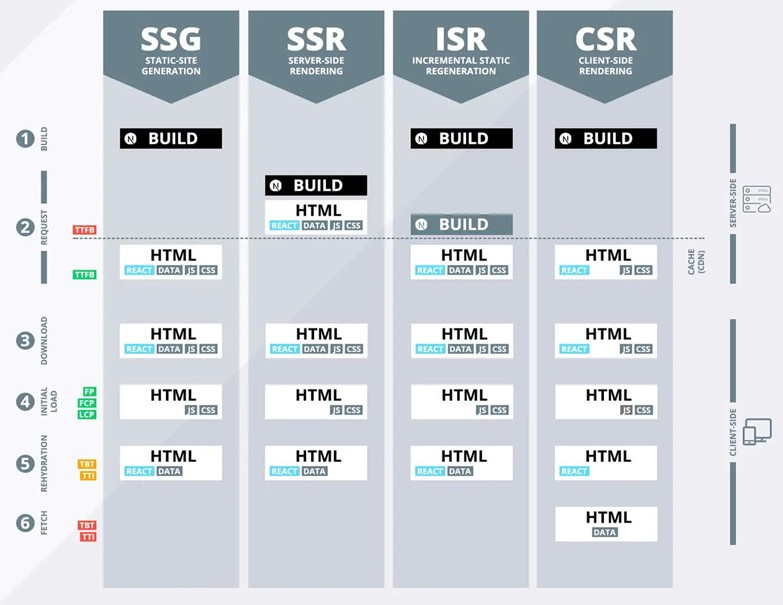
\includegraphics[width=\textwidth]{slike/pregled-strategija-iscrtavanja.jpg}
    \caption{Pregled strategija iscrtavanja u Next.js programskom okviru\cite{dumais2021nextjs}}
    \label{fig:pregled-strategija-iscrtavanja}
\end{figure}

% TODO Pregled programskih okvira ubaciti?
\newpage

\section{Metodologija}

\subsection{Opis referentne aplikacije}

Za potrebe testiranja performansi različitih programskih okvira kroz različite strategije iscrtavanja bilo je potrebno napraviti demo aplikaciju koja bi bila reprezentativna, ali ne presložena, te bi uključivala stranice sa statičnim i dinamičnim sadržajem.

\bigskip

Predstavnik statične stranice je stranica „O nama“. Ovakve stranice najčešće koriste statičan sadržaj koji se vrlo rijetko mijenja, te često čine dio web aplikacija raznih tvrtki. Dinamični dio predstavljaju stranice bloga, također popularnog sadržaja na webu.

\bigskip

Kako bi se održala konzistentnost implementacije u svim programskim okvirima navedene stranice imaju istu strukturu (HTML) i za stiliziranje koriste Tailwind CSS okvir koji je vrlo popularan i raširen zbog svoje jednostavnosti korištenja i integracije sa modernim programskim okvirima.

\bigskip

Za font je korišten Google font obitelji Archivo. Sve slike osim open graph sike poslužuju se kroz servis Lorem Picsum prema id-ju ili seedu kako bi se izbjeglo učitavanje nasumičnih slika pri svakoj posjeti stranice. Za dohvaćanje sadržaja bloga korišten je popularni servis za posluživanje testnih podataka JSONPlaceholder.

\bigskip

\begin{figure}[H]
    \centering
    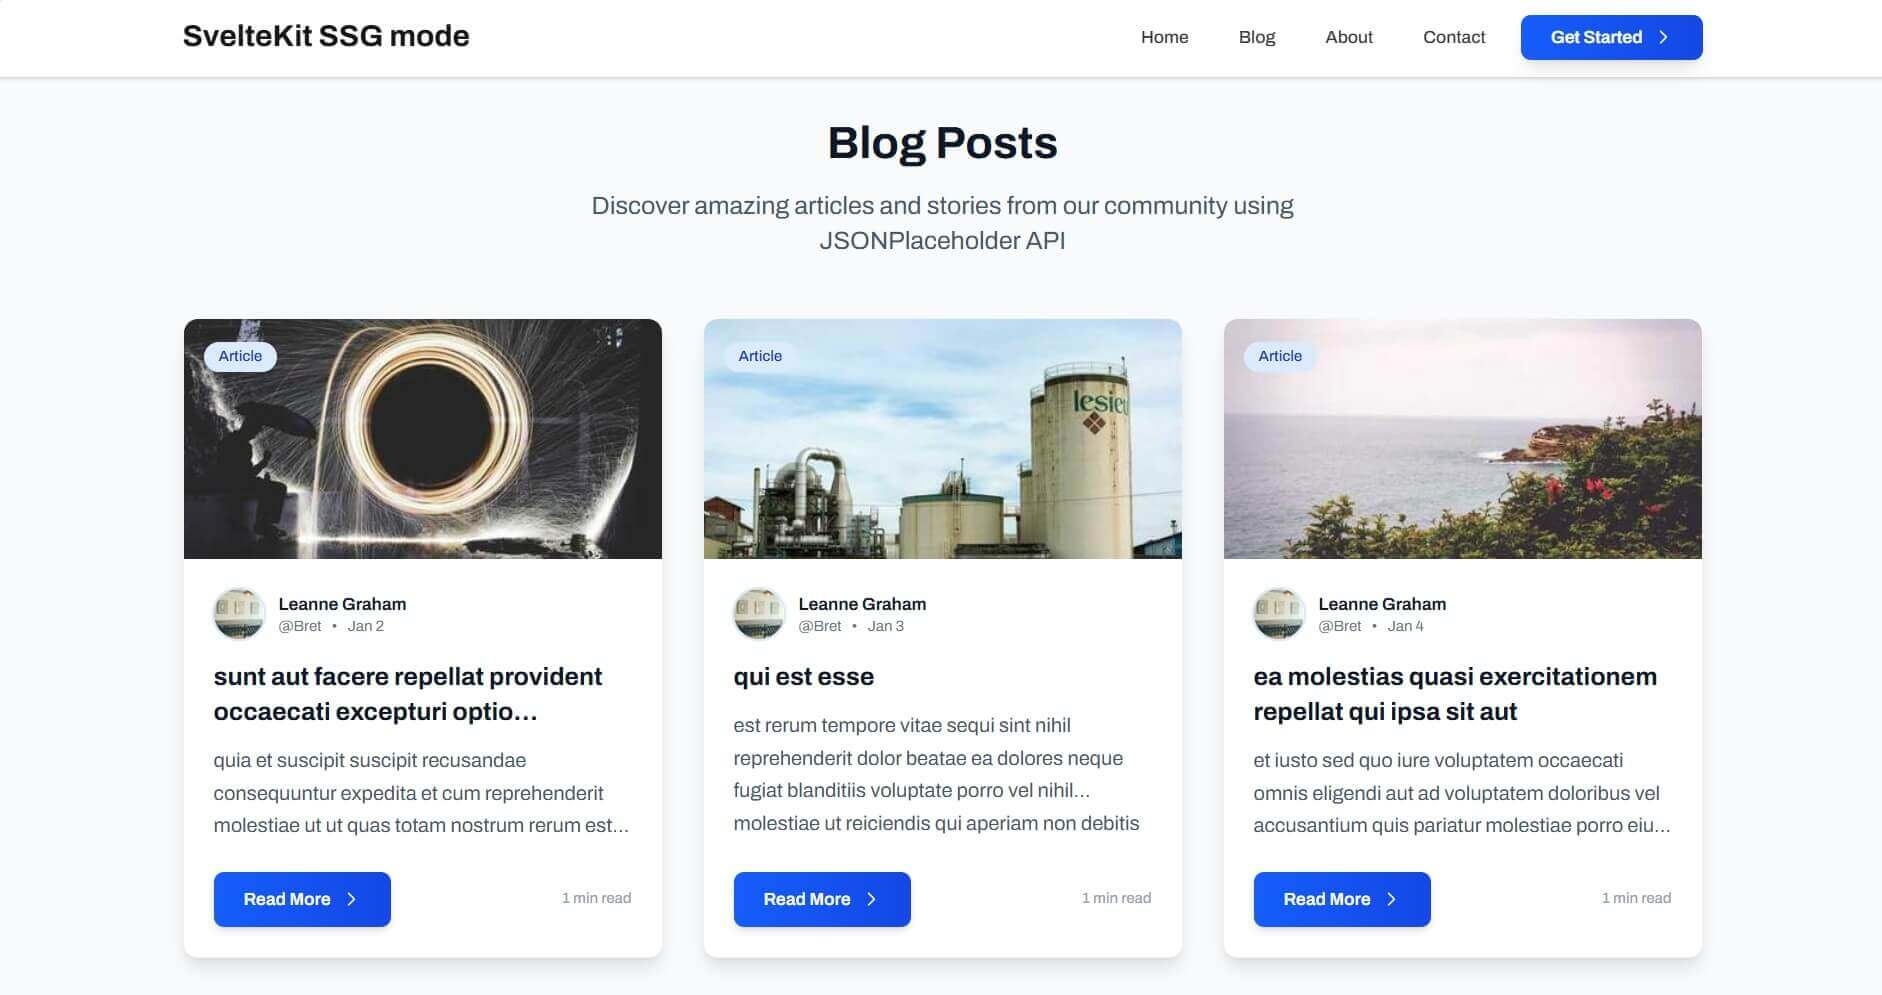
\includegraphics[width=\textwidth]{slike/metodologija/prikaz-blog-stranice.jpg}
    \caption{Prikaz blog podstranice}
    \label{fig:prikaz-blog-stranice}
\end{figure}

\subsection{Implementacija u programskim okvirima}
Work in progress
% TODO ovo poglavlje napisati

\subsection{Mjerene metrike Performansi}

Za mjerenje performansi aplikacije odabrane su standardne metrike poznate pod nazivom Web vitals nastale na Googleovu inicijativu kako bi se standardiziralo mjerenje performansi i dobio bolji uvid u korisničko iskustvo. Osim glavnih metrika u istraživanje su uključene i dodatne metrike poput vremena izgradnje, vremena skriptiranja i veličine JavaScript paketa koji se dostavlja klijentu. Slijedi kratak pregled svih korištenih metrika.

\subsection{Iscrtavanje najvećeg sadržaja (LCP)}

LCP, odnosno „Largest Contentful Paint“, mjeri koliko je vremena potrebno da se na stranici prikaže njen najveći vidljivi element. Proteklo vrijeme do 2,5 sekunde smatra se dobrim pokazateljem performansi. U obzir se uzima samo onaj dio elementa koji korisnik može vidjeti – dijelovi koji su odrezani ili nisu vidljivi se zanemaruju. Tijekom učitavanja stranice, koje se često odvija u nekoliko koraka, taj najveći element može se promijeniti. Prvo se zabilježi vrijeme učitavanja tada najvećeg elementa, a ako se kasnije pojavi još veći, mjeri se vrijeme učitavanja novog elementa. Kada korisnik počne koristiti stranicu, preglednik prestaje pratiti nove elemente jer interakcije mogu promijeniti ono što je vidljivo. LCP se zato koristi kao pokazatelj trenutka kada je glavni sadržaj stranice postao dostupan korisniku \cite{nordstrom2023comparison}.

\subsection{Ukupno vrijeme blokiranja (TBT)}

TBT (engl. Total Blocking Time) predstavlja ukupan vremenski period koji protekne od otvaranja stranice do trenutka kada korisnik može normalno stupiti u interakciju s njom. Pod interakcijom se podrazumijevaju radnje poput klika mišem, dodira zaslona ili unosa putem tipkovnice. Vrijeme se računa tako da se zbroje svi dijelovi dugih zadataka (onih koji traju više od 50 milisekundi), a koji sprječavaju preglednik da odmah odgovori na korisničke radnje. Ovi se zadaci bilježe u razdoblju između početnog prikaza sadržaja (FCP) i trenutka kada stranica postane potpuno funkcionalna. Sve što prelazi granicu od 50 ms kod pojedinog zadatka ulazi u ukupnu vrijednost TBT-a \cite{nordstrom2023comparison}.

\subsection{Kumulativna promjena rasporeda (CLS)}

Pomicanje sadržaja na web stranici tijekom njenog učitavanja naziva se  pomak izgleda (engl. layout shift). Do toga najčešće dolazi zbog asinkronog učitavanja sadržaja ili dodavanja novih DOM elemenata preko postojećih komponenti. CLS prati najveći niz takvih pomaka koji se dogode unutar jednog vremenskog okvira od maksimalno 5 sekundi, pri čemu između pojedinih pomaka ne smije proći više od jedne sekunde. Ova metrike je važna jer pokazuje stabilnost stranice, a poželjno je da rezultat bude što niži – vrijednost 0.1 smatra se dobrim rezultatom \cite{nordstrom2023comparison}.

\subsection{Vrijeme do interaktivnosti (TTI)}

Ova metrika označava koliko je vremena potrebno da web stranica postane potpuno interaktivna. To znači da se prvo prikaže koristan sadržaj (što mjeri FCP), zatim da stranica reagira na korisničke radnje u roku kraćem od 50 milisekundi te da je većina upravljača događaja (engl. event handler) učitana i spremna. Vrijeme kraće od 3,8 sekundi smatra se dobrim rezultatom. Spor TTI često je uzrokovan loše optimiziranim JavaScript kodom. \cite{nordstrom2023comparison}

\subsection{Vrijeme do prvog bajta (TTFB)}

Vrijeme do prvog bajta označava koliko vremena prođe od trenutka kada preglednik pošalje zahtjev prema serveru do trenutka kada primi prvi bajt povratnog odgovora. Ova metrika prikazuje koliko brzo se uspostavlja veza i koliko brzo server reagira, uključujući sve faze poput preusmjeravanja, DNS rezolucije, TLS dogovora i slanja zahtjeva. Niža vrijednost TTFB-a znači da se stranica učitava brže, što pozitivno utječe i na ostale važne metrike poput FCP-a. Idealno bi bilo da TTFB ostane ispod 0,8 sekundi radi optimalnog korisničkog iskustva \cite{pollardttfb}.

\subsection{Dodatne metrike}

\begin{itemize}
    \item Veličina paketa (engl. bundle size) predstavlja ukupnu veličinu svih JavaScript datoteka koje se preuzimaju prilikom početnog učitavanja stranice – uključujući sve JS dijelove potrebne za prikaz početne stranice.
    \item Vrijeme izgradnje (engl. build time) odnosi se na trajanje procesa generiranja statičkih stranica prilikom pretvaranja izvornog koda u izvršni kod. Vrijeme izgradnje može se očitati iz terminala prilikom lokalne izgradnje ili pak iz Vercelovih zapisa izgradnje (eng. build logs).
    \item Ukupno trajanje izvršavanja skripti (engl. total scripting time) predstavlja zbroj vremena izvršavanja svih JavaScript skripti na stranici. Ova metrika pomaže pri identifikaciji potencijalnih uskih grla u performansama aplikacije.
\end{itemize}


\subsection{Lighthouse}

Glavni i de facto standard za testiranje performansi web aplikacija je Googleov alat otvorenog koda imena Lighthouse. Ovaj alat integriran je u Chrome preglednik, ali i dostupan kao zasebna CLI aplikacija. Pruža sve što je potrebno za provođenje testova performansi i SEO-a i generiranje izvještaja u različitim formatima, što ga čini vrlo funkcionalnim i korisnim u unapređivanju tehničke strane web aplikacija i korisničkog iskustva \cite{googlelighthouse}.

\subsection{Chrome DevTools}

Chrome DevTools je set alata unutar Chrome preglednika koji između ostalog omogućuju analizu performansi web stranice. U kontekstu ovog rada najvažniji su paneli Performance i Network koji prikazuju brzinu učitavanja stranice i resursa. Ključna funkcionalnost je Performance Insights, koja snima korisničku sesiju i bilježi metrike poput FCP i LCP. Ovaj alat korišten je u analizi veličine JavaScript paketa koje klijent preuzima i izvršava \cite{nordstrom2023comparison}.

\subsection{Lighthouse reporter}

Za potrebe ovog rada bilo je potrebno izvesti 360 Lighthouse testova\footnote{3 aplikacije * 4 strategije iscrtavanja * 10 testova po kombinaciji * 3 podstranice (about, blog, blog detalji)} te prikupljene podatke obraditi, grupirati i sažeti (izraditi master tablice sa prosječnim vrijednostima). Zbog opsežnosti testiranja jedini praktični način bilo je napraviti Node.js skriptu koja će na temelju definiranih parametara koristeći Lighthouse CLI alat izvršiti sve testove i generirati datoteke s rezultatima u CSV formatu za daljnju analizu podataka.
Aplikacija za testiranje sastoji se od 3 ključna dijela:
\begin{enumerate}
    \item konfiguracijske JSON datoteke u kojoj su definirani svi parametri testiranja
    \item datoteke LightHouseTestRunner.js koja izvozi istoimenu klasu sa svim metodama važnim za različite načine testiranja
    \item datoteke cli.js koja upravlja testovima i pokreće ih kroz terminal sa odgovarajućim argumentima
\end{enumerate}

Aplikacija za testiranje stavlja korisniku na raspolaganje raznovrstan set testova (prema programskom okviru, prema strategiji iscrtavanja itd.), no za potrebe ovoga rada korištena je naredba koja pokreće testiranje svih aplikacija po određenoj podstranici.

\bigskip

Primjer naredbe u bash terminalu:
\texttt{node cli.js all slow4g blog}

Ova naredba pokreće cli.js skriptu koja testira blog podstranicu u svim aplikacijama u konfiguraciji slow4g.

\bigskip
Skripta će ovom naredbom kreirati sljedeće datoteke za podstranicu blog:
\begin{itemize}
    \item 12 datoteka sa podacima svih 10 mjerenja po programskom okviru i strategiji iscrtavanja
    \item 4 datoteke prosječnih vrijednosti za svaku strategiju iscrtavanja
    \item 1 datoteku sa ukupnim rezultatima za odabranu podstranicu (konačne prosječne vrijednosti svih 12 kombinacija)
\end{itemize}
Ova naredba ponovljena je za svaku podstranicu čime je generirana 51 datoteka\footnote{3 podstranice * 3 programska okvira * 4 strategije iscrtavanja + 12 sažetaka + 3 glavna sažetka}.
Za daljnju analizu korištene su 3 datoteke glavnih sažetaka za svaku stranicu. Svaka od tih datoteka sadrži prosječne vrijednosti testova za svaku od 12 kombinacija strategija i programskih okvira.

\bigskip

Zbog velikog broja provedenih testova, bilo je nužno osigurati njihovu potpunu uspješnost i cjelovitost podataka. Za tu svrhu u skriptu je ugrađen i mehanizam provjere uspješnosti testiranja, koji će u slučaju neuspješnog testa pokušati ponoviti test još dva puta, te ako ni tada ne uspije, naznačiti će gdje je došlo do greške i pokušati nastaviti s testiranjem. Po završetku izvršavanja test skripte moguće je ponovno inicirati izvođenje neuspješnih testova.

\bigskip

Prilikom testiranja skripte ovim mehanizmom otkrivene su greške u dvije web-aplikacije, koje su uzrokovale nedostatak određenih metrika. Zbog neispravne konfiguracije, pojedine podstranice su u produkcijskoj okolini vraćale grešku 404, što je rezultiralo nepotpunim rezultatima testiranja. Nakon ispravka konfiguracije, svi testovi su uspješno provedeni već pri prvom pokretanju.

\bigskip

Izvorni kod skripte, zajedno sa dobivenim rezultatima dostupan je na autorovom Git repozitoriju.\footnote{\url{https://github.com/AlphaActual/lighthouse-reporter}}

\begin{figure}[H]
    \centering
    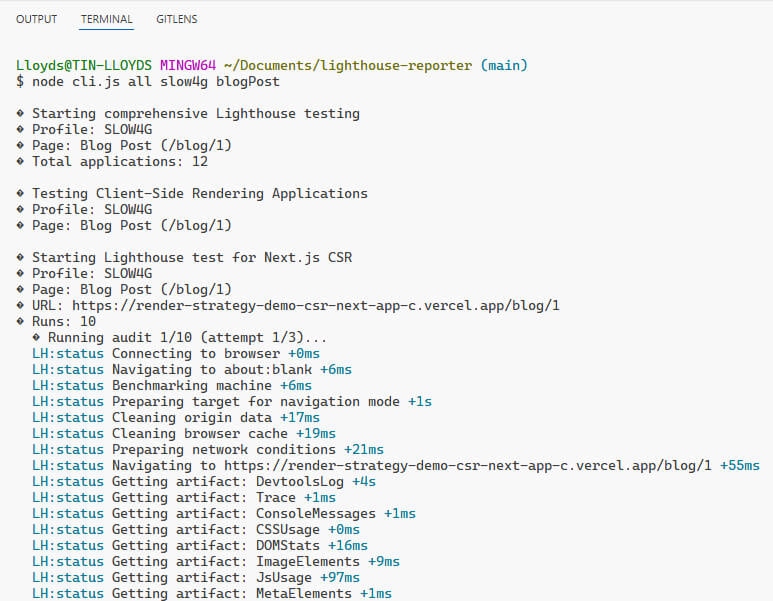
\includegraphics[width=\textwidth]{slike/metodologija/testiranje-aplikacije.jpg}
    \caption{Testiranje stranice pojedinog bloga kroz terminal}
    \label{fig:testiranje-aplikacije}
\end{figure}

\subsection{Struktura i prikaz podataka}

Prikupljeni podaci svake metrike dobivene CLI alatom Lighthouse pretvoreni su u mjerne jedinice prigodne za daljnju analizu i bolju interpretaciju rezultata. Npr. milisekunde su najprije pretvorene u sekunde, vrijednosti CLS (raspon od 0 do 1) su normalizirane i zaokružene na 3 decimale tako da se lakše uspoređuju između različitih testova. Uz izvorne vrijednosti u CSV datoteke s rezultatima pohranjene su i vrijednosti ocjene koju je tom rezultatu dodijelio Lighthouse.

\bigskip

Lighthouse svaki sirovi podatak pretvara u ocjenu od 0 do 100, gdje je 100 najbolja ocjena. Ovu ocjenu Lighthouse dodjeljuje na temelju krivulje distribucije izvedene iz stvarnih podataka o performansama web-stranica prikupljenih na HTTP Archiveu \cite
{chrome2025lighthouse}.

\bigskip

Budući da se prikaz rezulatata oslanja na ovu ocjenu Googleovog alata koja se prigodno izražava kao postotak, na većini grafova u ovom radu prikazane su ocjene učinka i postignuti rezulatati u obliku postotka. Uz određene rezultate prikazana je i standardna devijacija.

\subsection{Testno okruženje}

Kako bi se osigurali konzistentni uvjeti testiranja koji odgovaraju stvarnom korisničkom iskustvu, te omogućila podrška za specifične strategije iscrtavanja (kao što je ISR), odabran je sljedeći pristup.

\bigskip

Sve aplikacije postavljene su na platformu Vercel koja u trenutku pisanja ovog rada jedina podržava sve odabrane strategije iscrtavanja za svaki od prethodno navedenih programskih okvira. Ovo osigurava maksimalnu kompatibilnost i integraciju bez kompliciranih konfiguracija \cite{vercelframeworks}.

\bigskip

Vercel platforma također omogućava globalnu distribuciju putem CDN-a, što znači da se sadržaji serviraju iz čvorova najbližih korisniku. Zbog ovoga i činjenice da su sve aplikacije i njihov izvorni kod javno dostupni na Internetu, moguće je provođenje dodatnih istraživanja i proširivanja ovog rada, te osiguravanje relevantnosti podataka, bez obzira na geografsku lokaciju računala na kojem bi se potencijalno radila nova testiranja.
Testiranja provedena u ovom radu izvršena su na slijedećoj računalnoj konfiguraciji:

\bigskip

\begin{itemize}
    \item Model: Lenovo IdeaPad Slim 5 16ABR8
    \item Procesor: AMD Ryzen 5 7530U sa Radeon grafikom - 2.00 GHz
    \item Radna memorija: 16.0 GB (13.9 GB iskoristivo)
    \item Tip sustava: 64-bitni operacijski sustav, procesor baziran na arhitekturi x64
    \item Verzija operacijskog sustava: Windows 11 Home (24H2)
    \item Instalirana Node.js verzija: v22.14.0
\end{itemize}

Prije izvođenja testiranja zabilježeni su slijedeći mrežni uvjeti korištenjem Speedtest web alata:

\begin{itemize}
    \item Server: Tehnoline Telekom 45.142.9.180
    \item Ping: 15ms
    \item Jitter: 2ms
    \item Download: 291.6 Mbps
    \item Upload: 102.0 Mbps
\end{itemize}

\newpage

\section{Rezultati}

\subsection{Stranica O nama}

\begin{figure}[H]
    \centering
    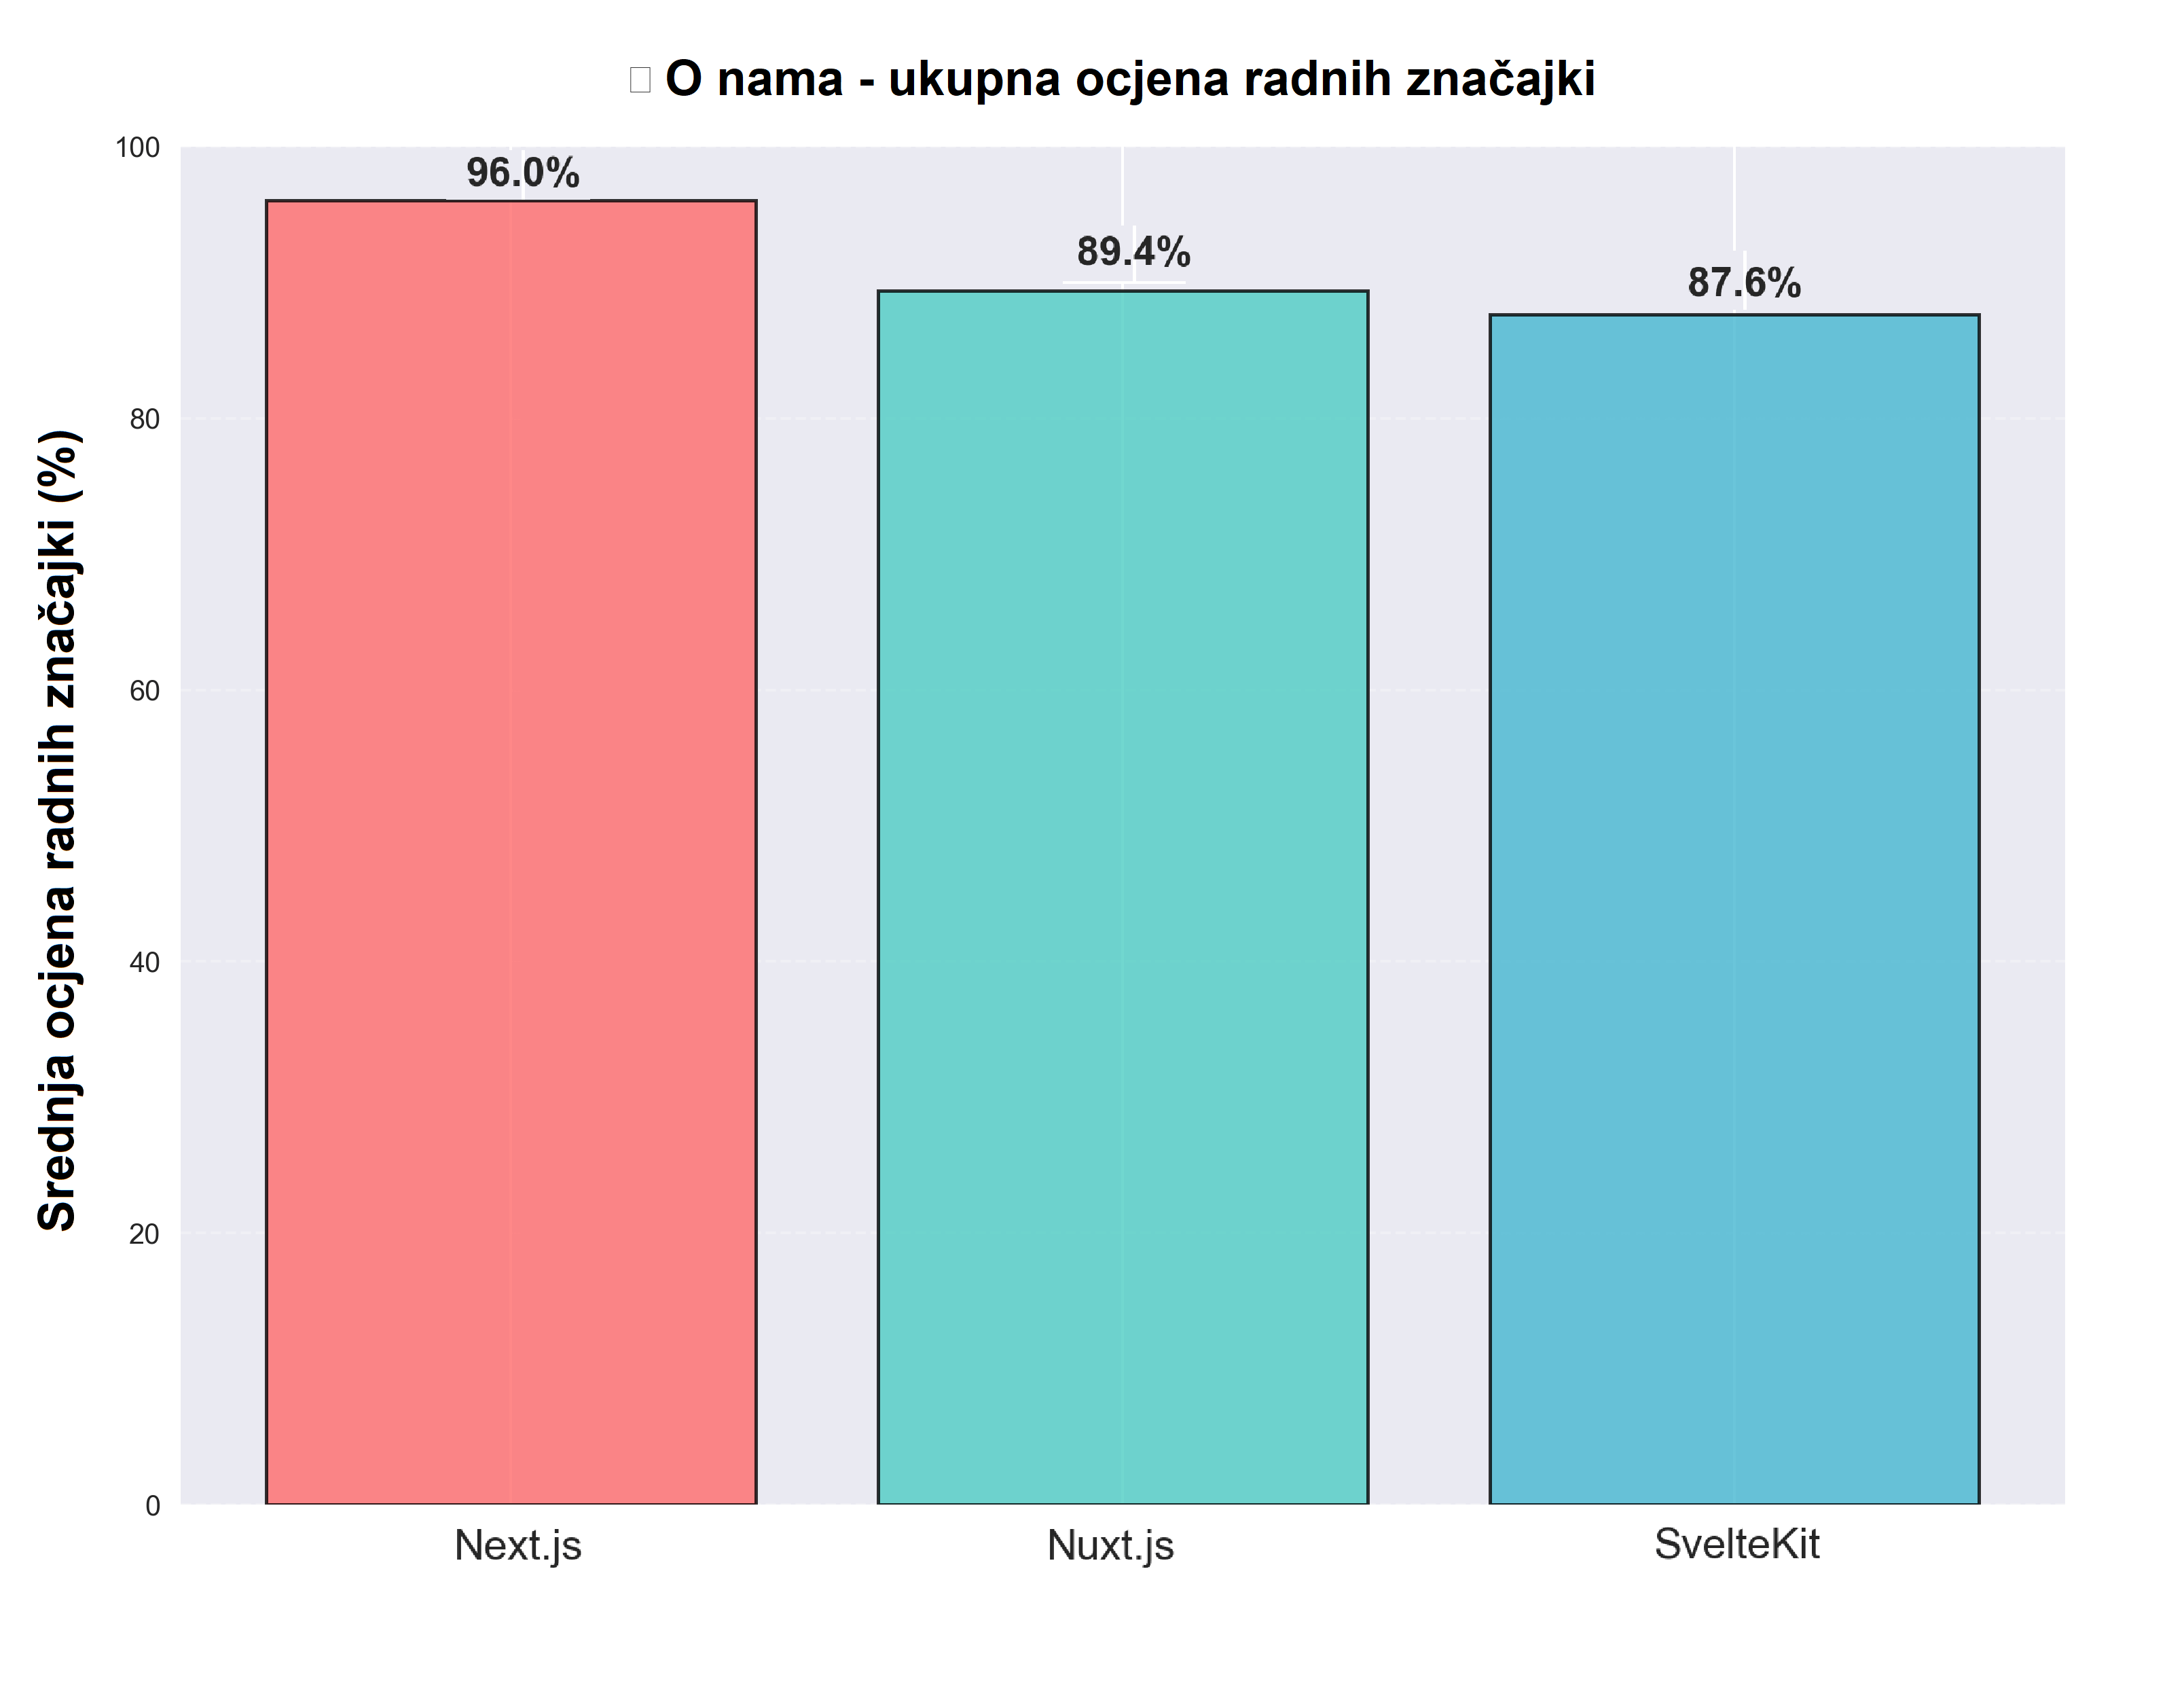
\includegraphics[width=0.8\textwidth]{slike/rezultati/about/about_framework_overall_performance.png}
    \caption{Ukupne performanse programskih okvira (stranica O nama)}
    \label{fig:testiranje-o-nama-ukupne-performanse}
\end{figure}

\begin{figure}[H]
    \centering
    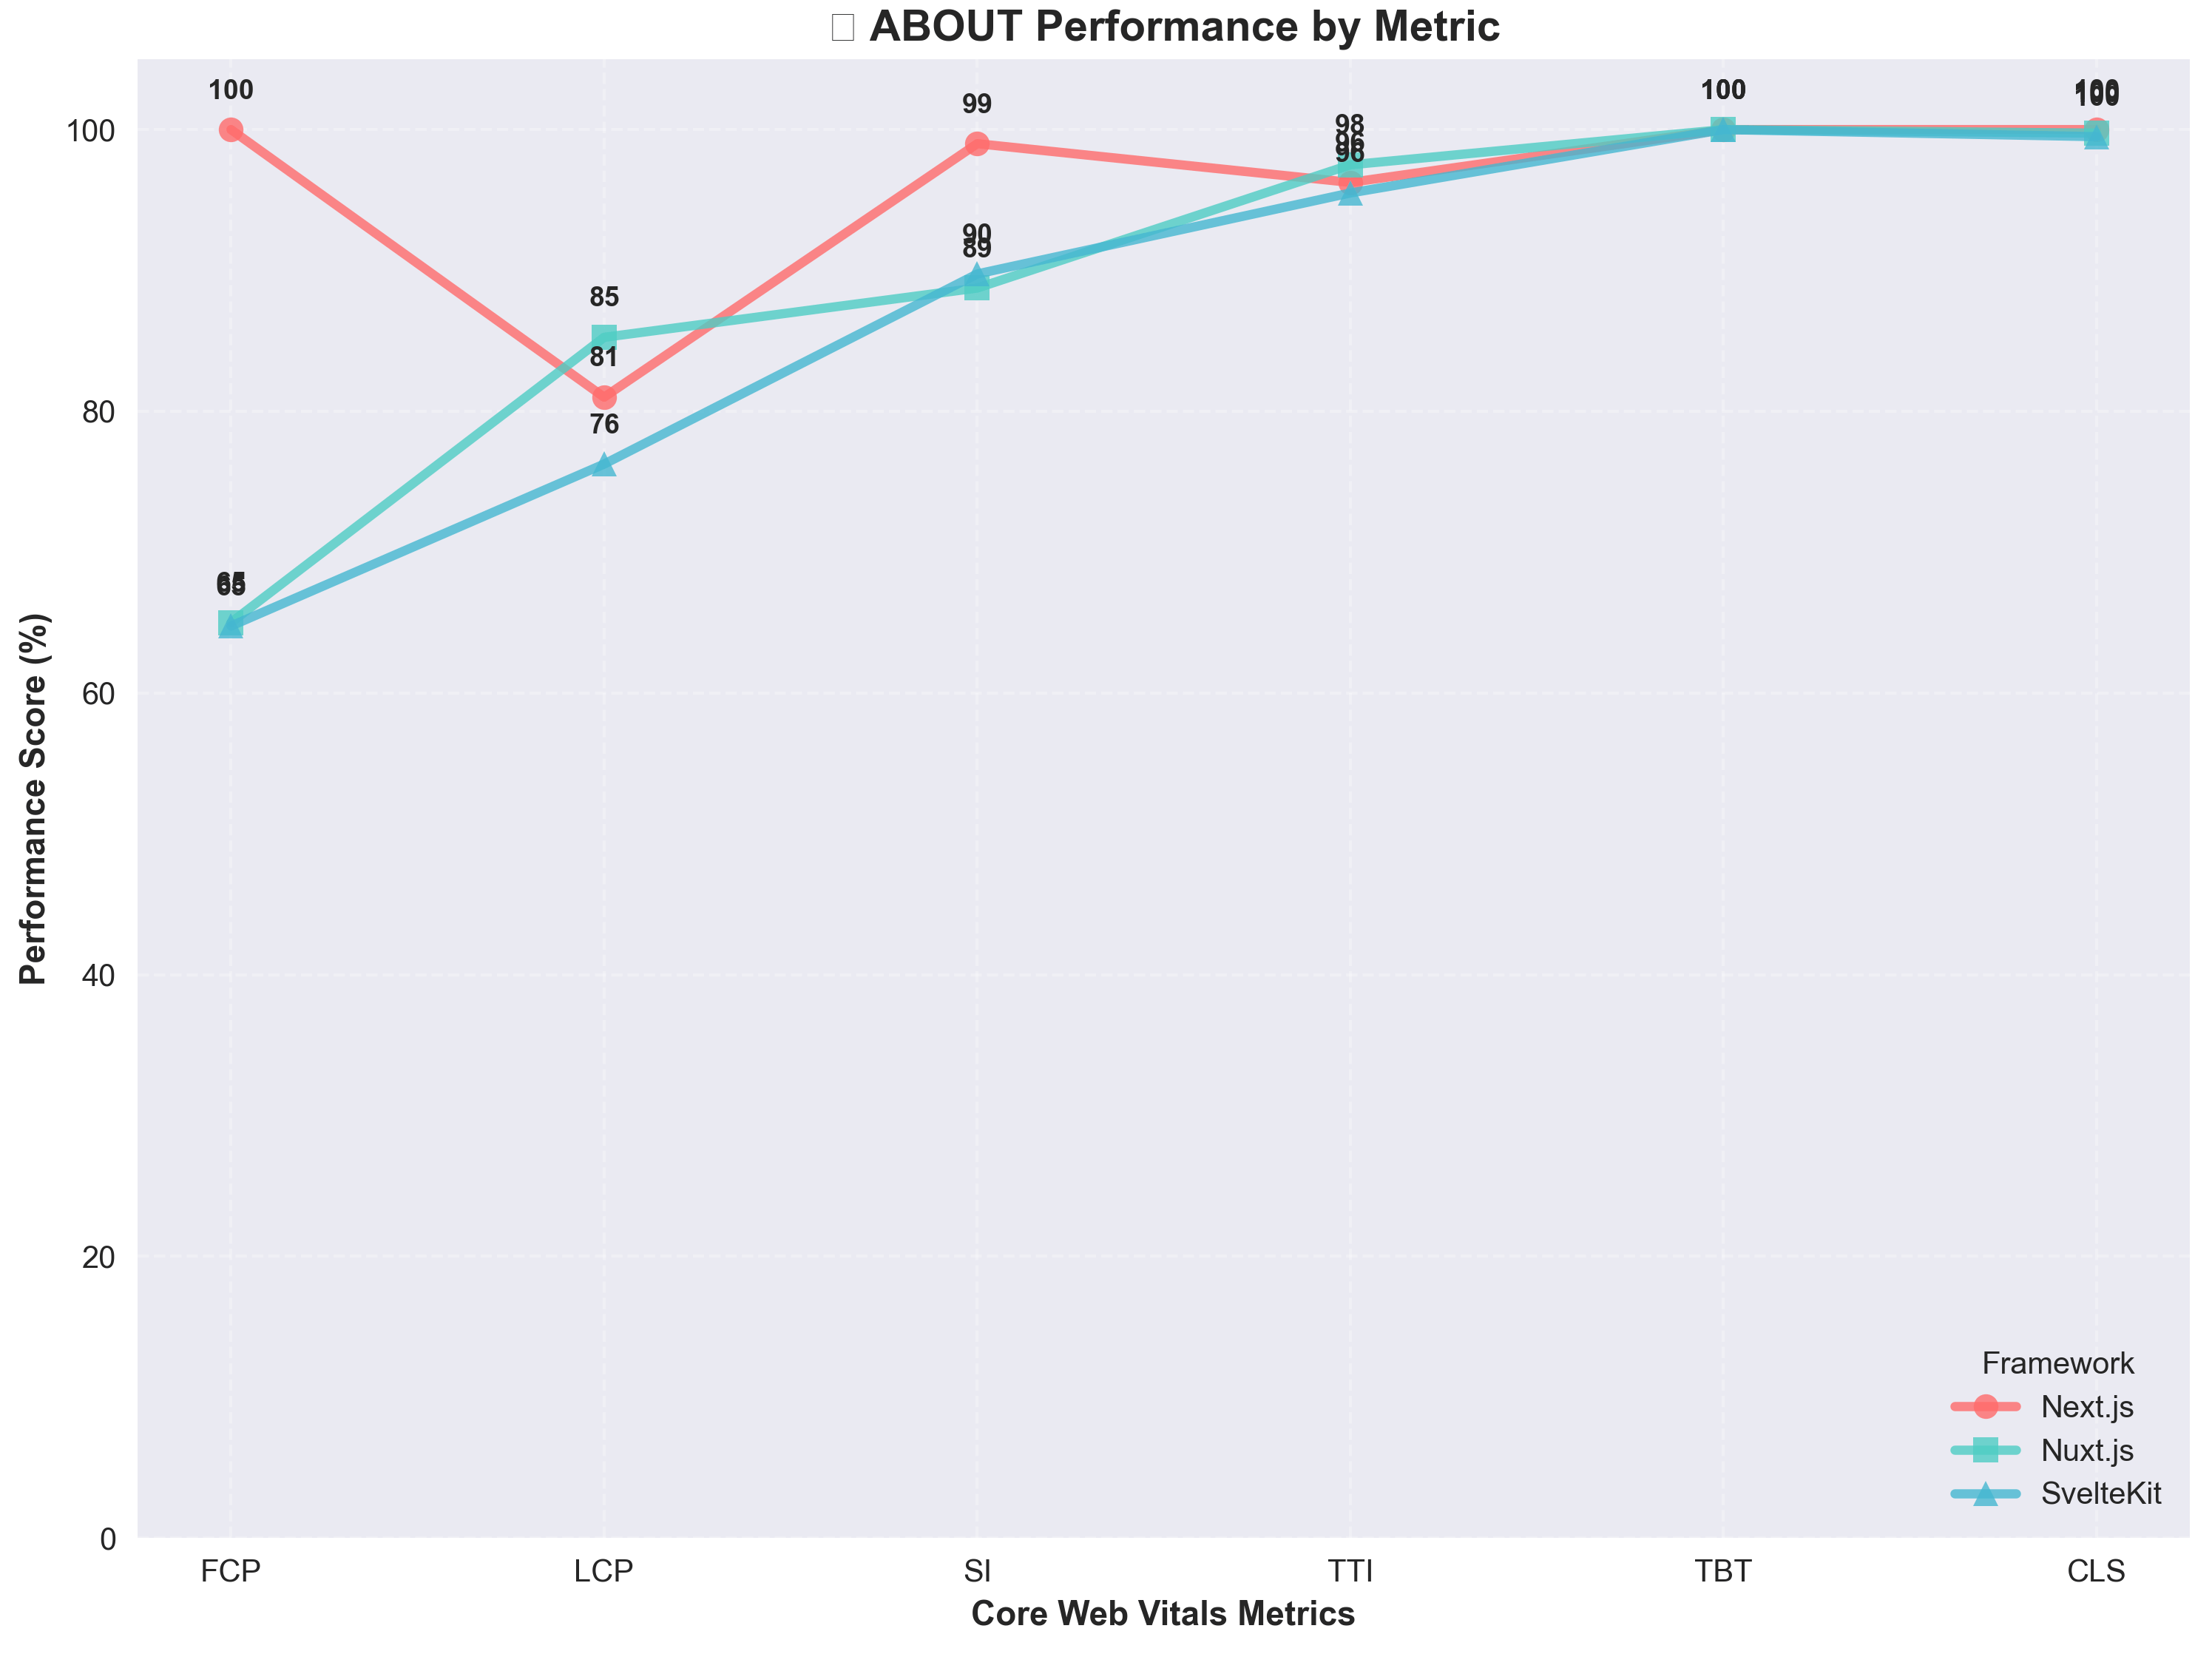
\includegraphics[width=0.8\textwidth]{slike/rezultati/about/about_performance_by_metric.png}
    \caption{Ukupne performanse programskih okvira po metrici (stranica O nama)}
    \label{fig:testiranje-o-nama-performanse-po-metrici}
\end{figure}

\begin{figure}[H]
    \centering
    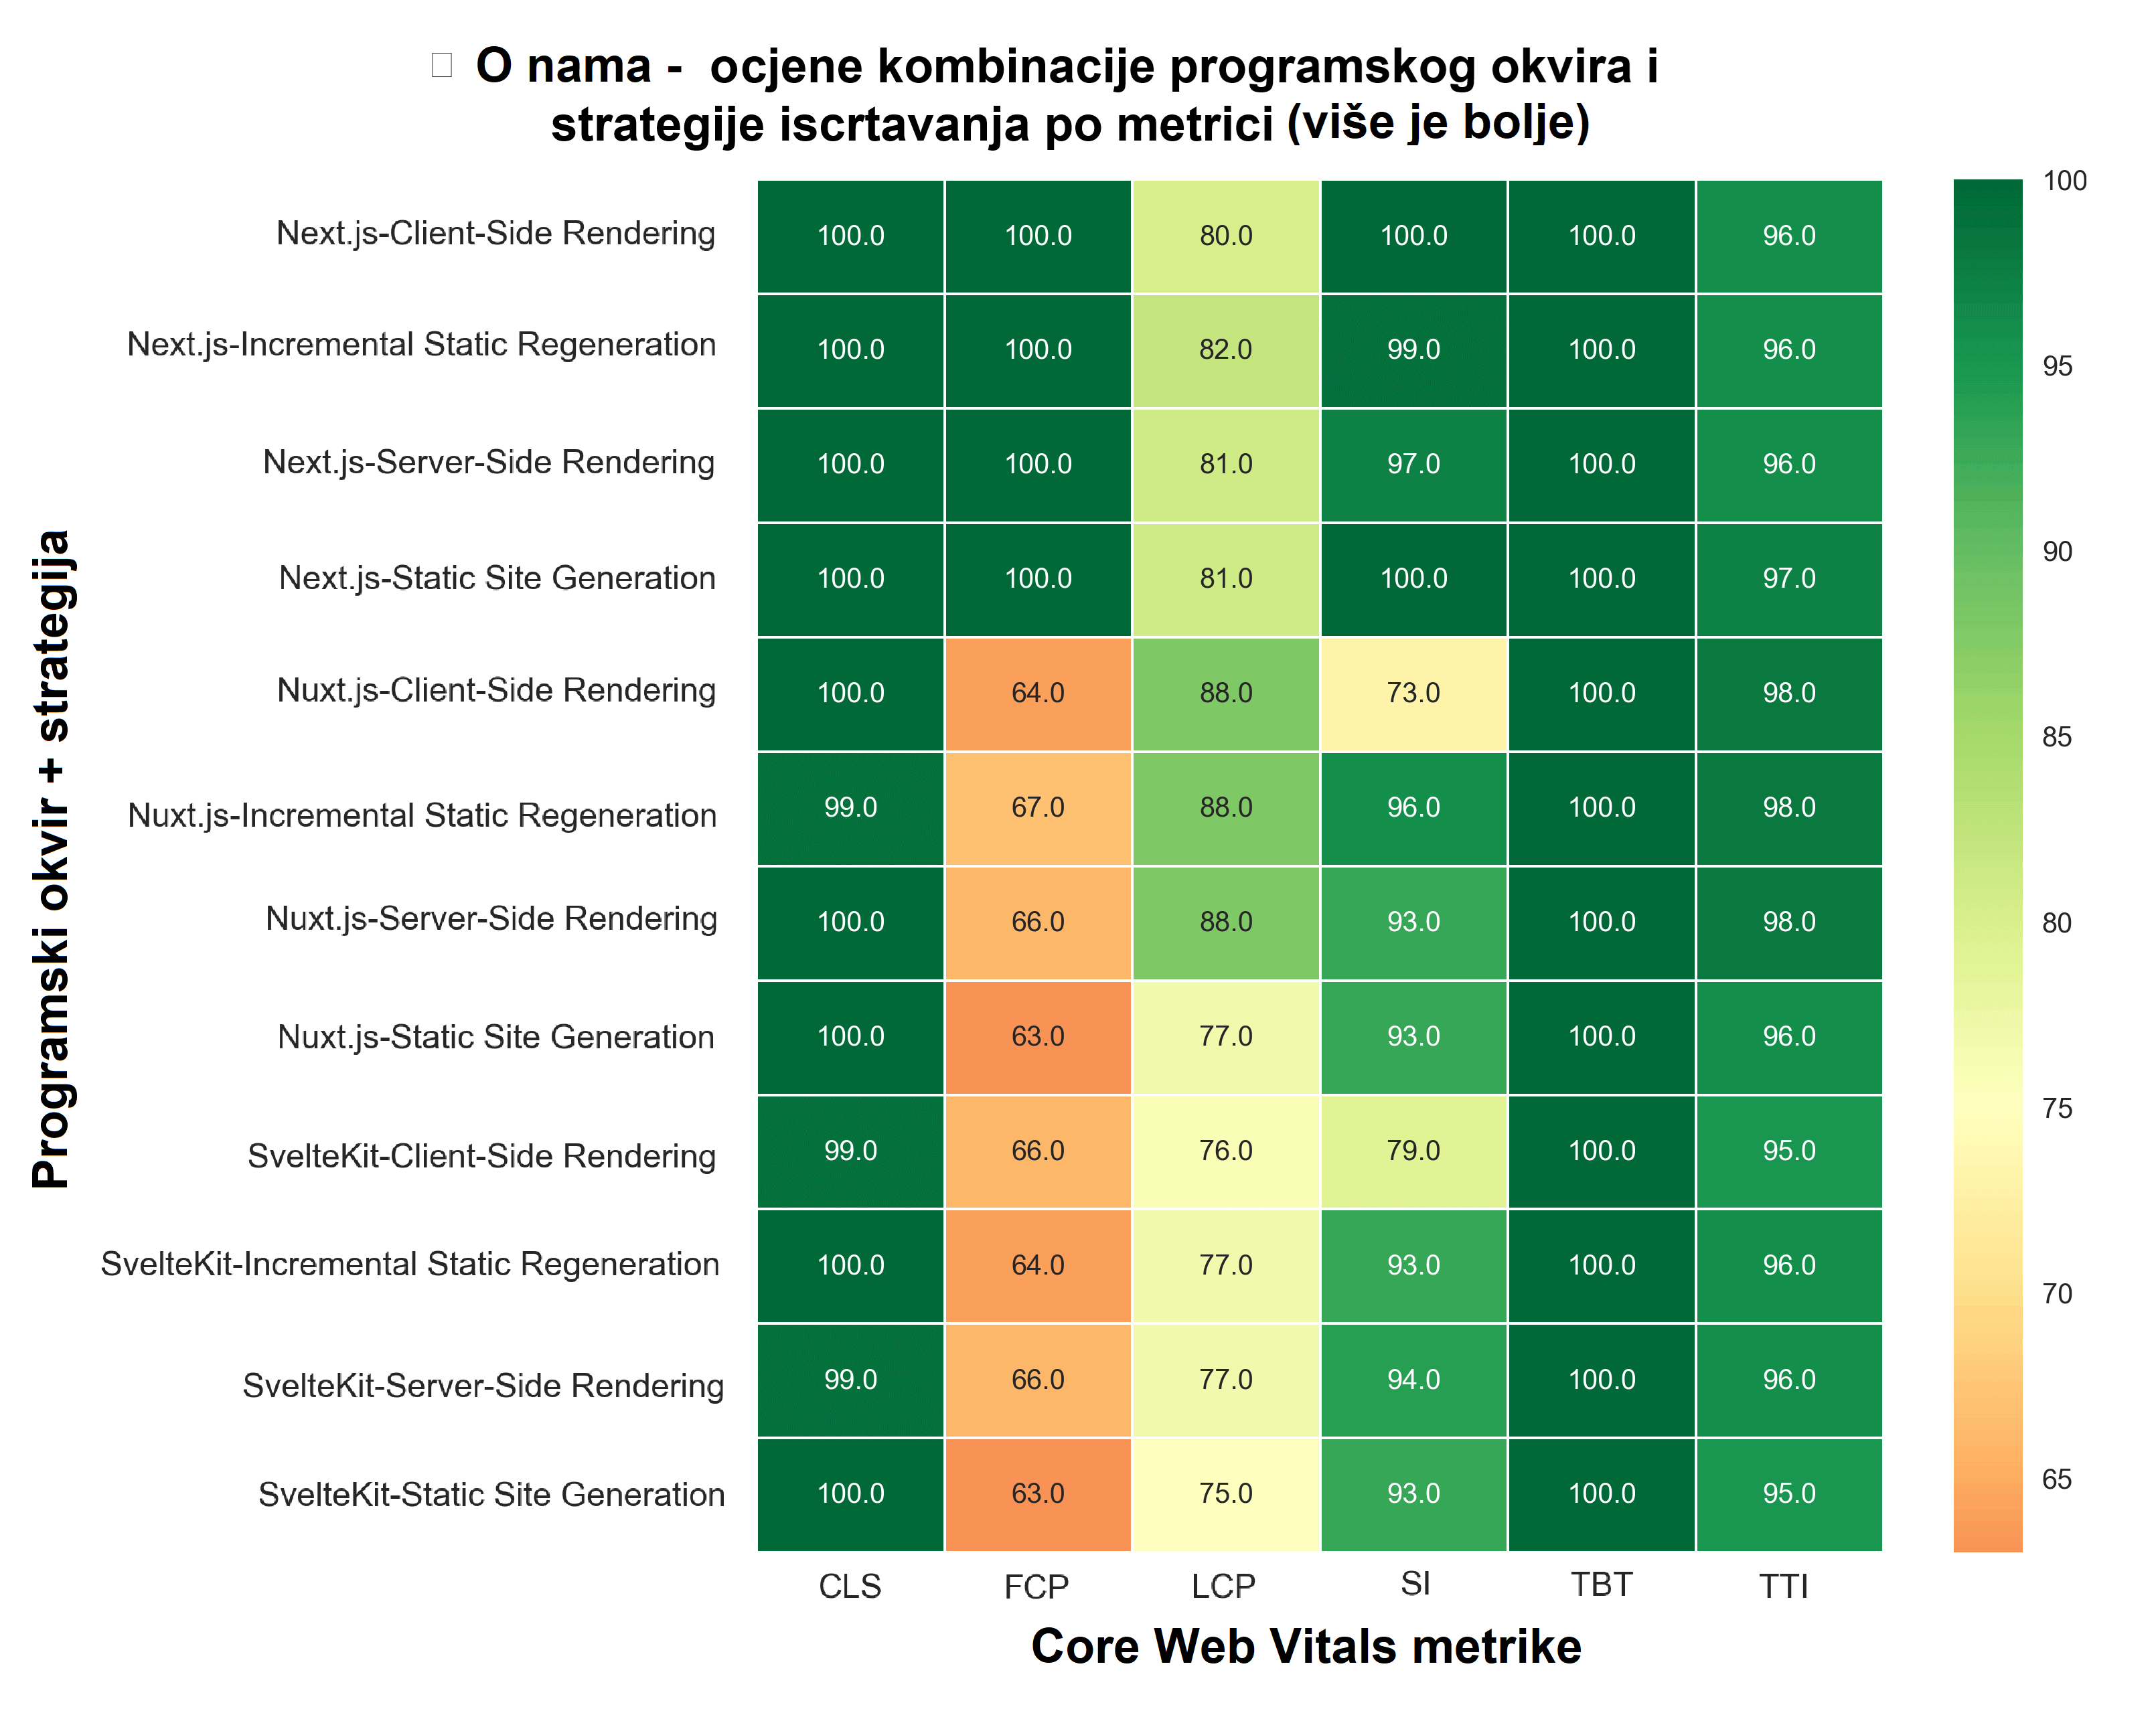
\includegraphics[width=\textwidth]{slike/rezultati/about/about_performance_scores.png}
    \caption{Performanse programskih okvira - postotak (stranica O nama)}
    \label{fig:testiranje-o-nama-postotak}
\end{figure}

\begin{figure}[H]
    \centering
    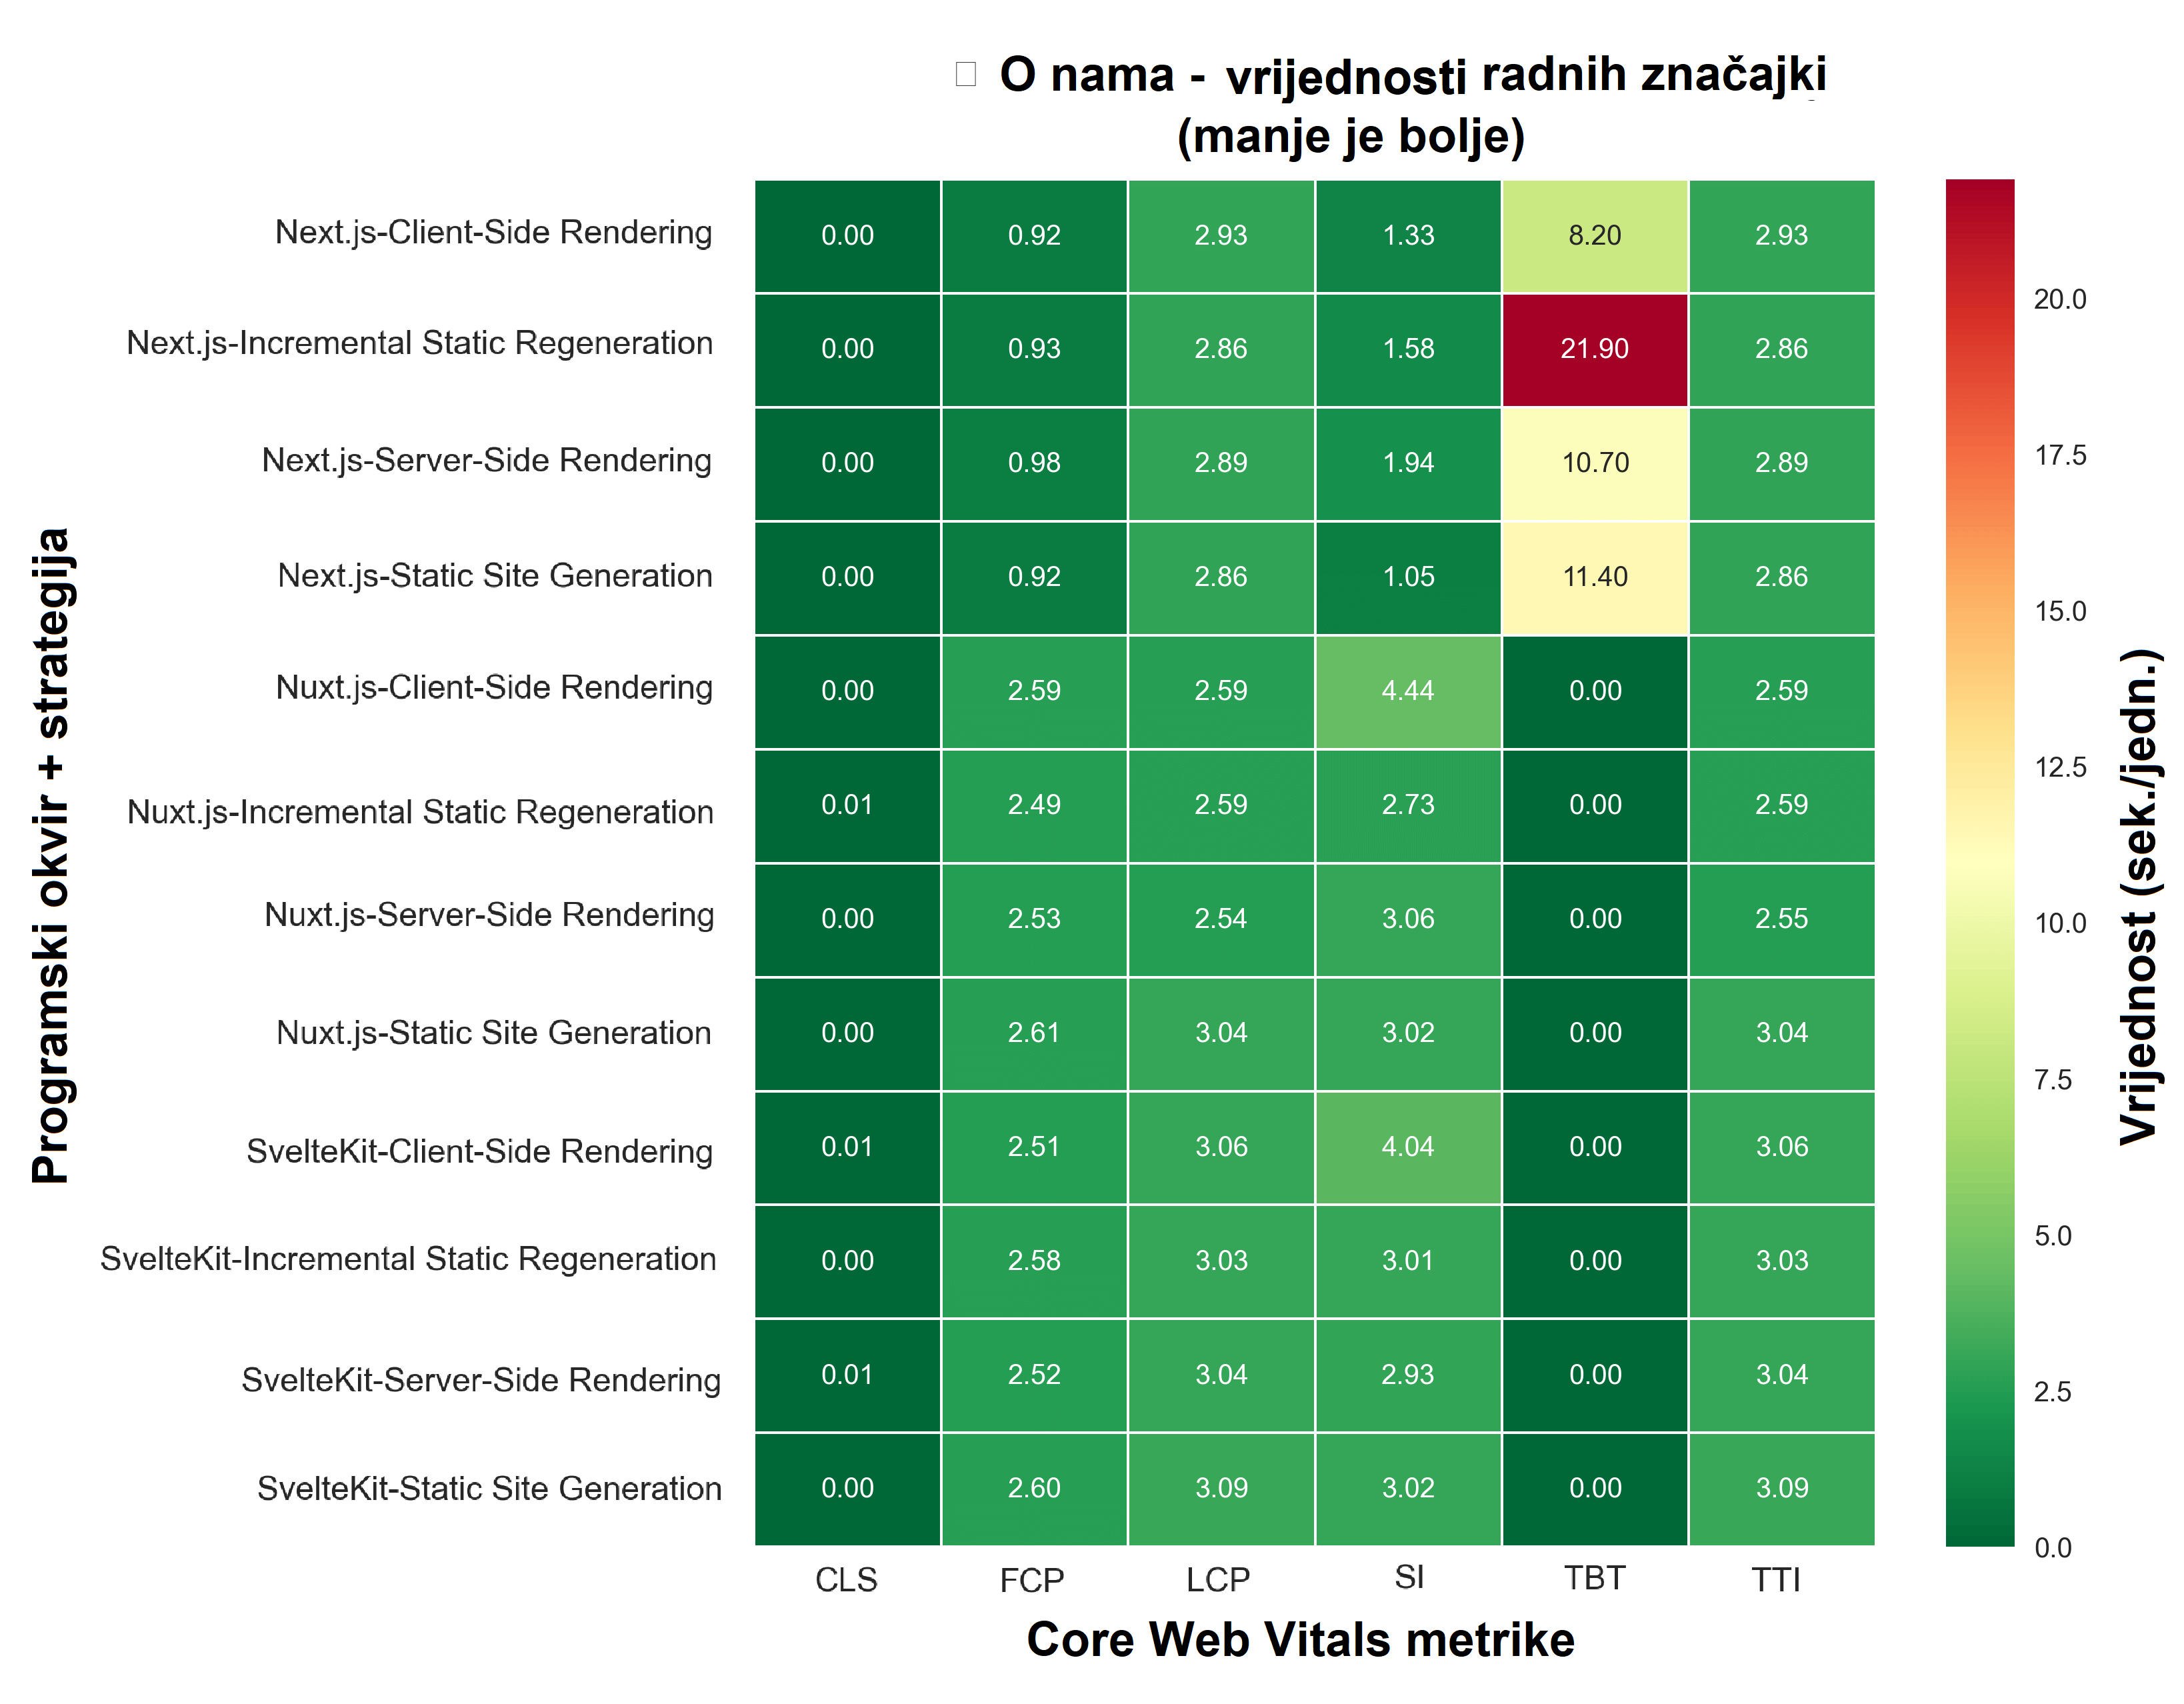
\includegraphics[width=\textwidth]{slike/rezultati/about/about_performance_values.png}
    \caption{Performanse programskih okvira - vrijednosti (stranica O nama)}
    \label{fig:testiranje-o-nama-vrijednosti}
\end{figure}

\begin{figure}[H]
    \centering
    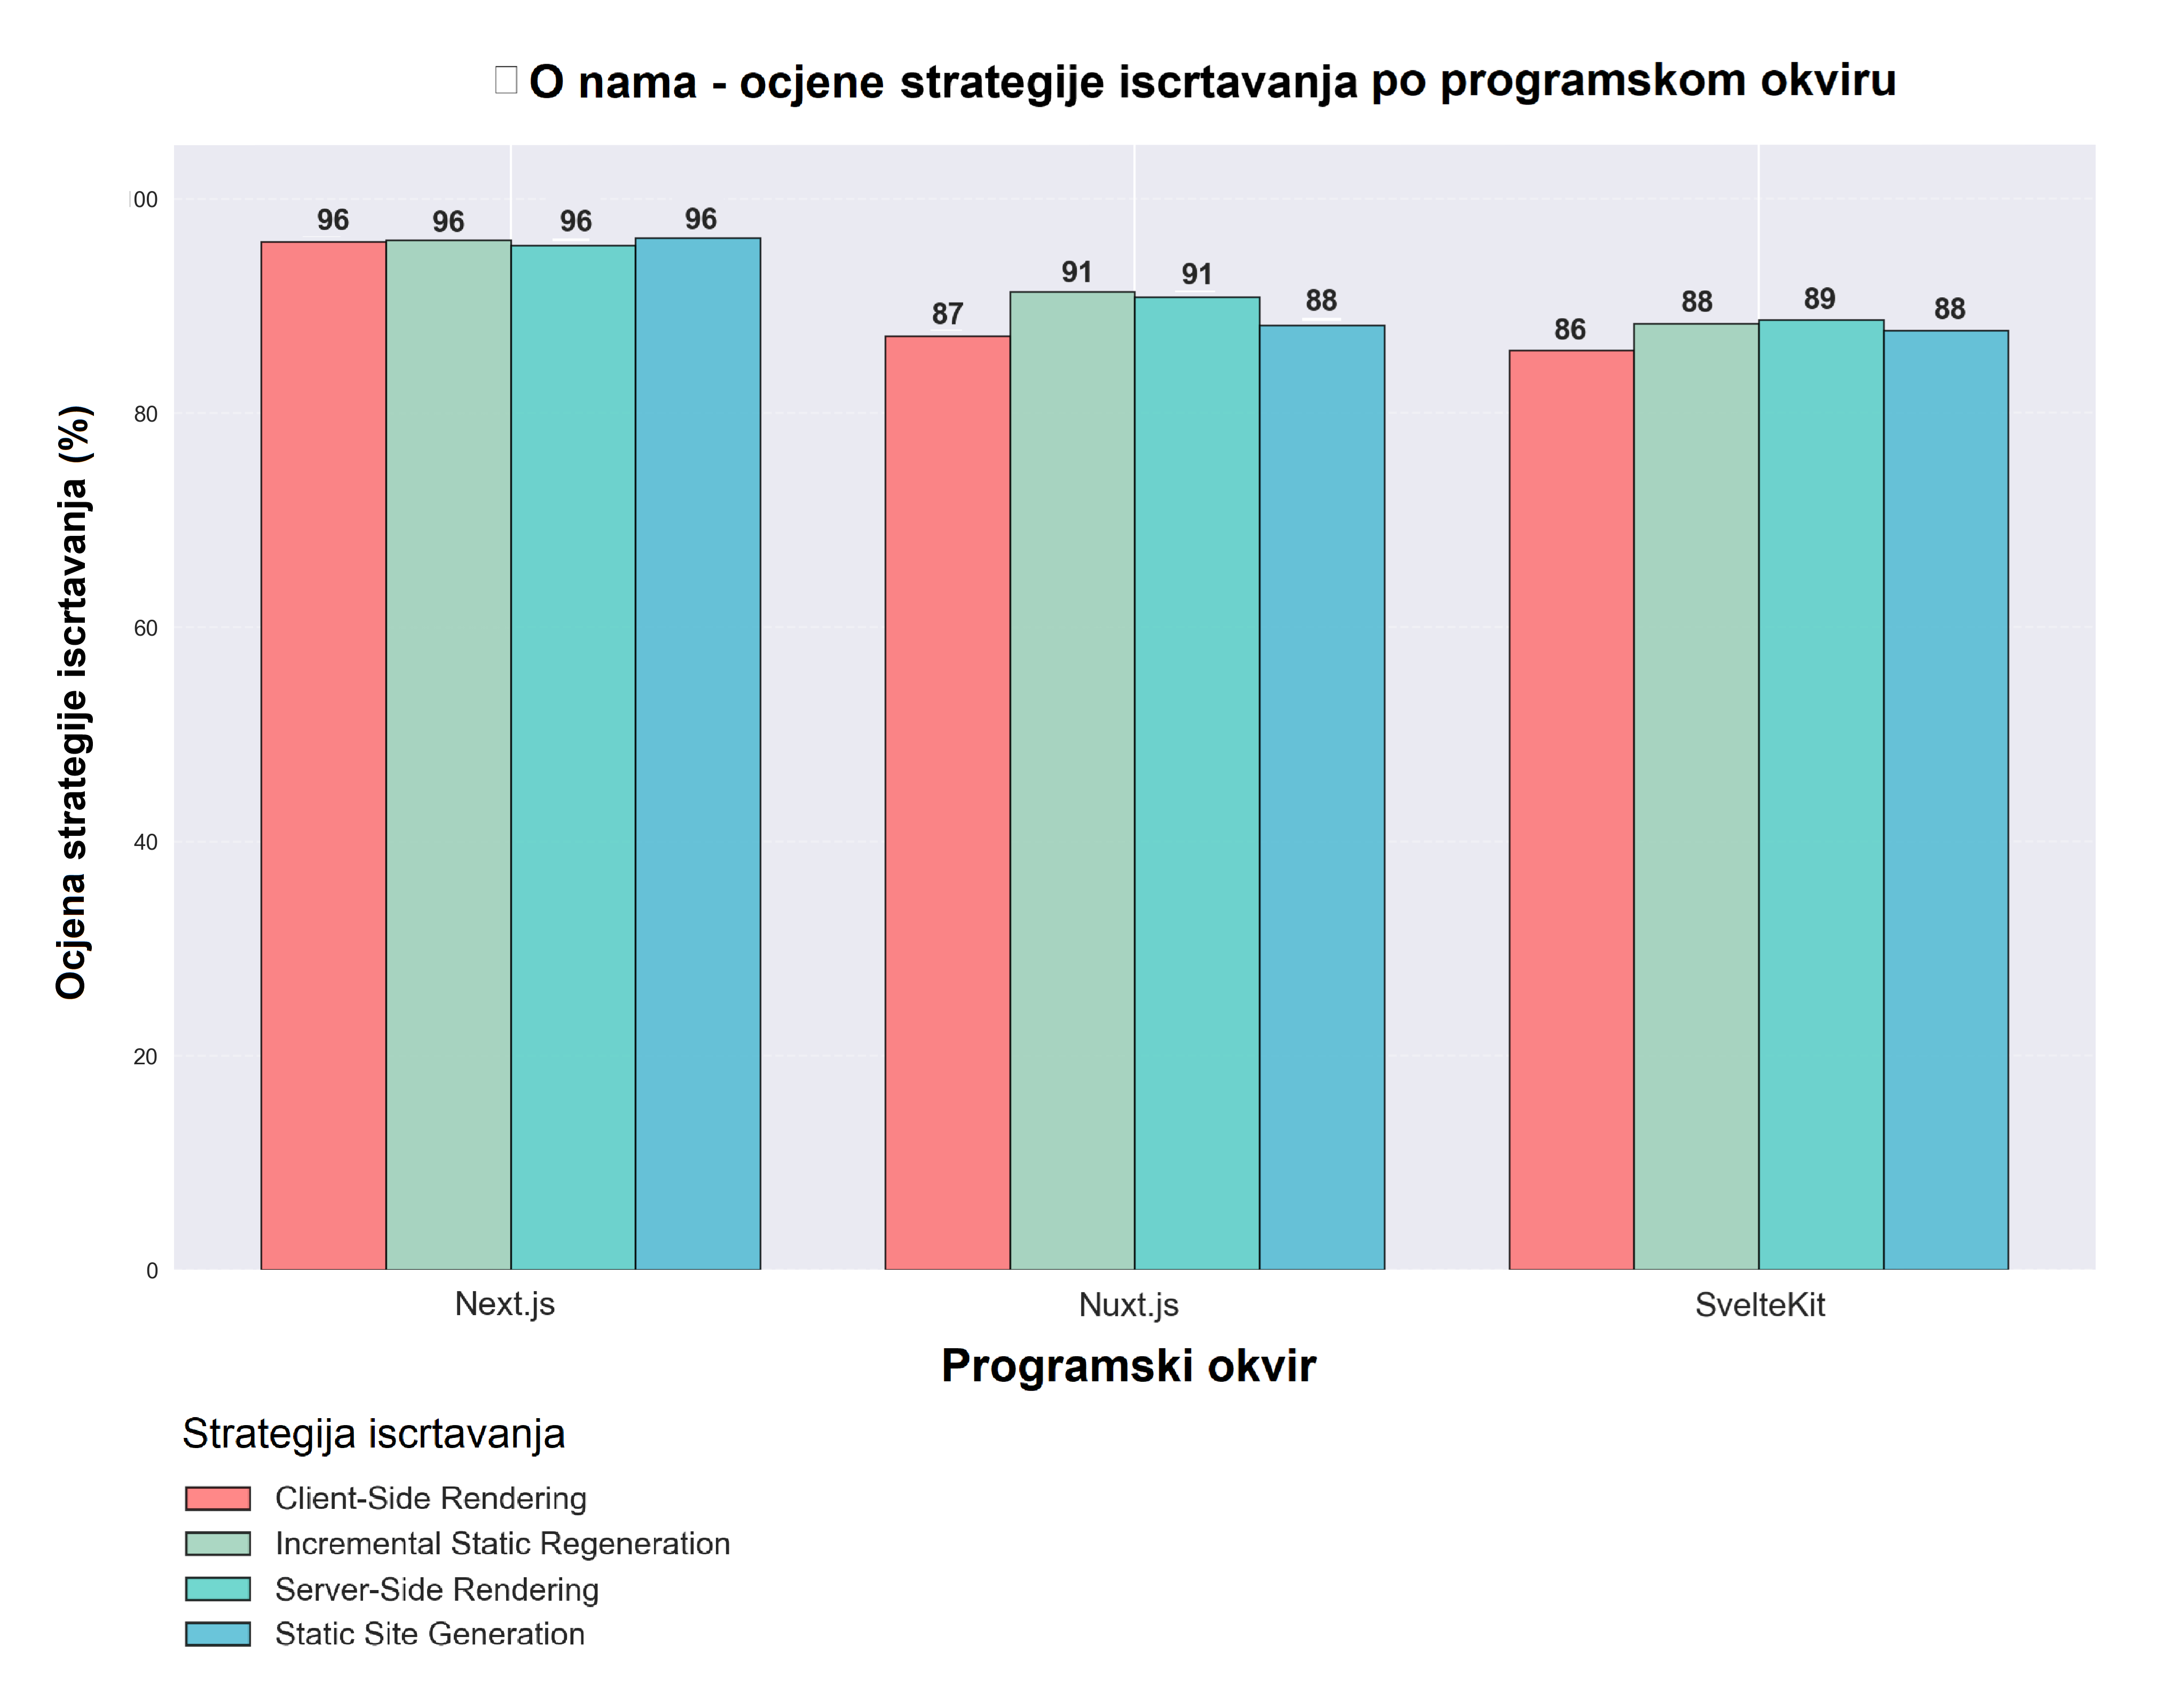
\includegraphics[width=\textwidth]{slike/rezultati/about/about_strategy_comparison.png}
    \caption{Performanse programskih okvira - usporedba strategija (stranica O nama)}
    \label{fig:testiranje-o-nama-usporedba-strategija}
\end{figure}

\newpage

\subsection{Rangiranje programskih okvira}
\begin{enumerate}
    \item Next.js: 96.0\%
    \item Nuxt.js: 89.4\%
    \item SvelteKit: 87.6\%
\end{enumerate}

\subsection{Rangiranje strategija iscrtavanja}
\begin{enumerate}
    \item Incremental Static Regeneration: 91.9\%
    \item Server-Side Rendering: 91.7\%
    \item Static Site Generation: 90.7\%
    \item Client-Side Rendering: 89.7\%
\end{enumerate}

\subsection{Najbolje kombinacije}
\begin{enumerate}
    \item Next.js + Static Site Generation: 96.3\%
    \item Next.js + Incremental Static Regeneration: 96.2\%
    \item Next.js + Client-Side Rendering: 96.0\%
    \item Next.js + Server-Side Rendering: 95.7\%
    \item Nuxt.js + Incremental Static Regeneration: 91.3\%
\end{enumerate}

\subsection{Vodeći po metrici}
\begin{itemize}
    \item FCP: Next.js + Client-Side Rendering (100.0\%, 0.920)
    \item LCP: Nuxt.js + Client-Side Rendering (88.0\%, 2.590)
    \item SI: Next.js + Client-Side Rendering (100.0\%, 1.330)
    \item TTI: Nuxt.js + Client-Side Rendering (98.0\%, 2.590)
    \item TBT: Next.js + Client-Side Rendering (100.0\%, 8.200)
    \item CLS: Next.js + Client-Side Rendering (100.0\%, 0.000)
\end{itemize}



\newpage

\section{Rezultati}

\subsection{Stranica Blog}

\begin{figure}[H]
    \centering
    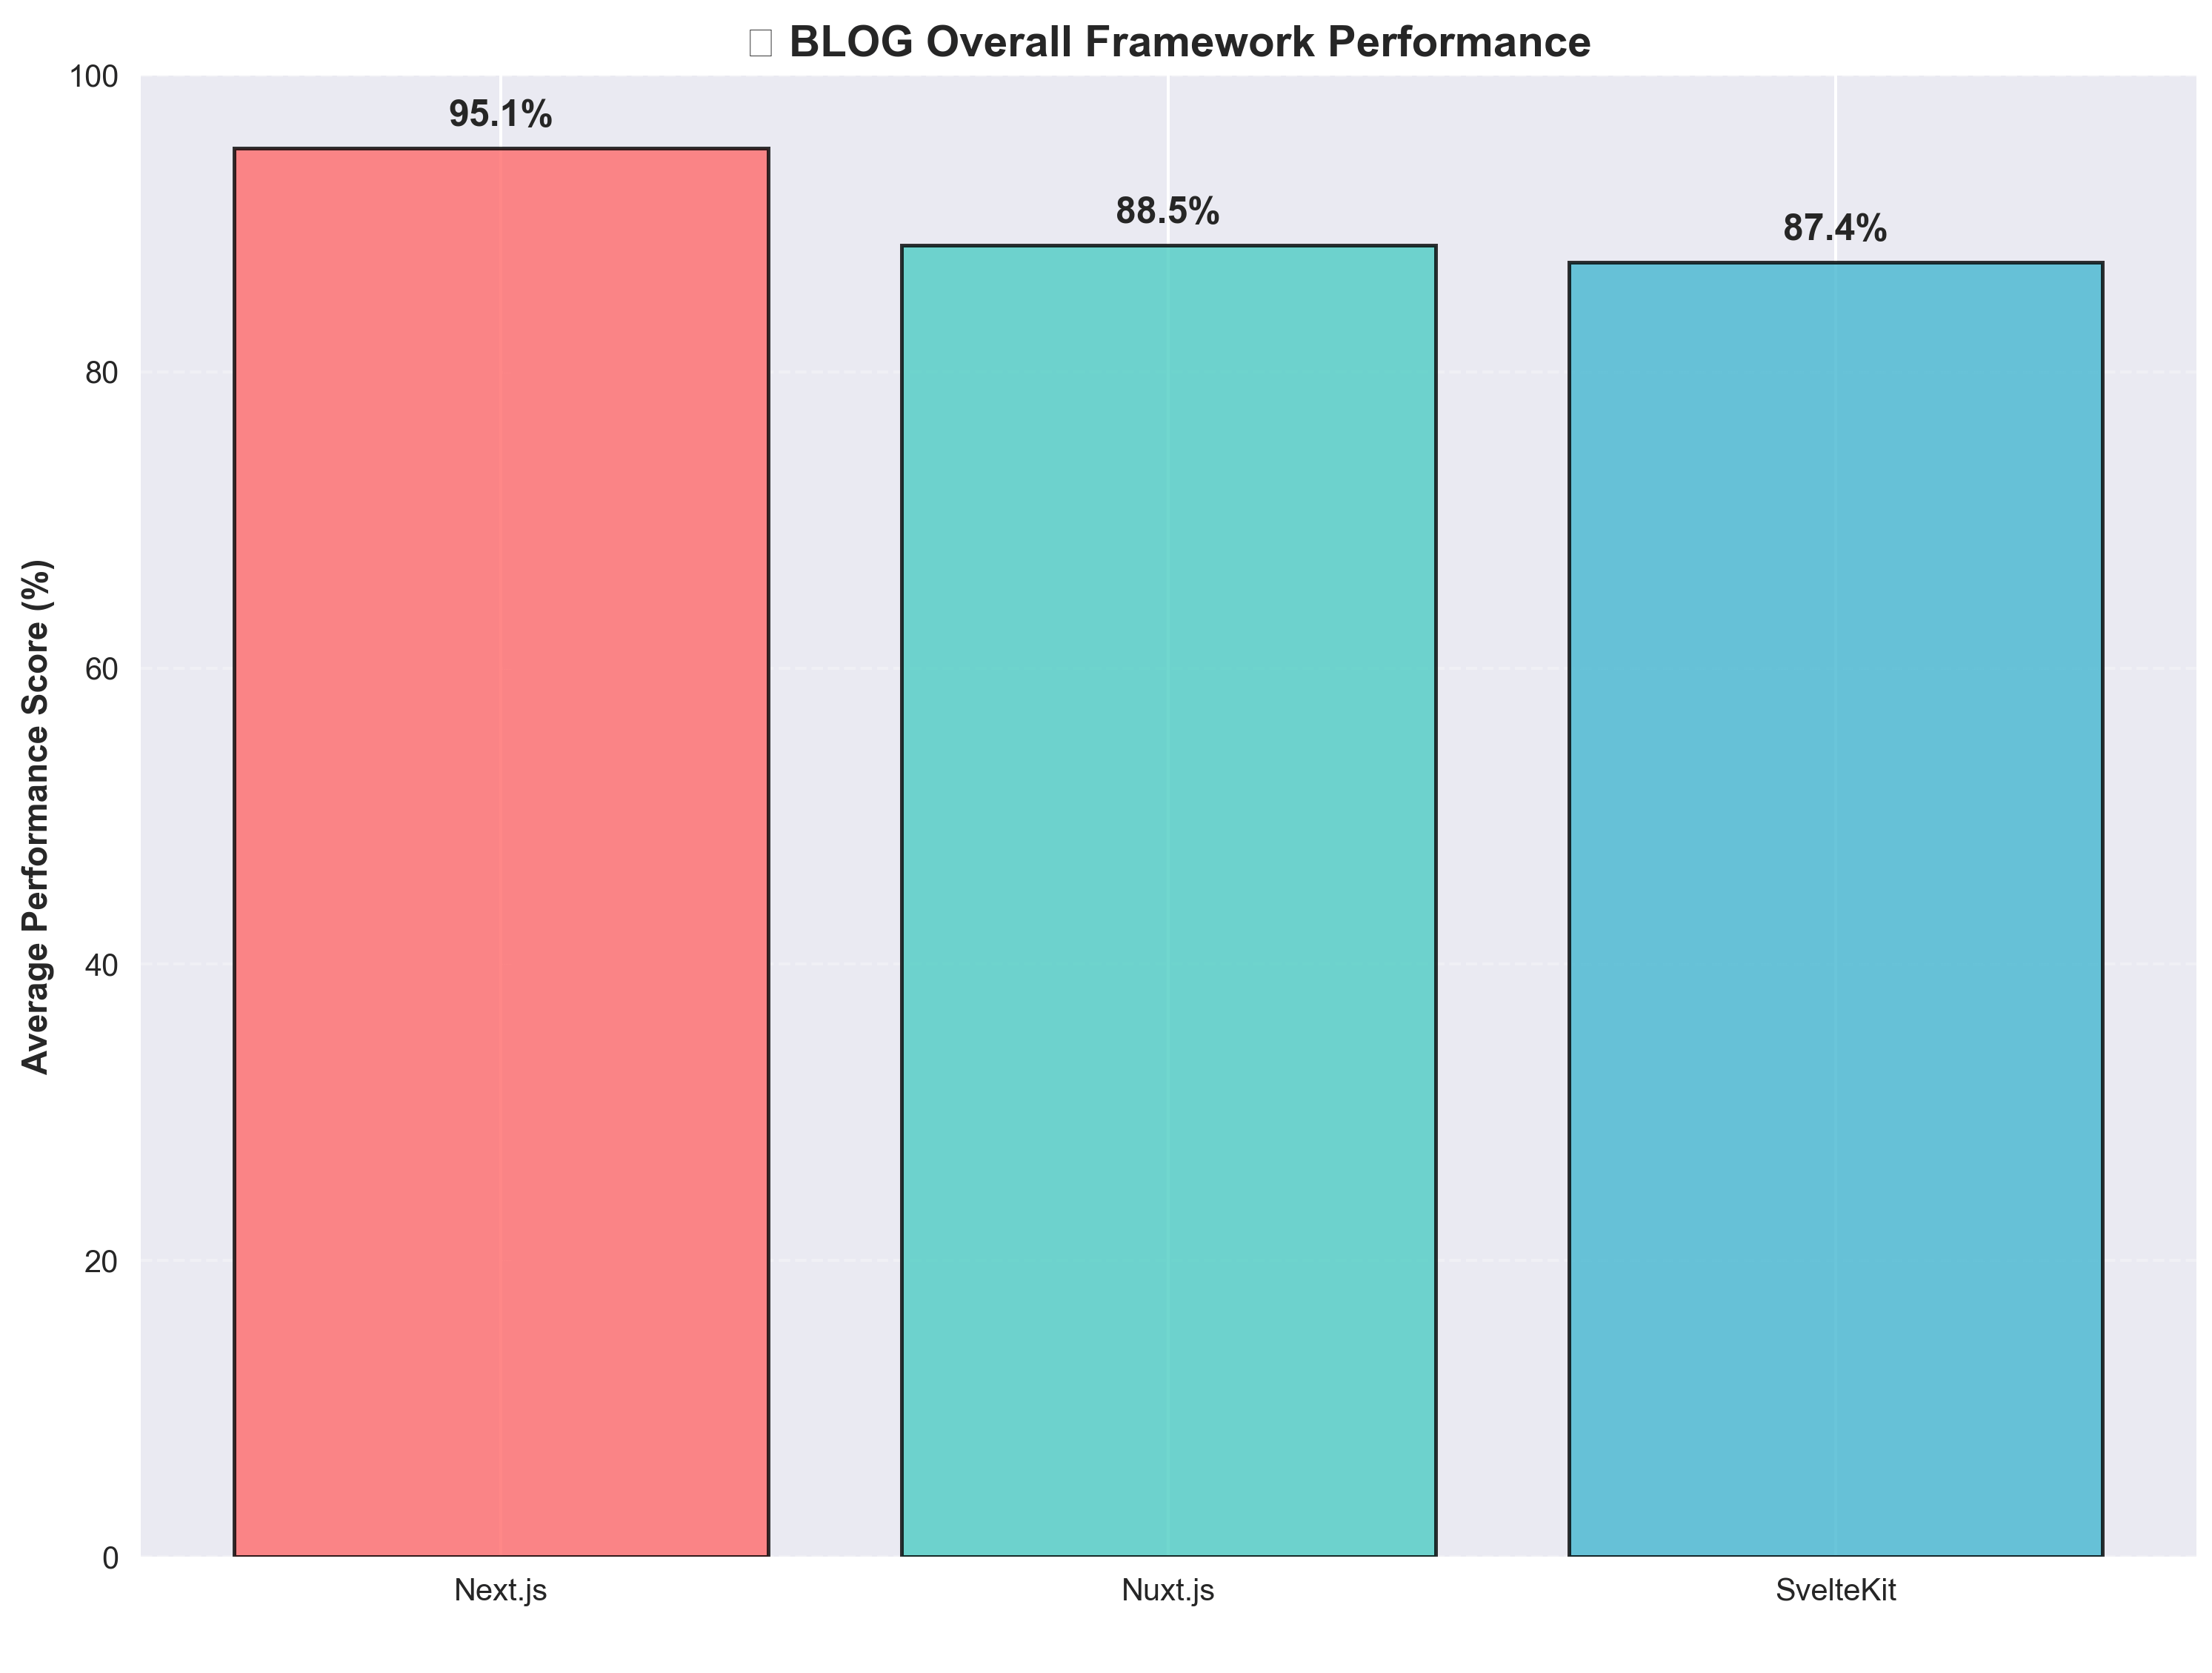
\includegraphics[width=0.8\textwidth]{slike/rezultati/blog/blog_framework_overall_performance.png}
    \caption{Ukupne performanse programskih okvira}
    \label{fig:testiranje-blog-ukupne-performanse}
\end{figure}

\begin{figure}[H]
    \centering
    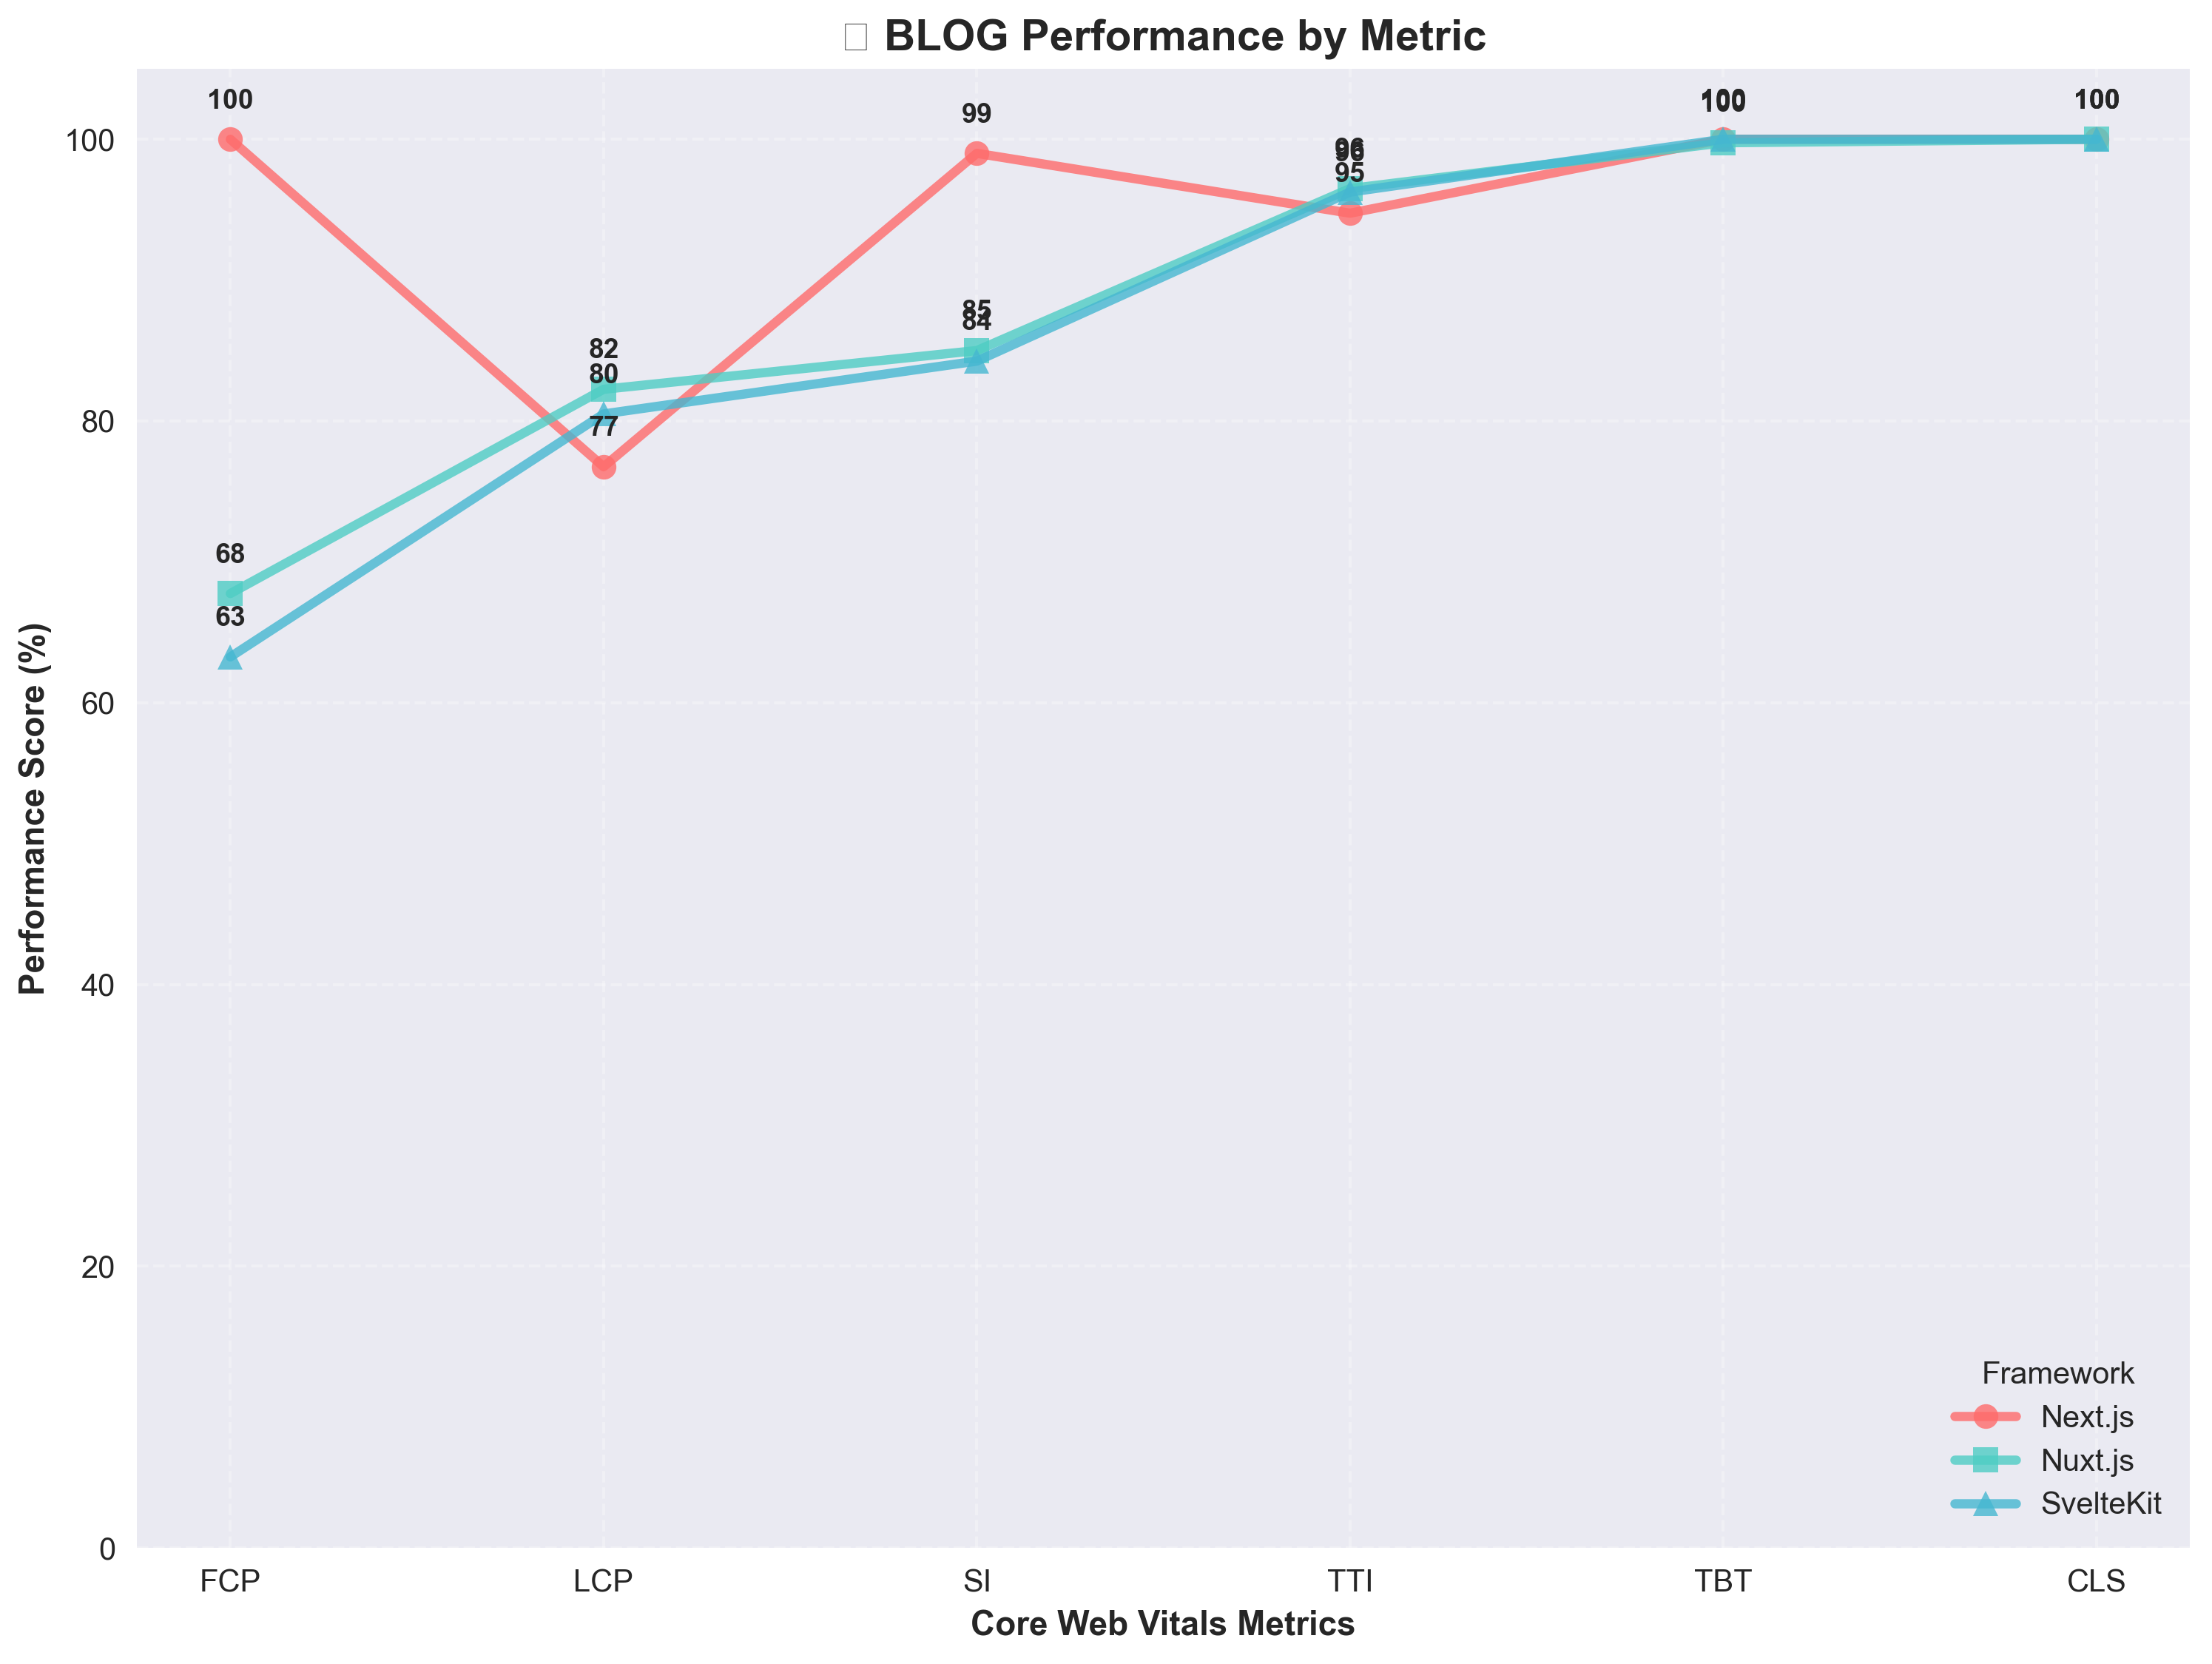
\includegraphics[width=0.8\textwidth]{slike/rezultati/blog/blog_performance_by_metric.png}
    \caption{Ukupne performanse programskih okvira po metrici}
    \label{fig:testiranje-blog-performanse-po-metrici}
\end{figure}

\begin{figure}[H]
    \centering
    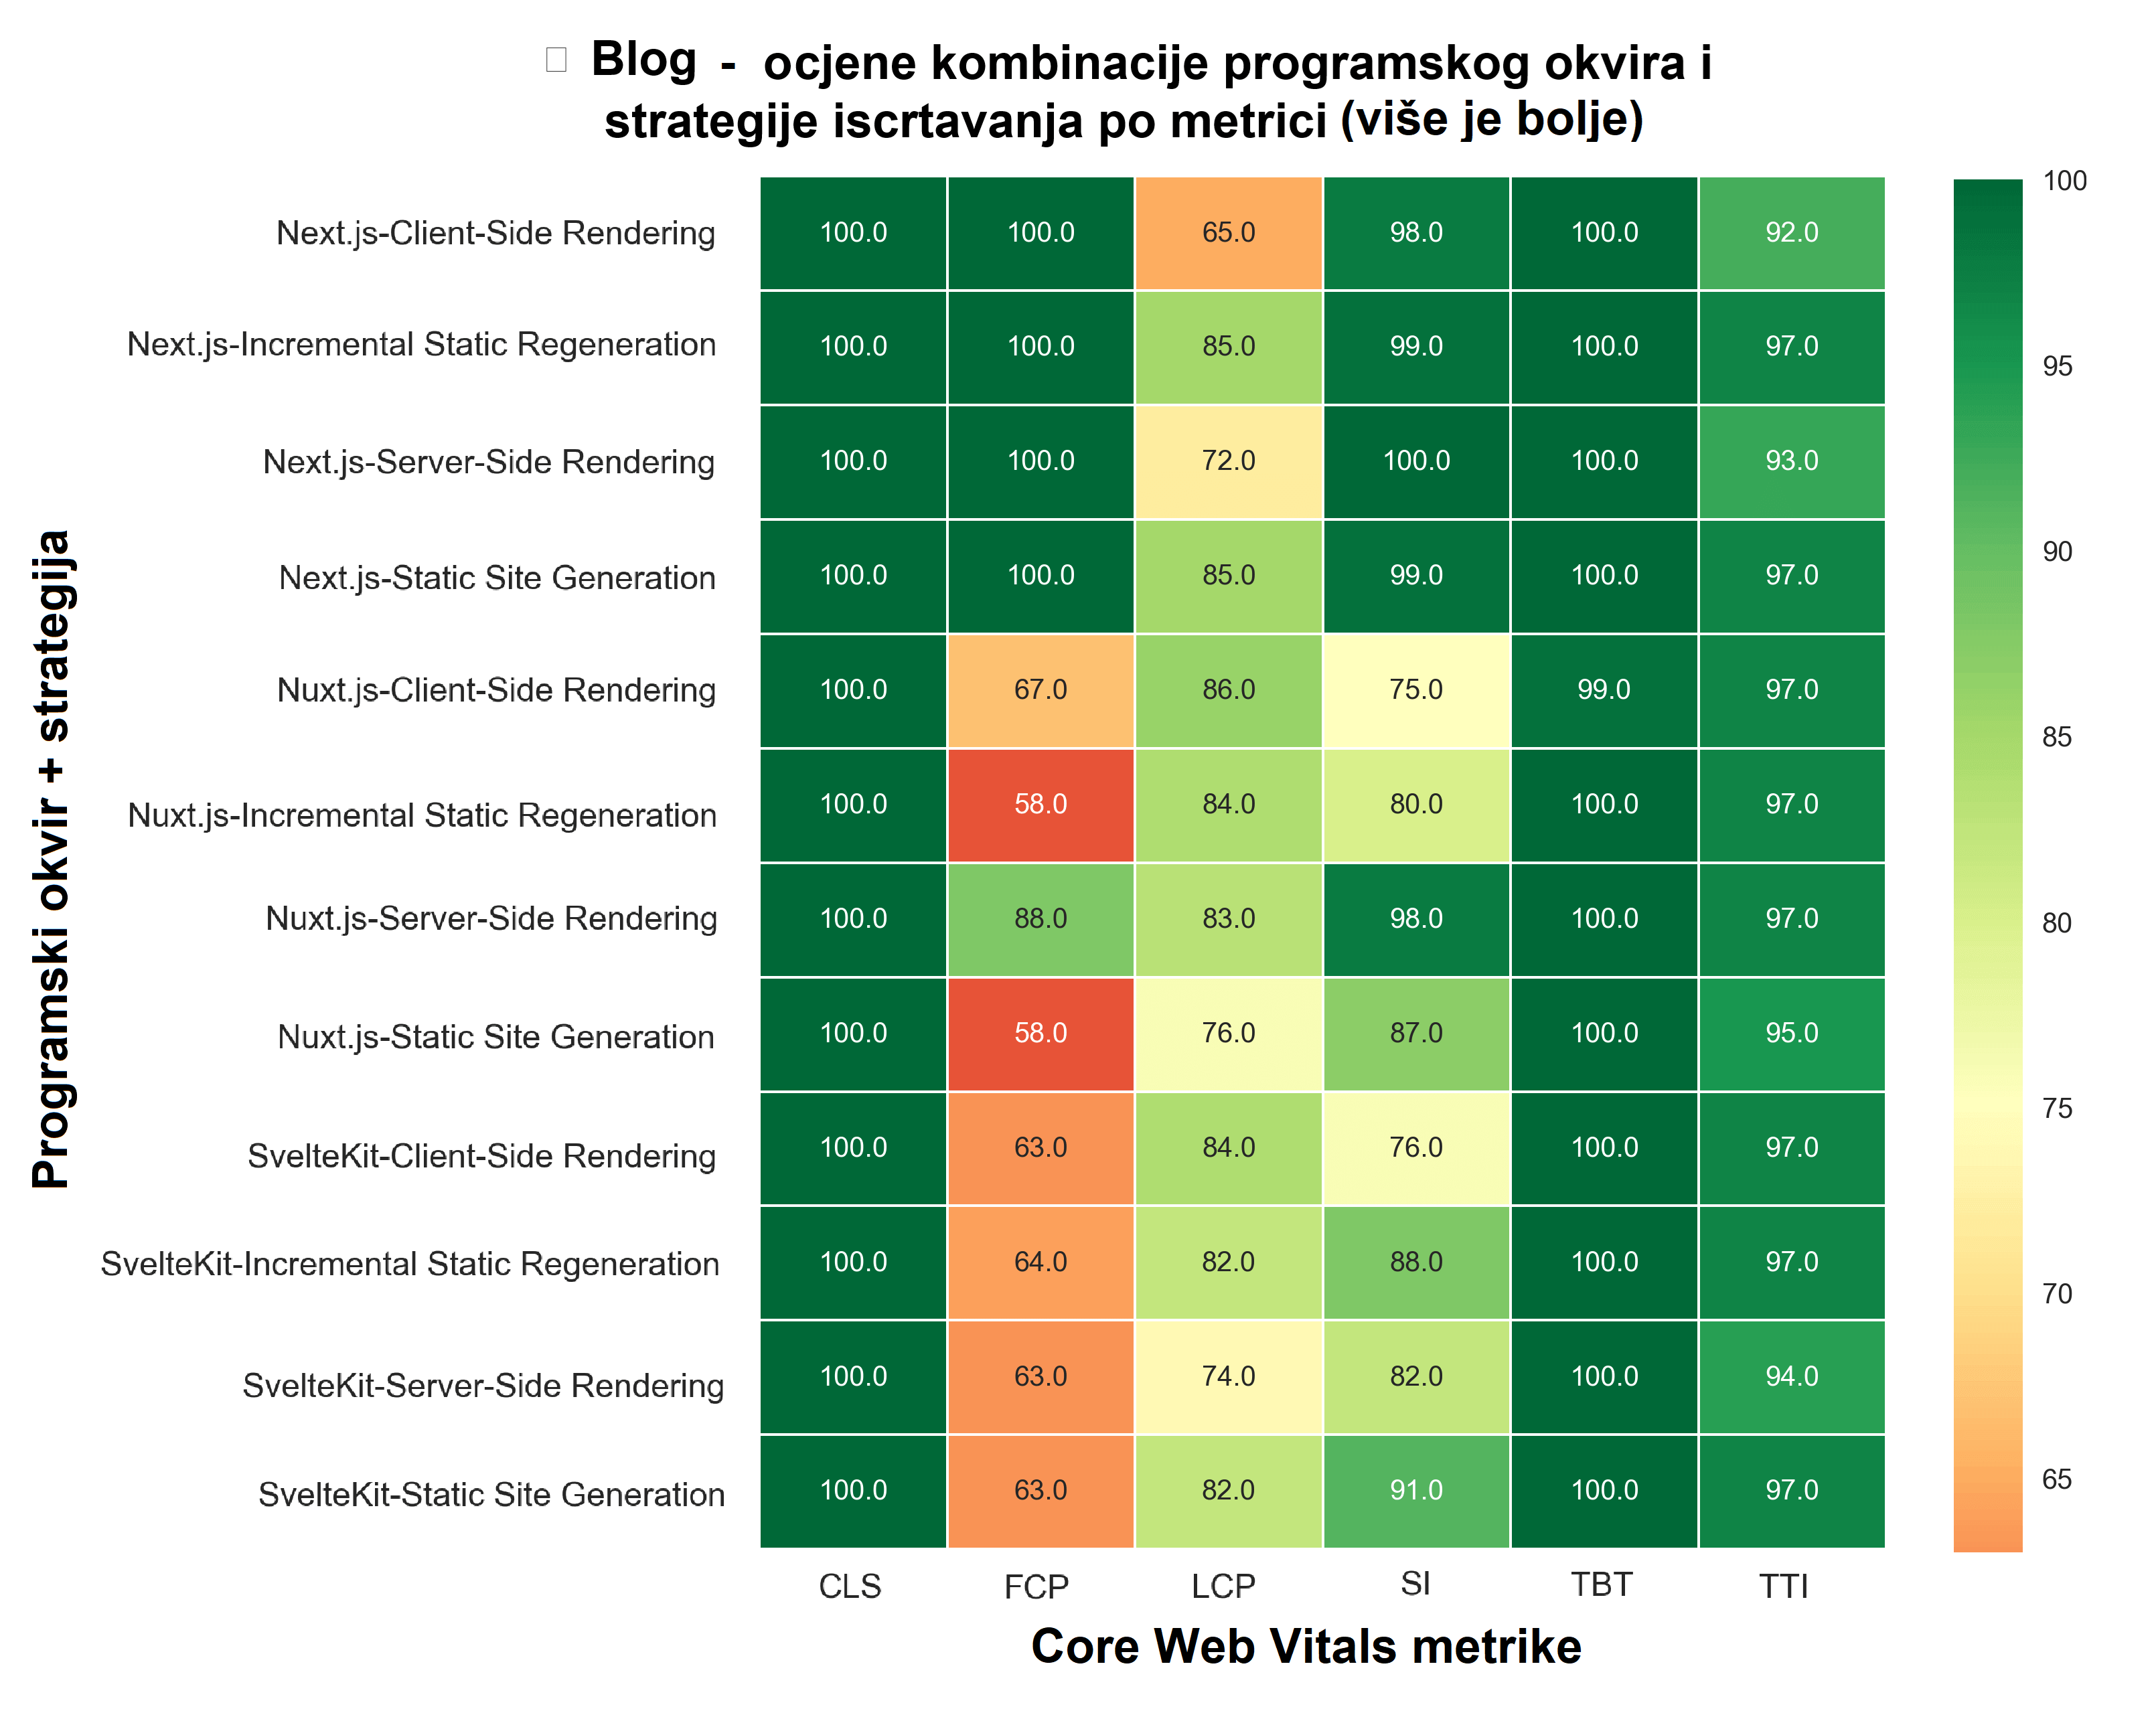
\includegraphics[width=\textwidth]{slike/rezultati/blog/blog_performance_scores.png}
    \caption{Performanse programskih okvira - postotak}
    \label{fig:testiranje-blog-postotak}
\end{figure}

\begin{figure}[H]
    \centering
    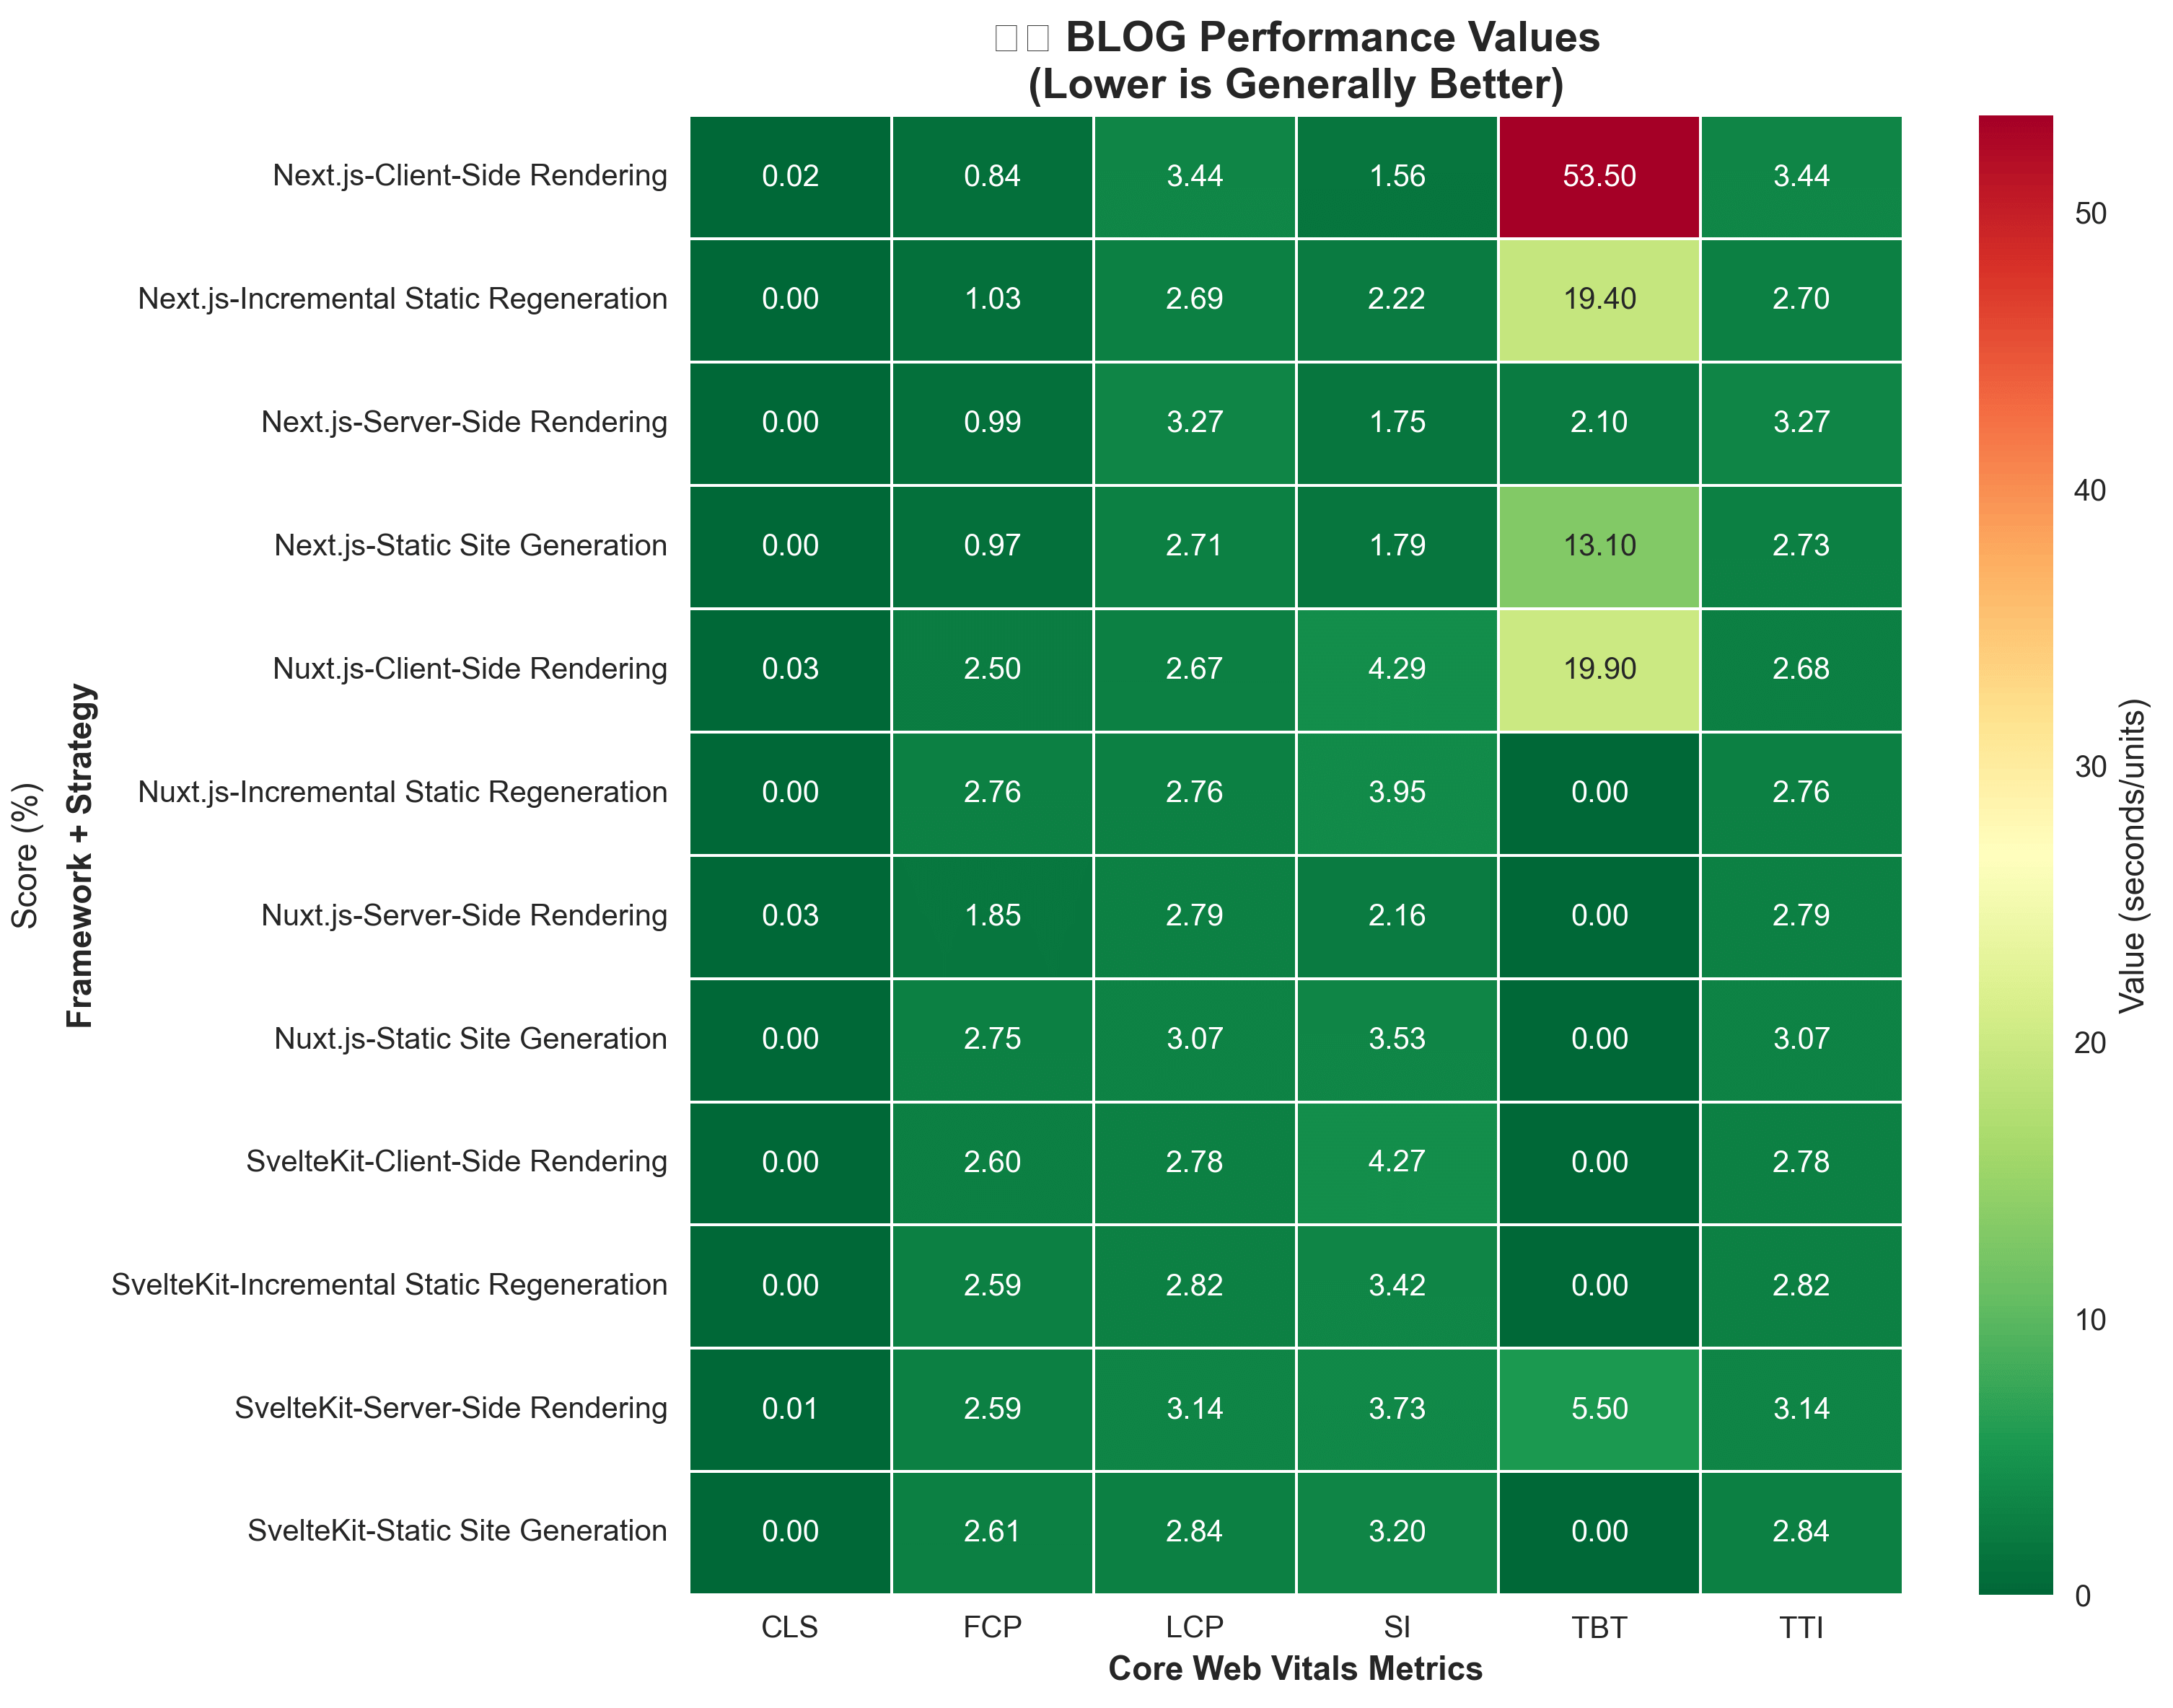
\includegraphics[width=\textwidth]{slike/rezultati/blog/blog_performance_values.png}
    \caption{Performanse programskih okvira - vrijednosti}
    \label{fig:testiranje-blog-vrijednosti}
\end{figure}

\begin{figure}[H]
    \centering
    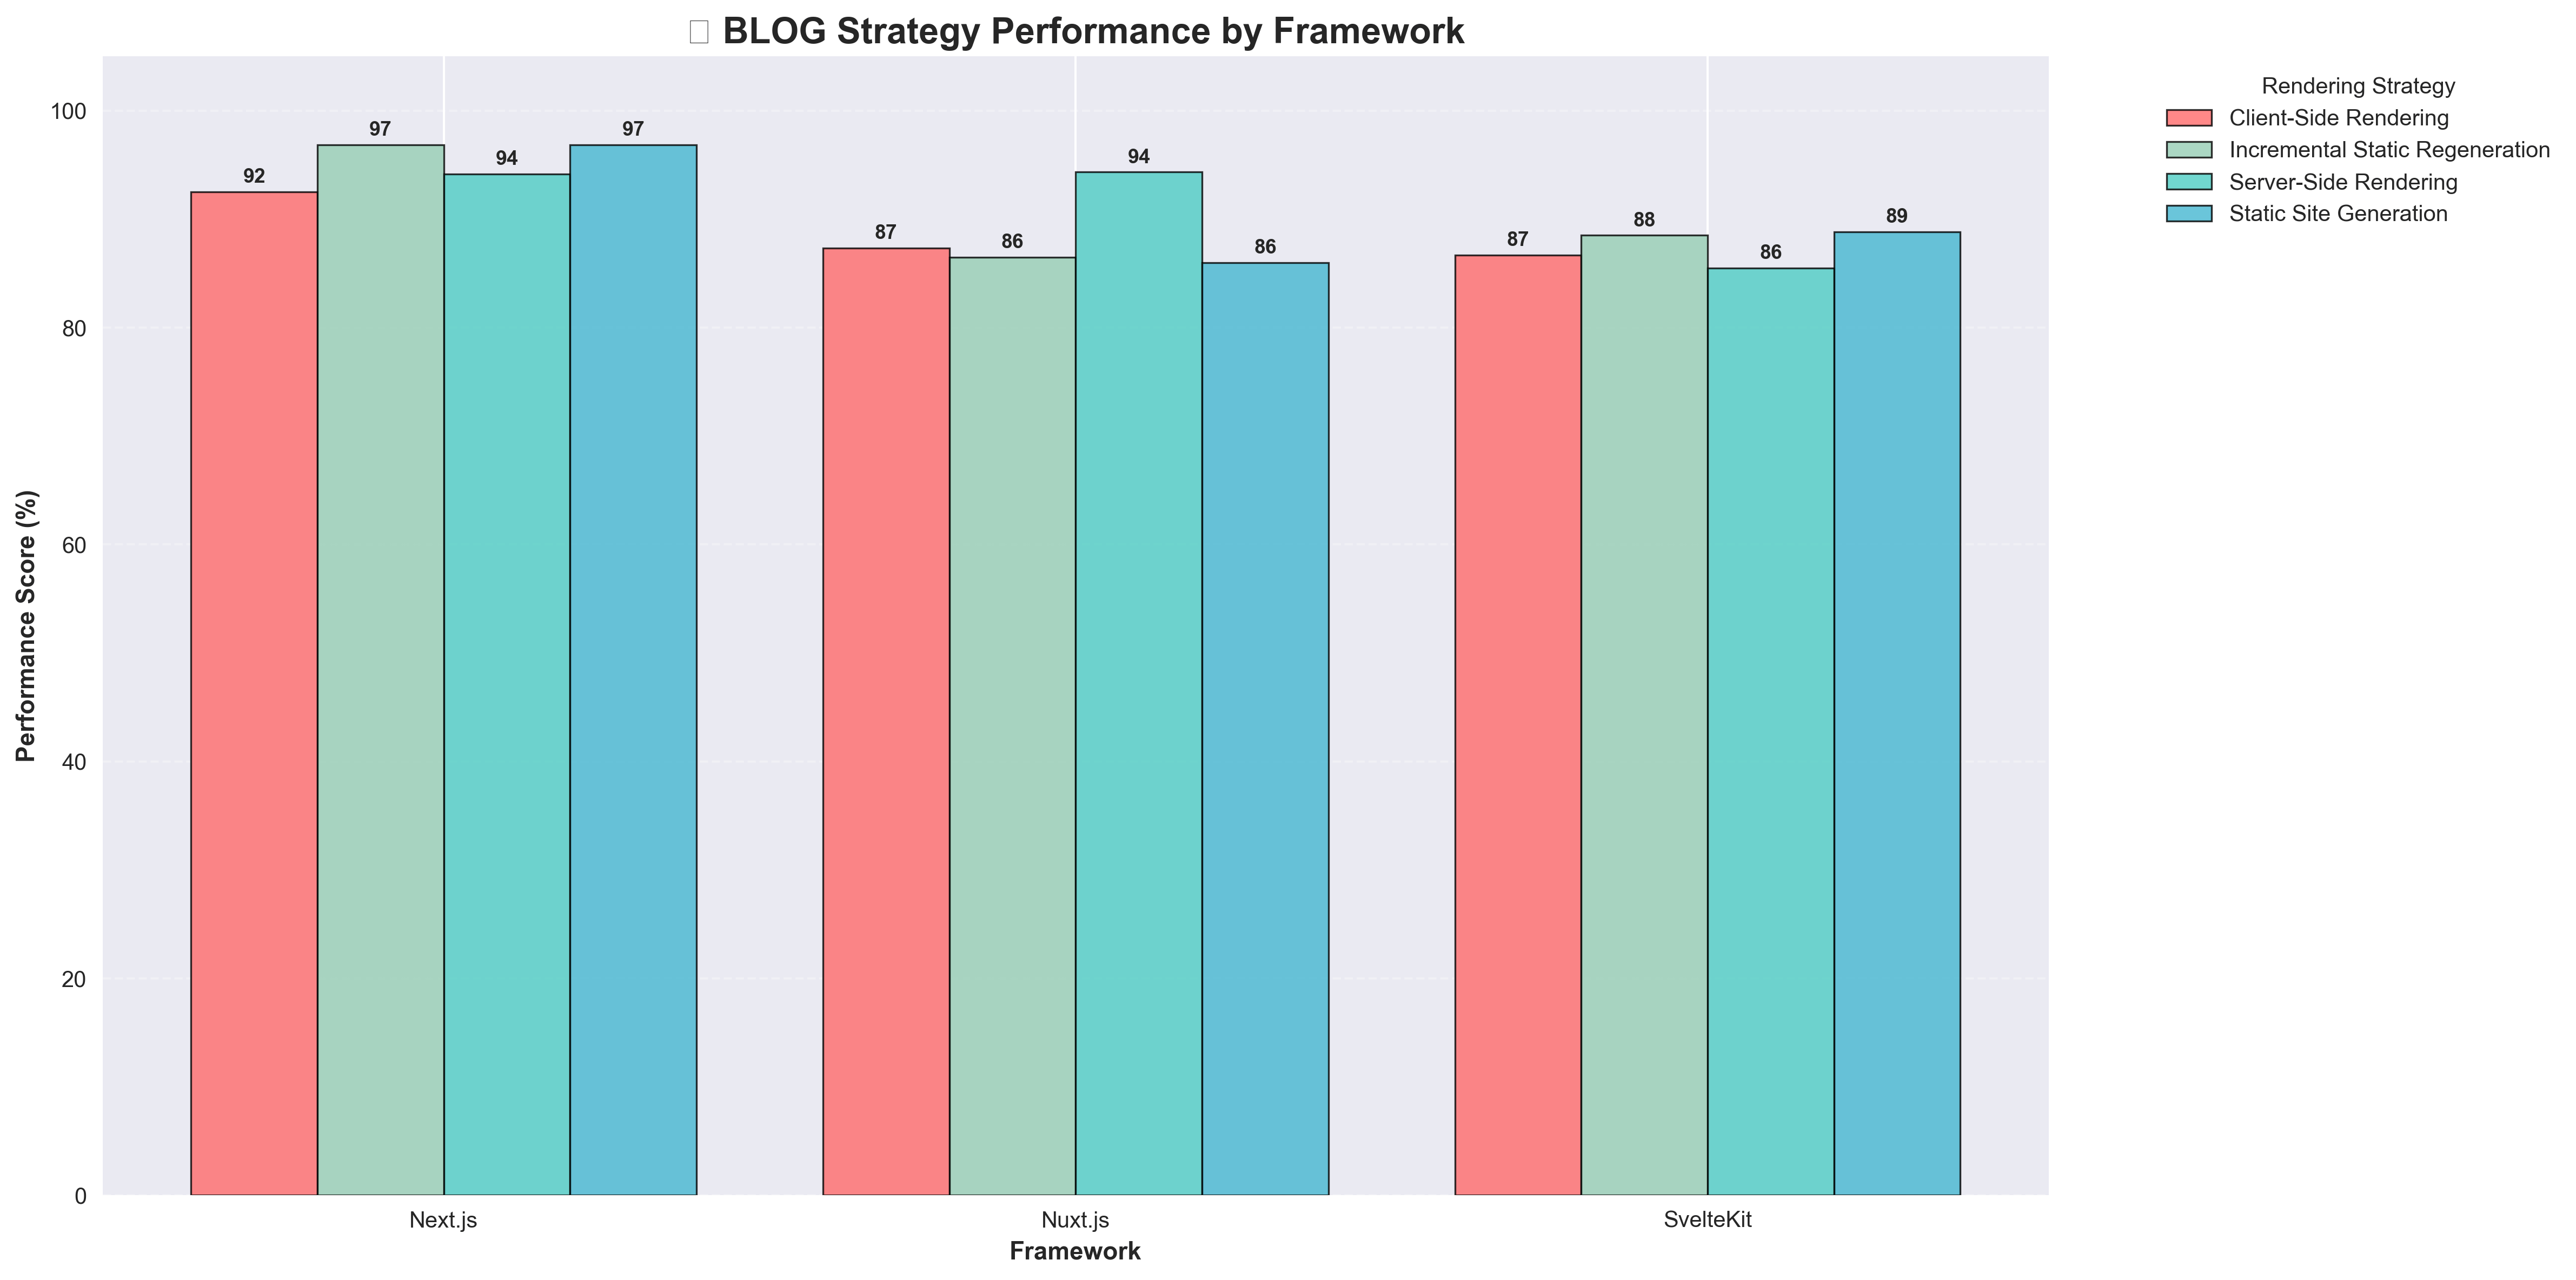
\includegraphics[width=\textwidth]{slike/rezultati/blog/blog_strategy_comparison.png}
    \caption{Performanse programskih okvira - usporedba strategija}
    \label{fig:testiranje-blog-usporedba-strategija}
\end{figure}

\subsubsection{Rangiranje programskih okvira}
\begin{enumerate}
    \item Next.js: 96.0\%
    \item Nuxt.js: 89.4\%
    \item SvelteKit: 87.6\%
\end{enumerate}

\subsubsection{Rangiranje strategija iscrtavanja}
\begin{enumerate}
    \item Incremental Static Regeneration: 91.9\%
    \item Server-Side Rendering: 91.7\%
    \item Static Site Generation: 90.7\%
    \item Client-Side Rendering: 89.7\%
\end{enumerate}

\subsubsection{Najbolje kombinacije}
\begin{enumerate}
    \item Next.js + Static Site Generation: 96.3\%
    \item Next.js + Incremental Static Regeneration: 96.2\%
    \item Next.js + Client-Side Rendering: 96.0\%
    \item Next.js + Server-Side Rendering: 95.7\%
    \item Nuxt.js + Incremental Static Regeneration: 91.3\%
\end{enumerate}

\subsubsection{Vodeći po metrici}
\begin{itemize}
    \item FCP: Next.js + Client-Side Rendering (100.0\%, 0.920)
    \item LCP: Nuxt.js + Client-Side Rendering (88.0\%, 2.590)
    \item SI: Next.js + Client-Side Rendering (100.0\%, 1.330)
    \item TTI: Nuxt.js + Client-Side Rendering (98.0\%, 2.590)
    \item TBT: Next.js + Client-Side Rendering (100.0\%, 8.200)
    \item CLS: Next.js + Client-Side Rendering (100.0\%, 0.000)
\end{itemize}


\newpage


\subsection{Stranica pojedinog bloga}

\begin{figure}[H]
    \centering
    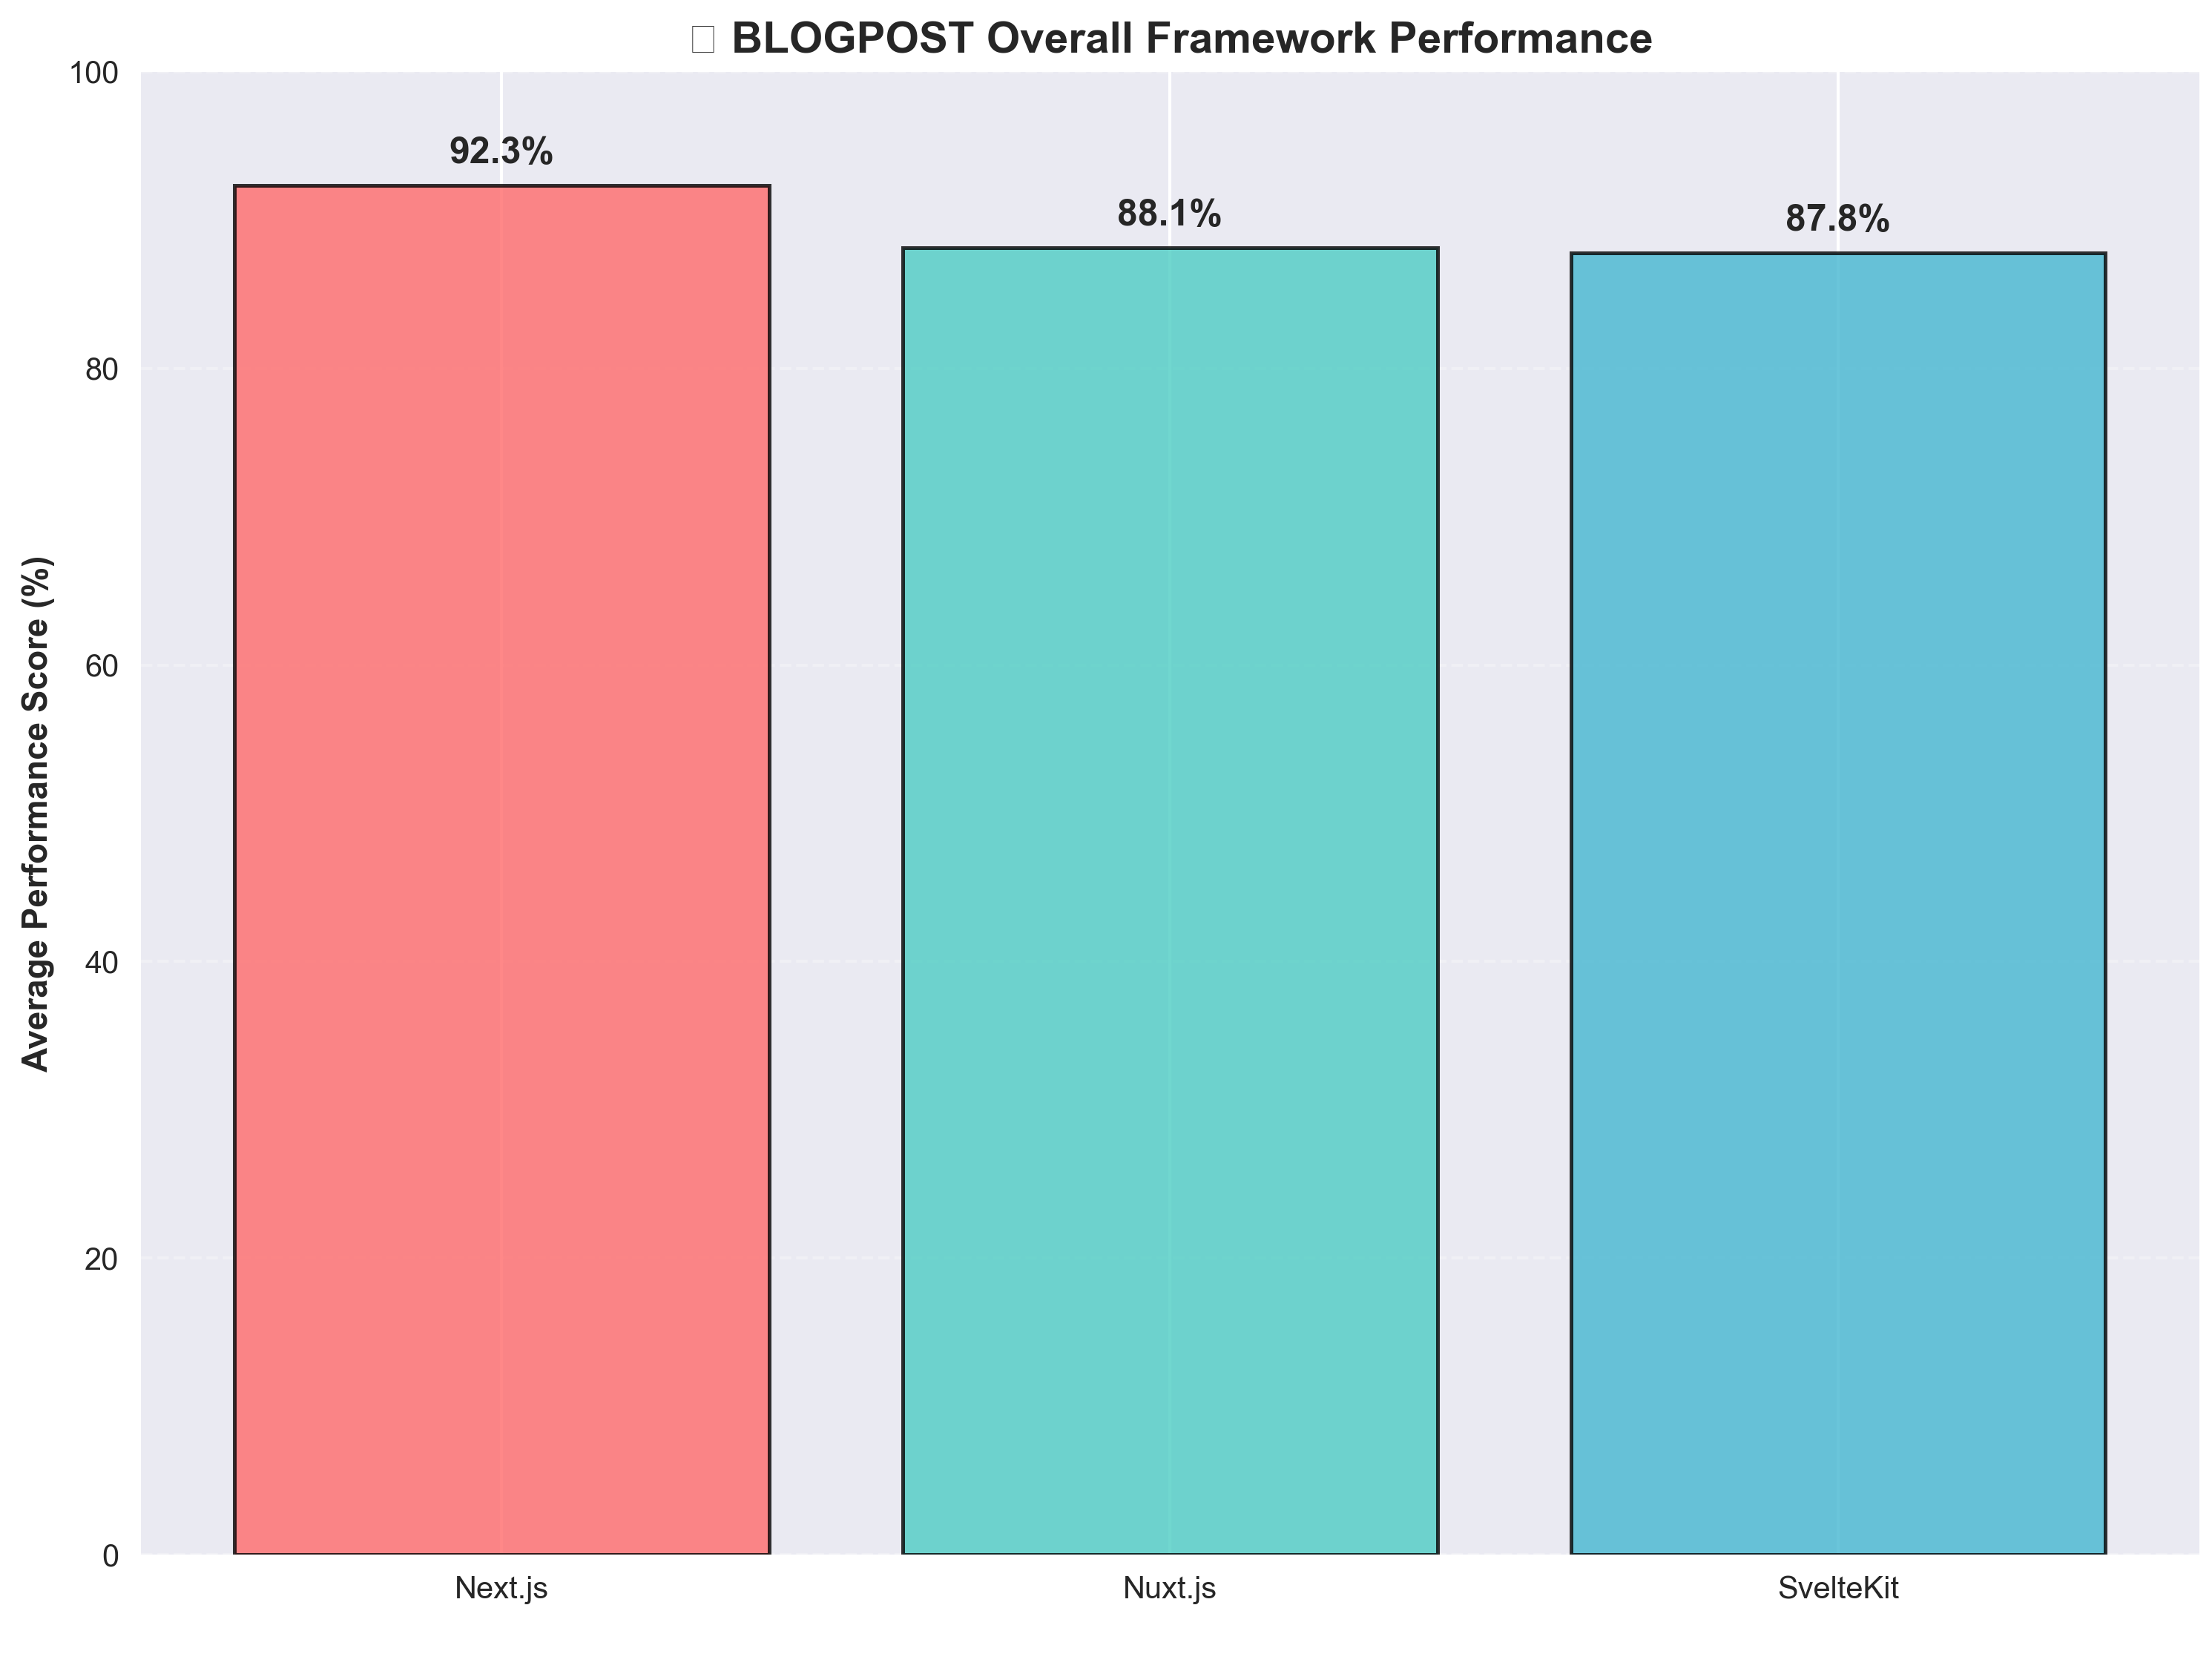
\includegraphics[width=0.8\textwidth]{slike/rezultati/blog-post/blogPost_framework_overall_performance.png}
    \caption{Ukupne ocjene radnih značajki (stranica pojedinog bloga) }
    \label{fig:testiranje-blog-post-ukupne-performanse}
\end{figure}

\begin{figure}[H]
    \centering
    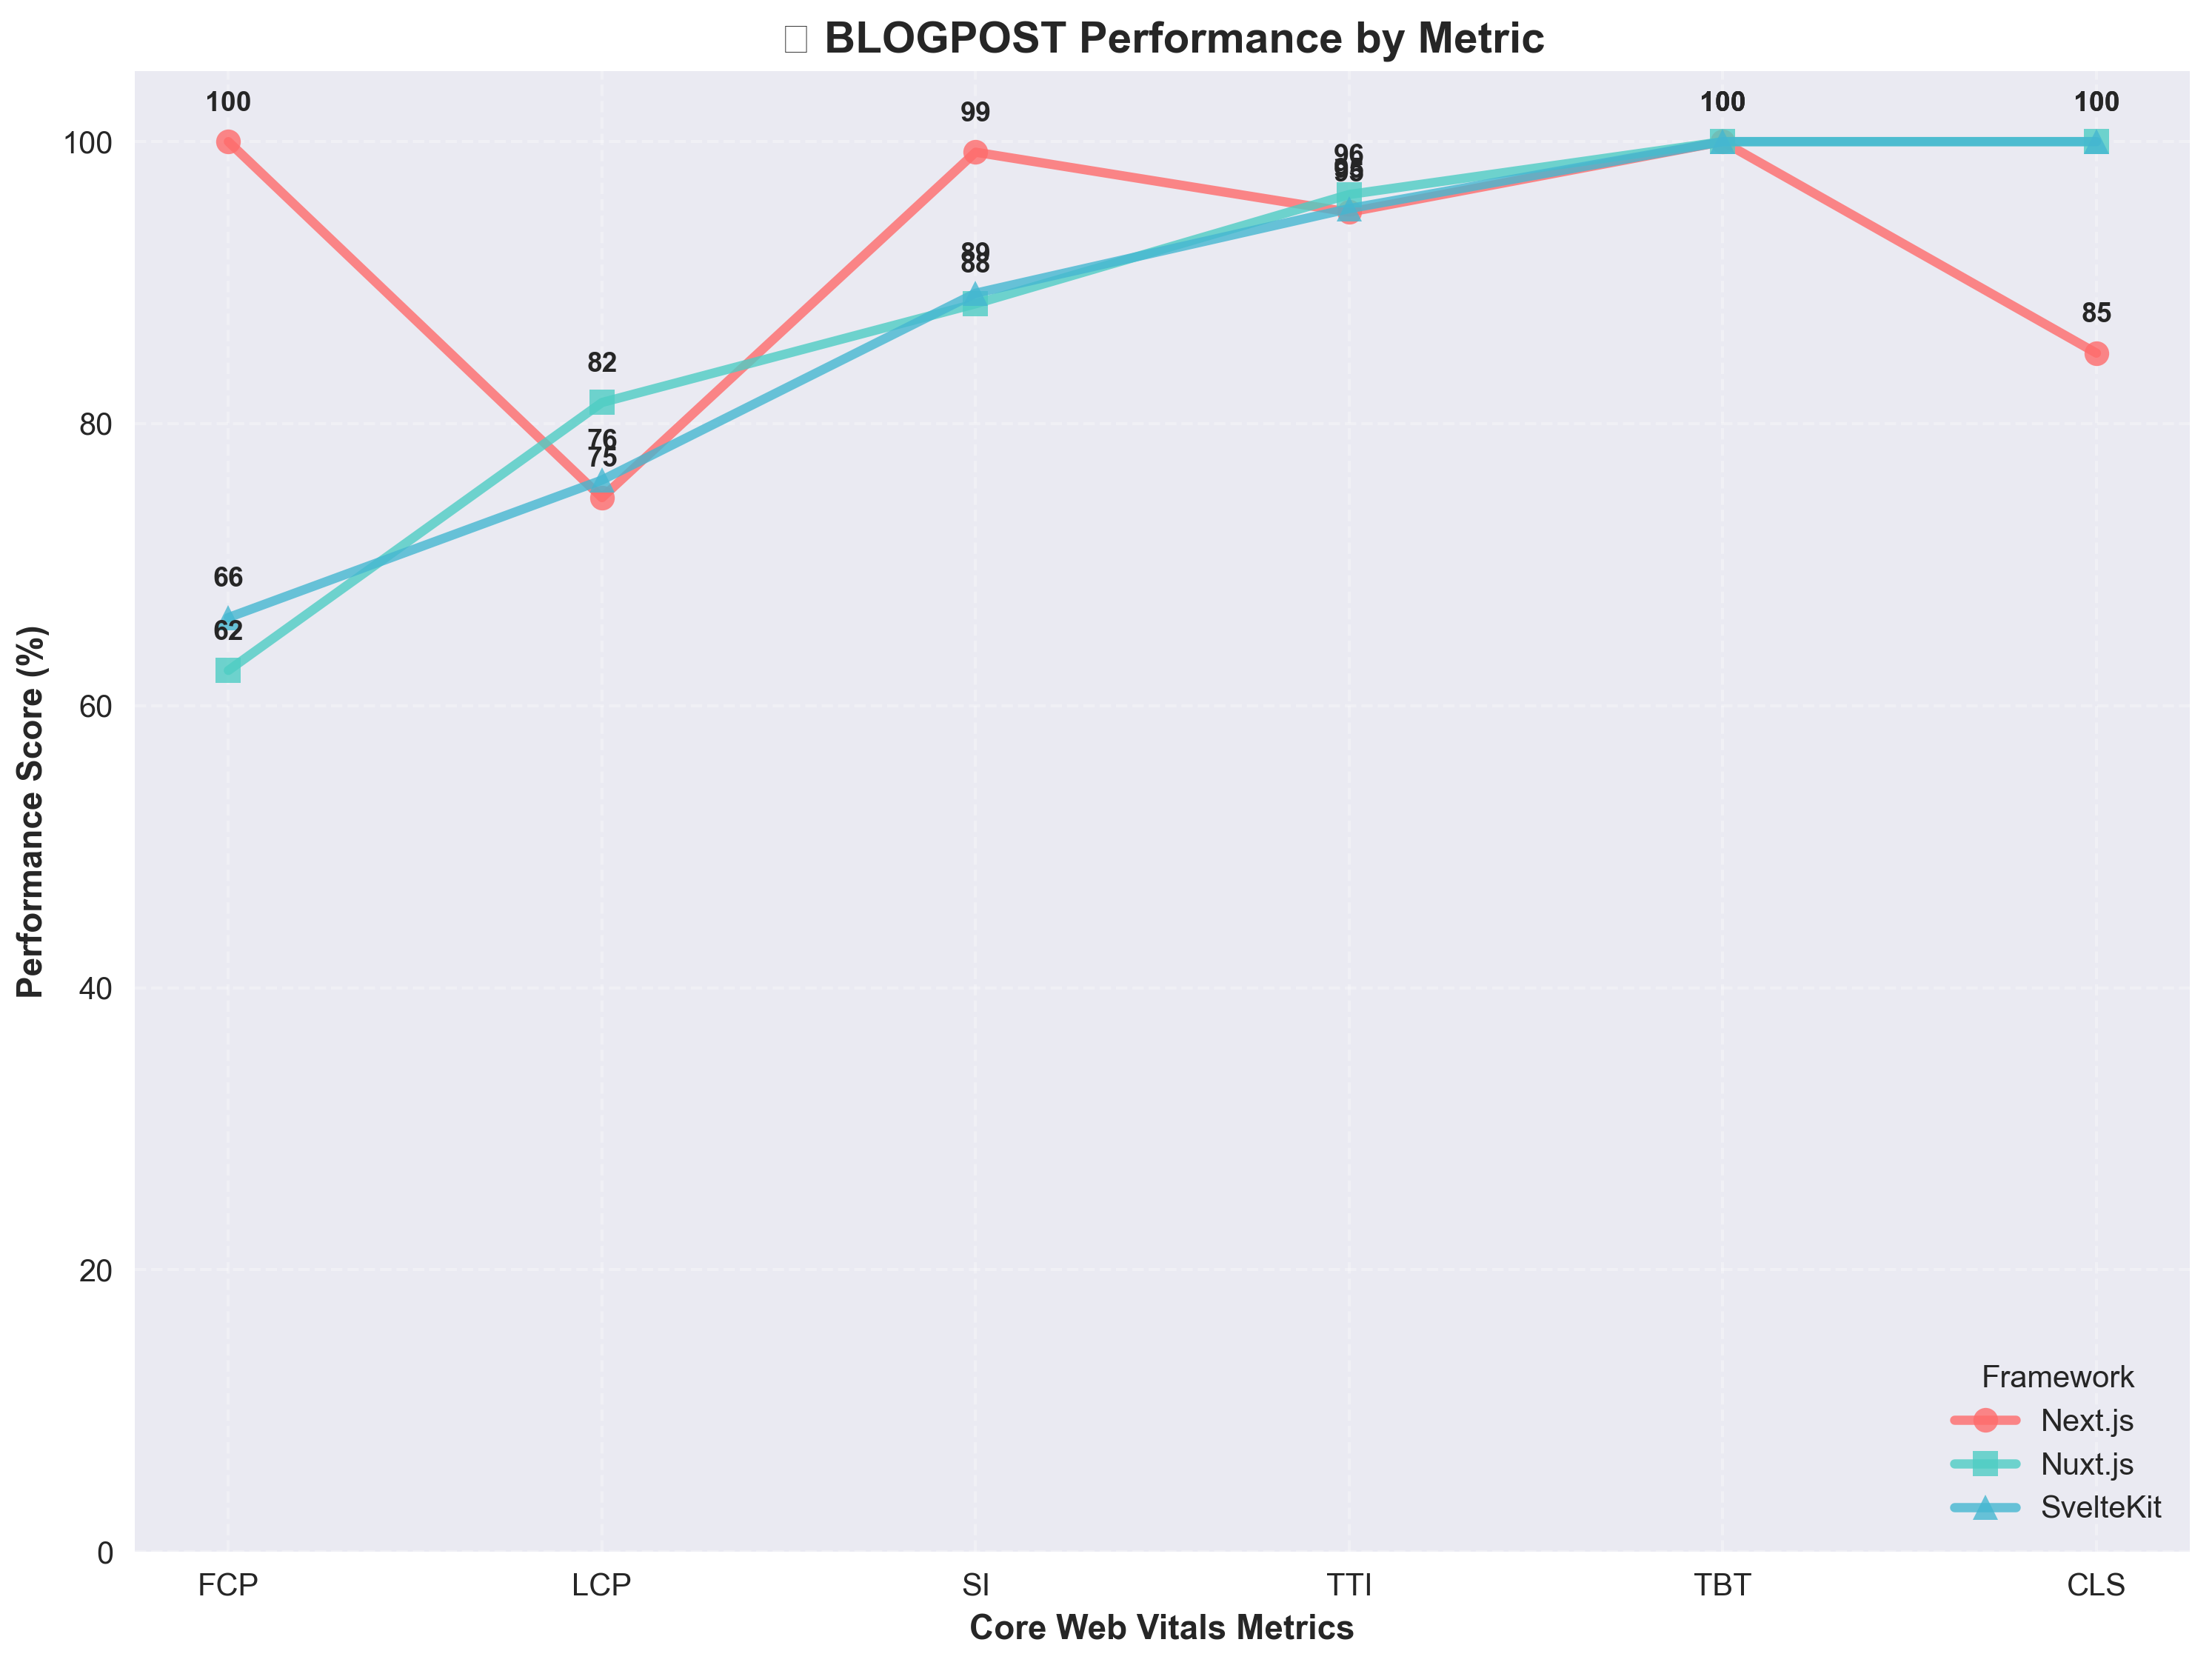
\includegraphics[width=0.8\textwidth]{slike/rezultati/blog-post/blogPost_performance_by_metric.png}
    \caption{Ukupne ocjene radnih značajki po metrici (stranica pojedinog bloga) }
    \label{fig:testiranje-blog-post-performanse-po-metrici}
\end{figure}

\begin{figure}[H]
    \centering
    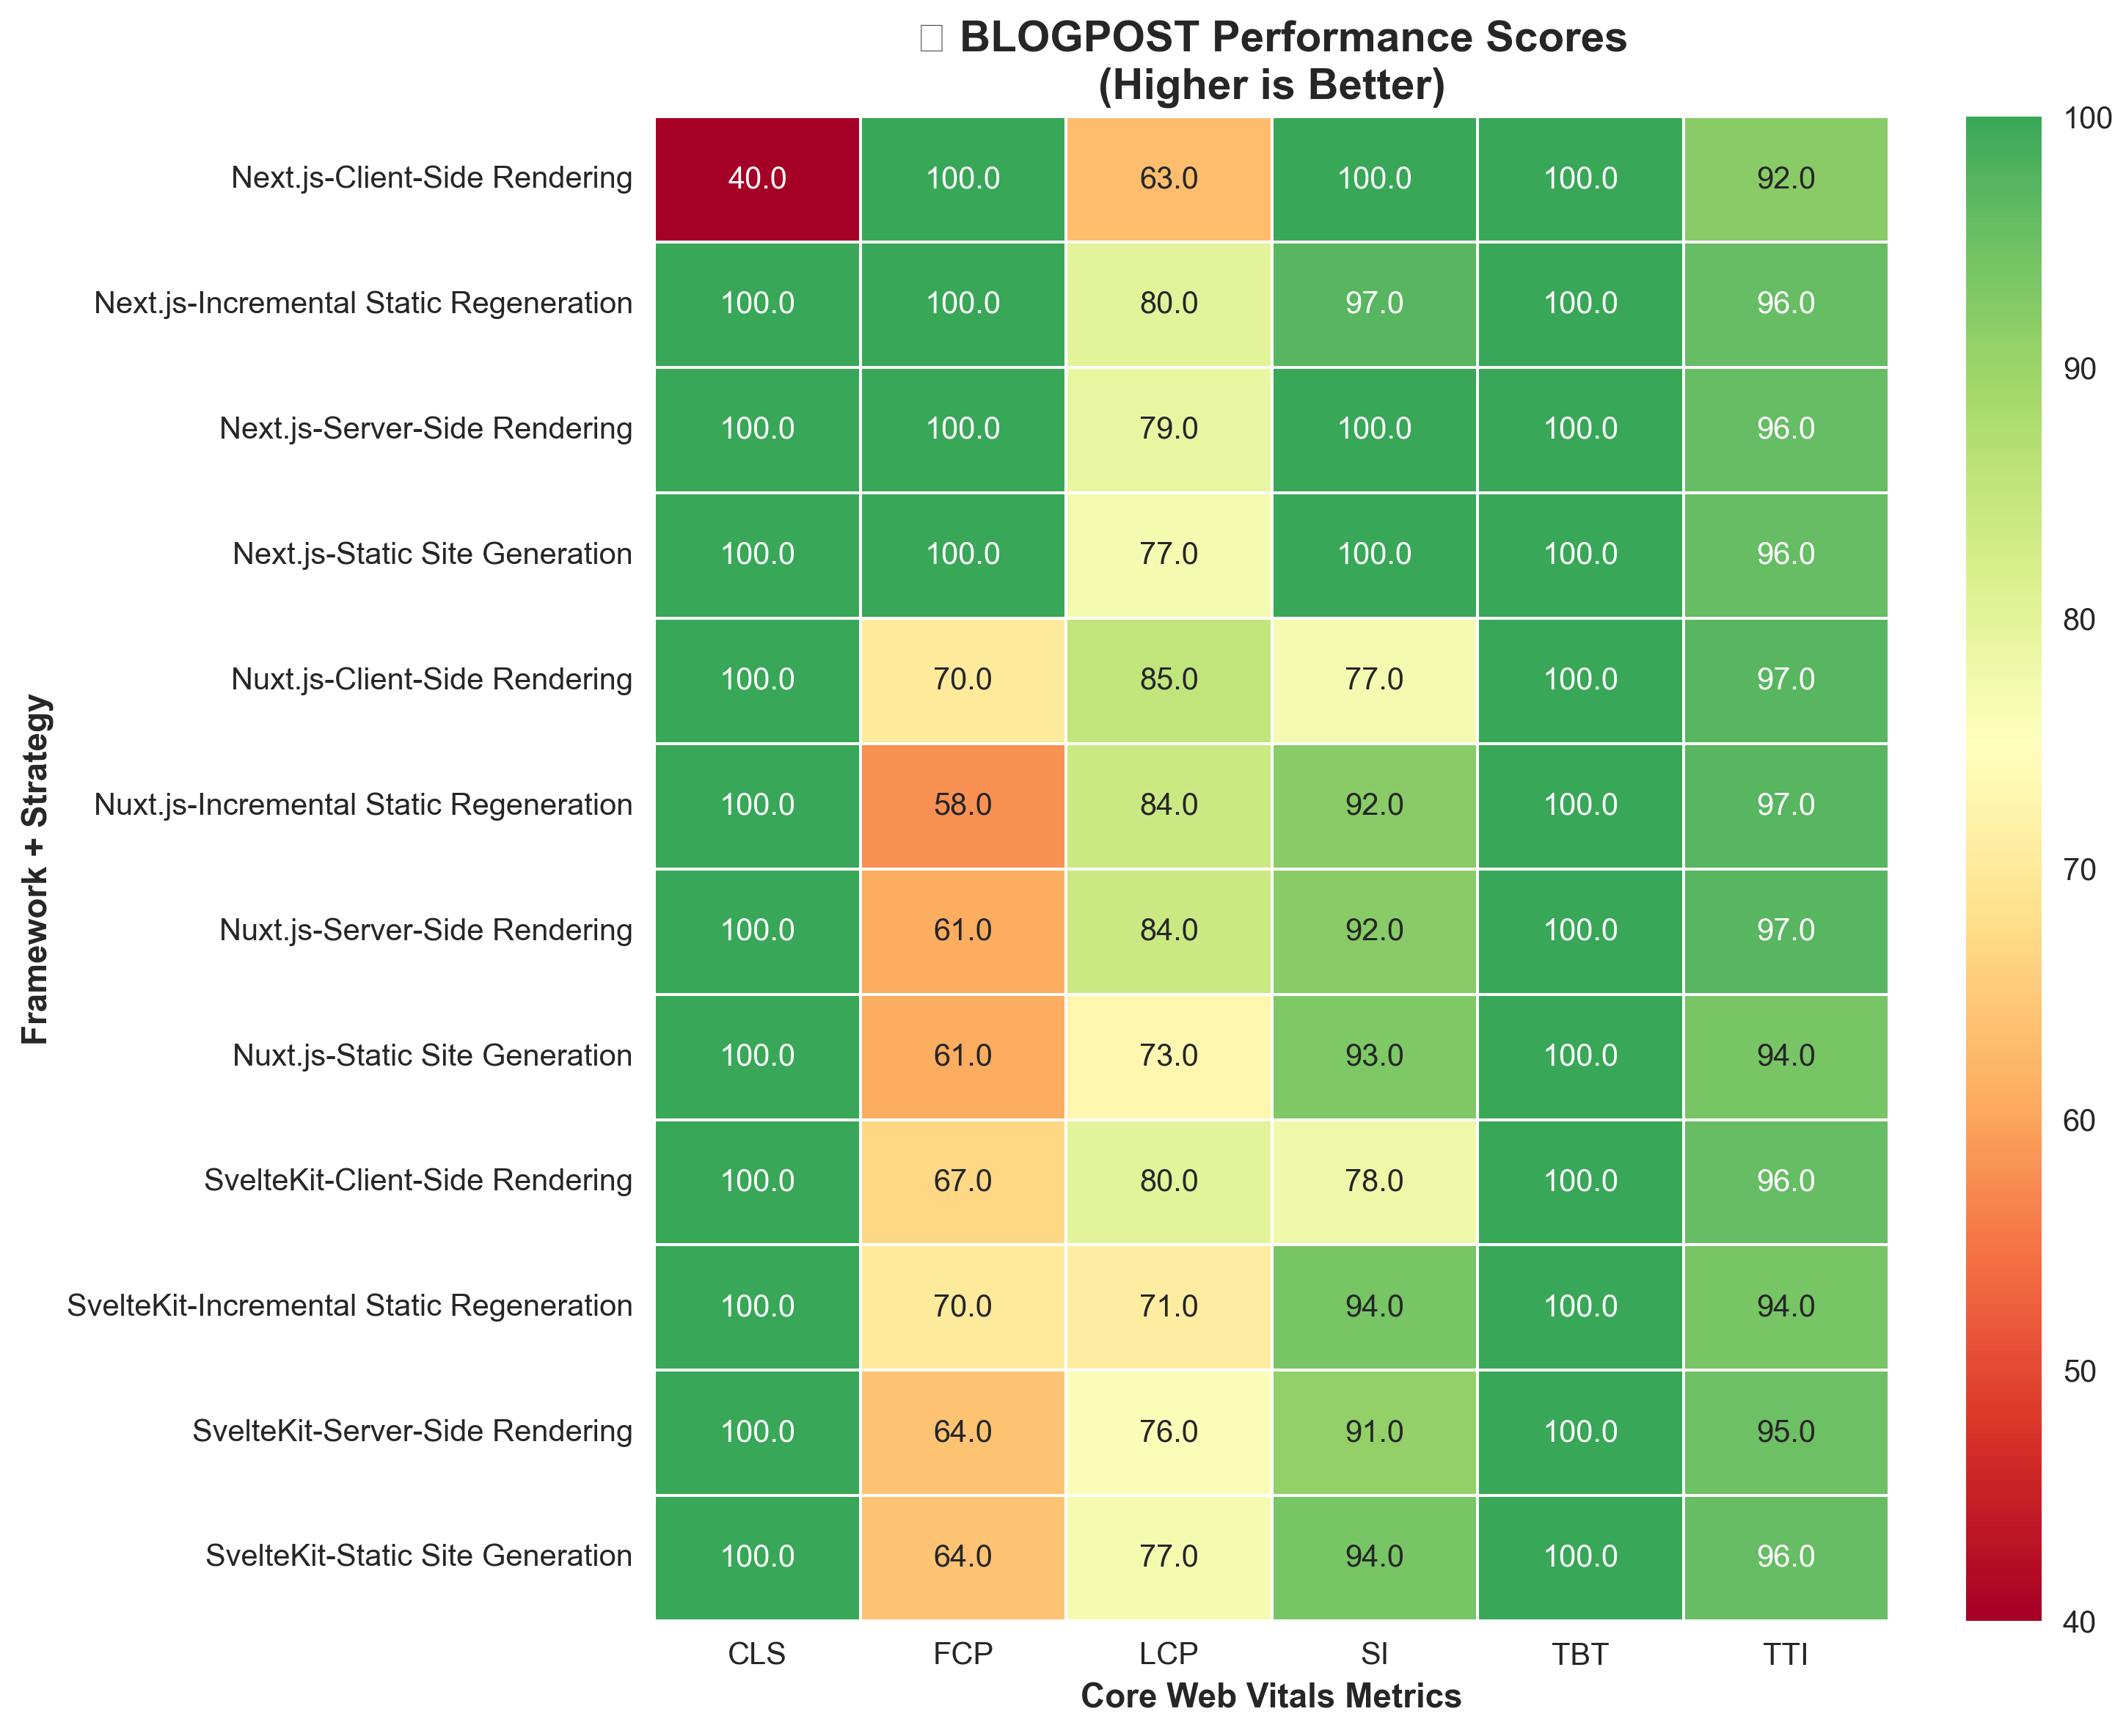
\includegraphics[width=\textwidth]{slike/rezultati/blog-post/blogPost_performance_scores.png}
    \caption{Ocjene radnih značajki - postotak (stranica pojedinog bloga) }
    \label{fig:testiranje-blog-post-postotak}
\end{figure}

\begin{figure}[H]
    \centering
    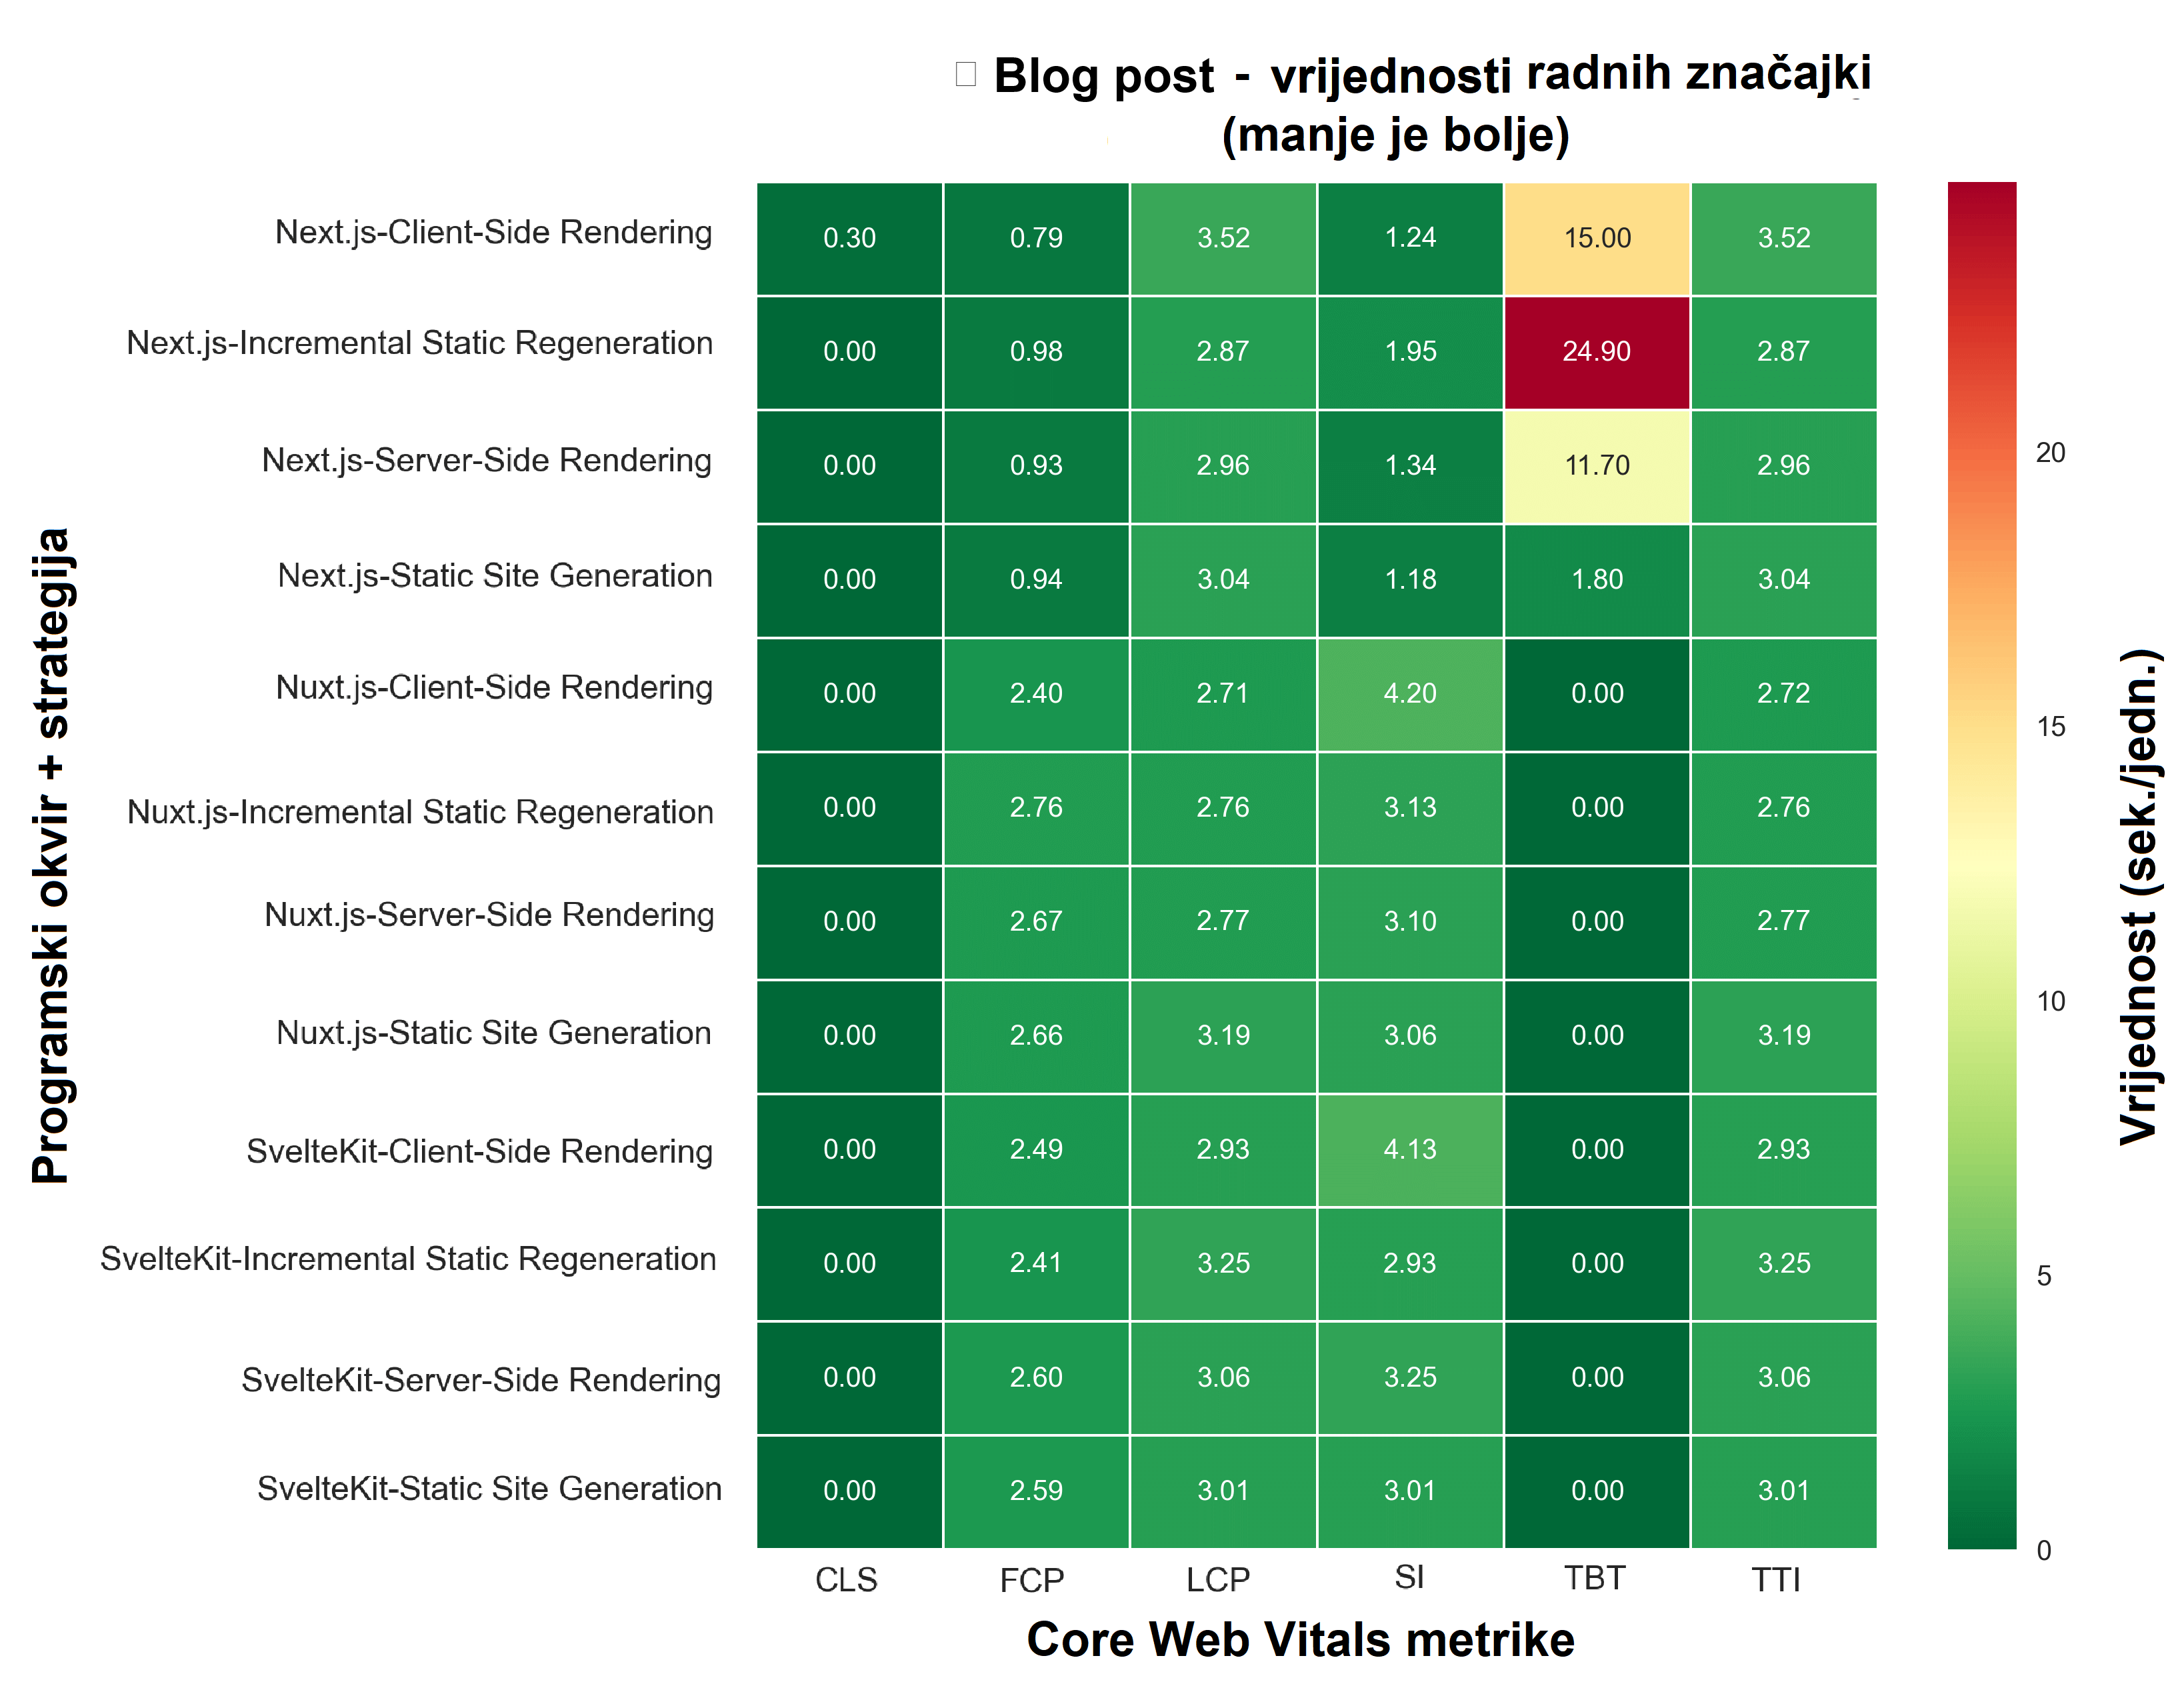
\includegraphics[width=\textwidth]{slike/rezultati/blog-post/blogPost_performance_values.png}
    \caption{Ocjene radnih značajki - vrijednosti (stranica pojedinog bloga) }
    \label{fig:testiranje-blog-post-vrijednosti}
\end{figure}

\begin{figure}[H]
    \centering
    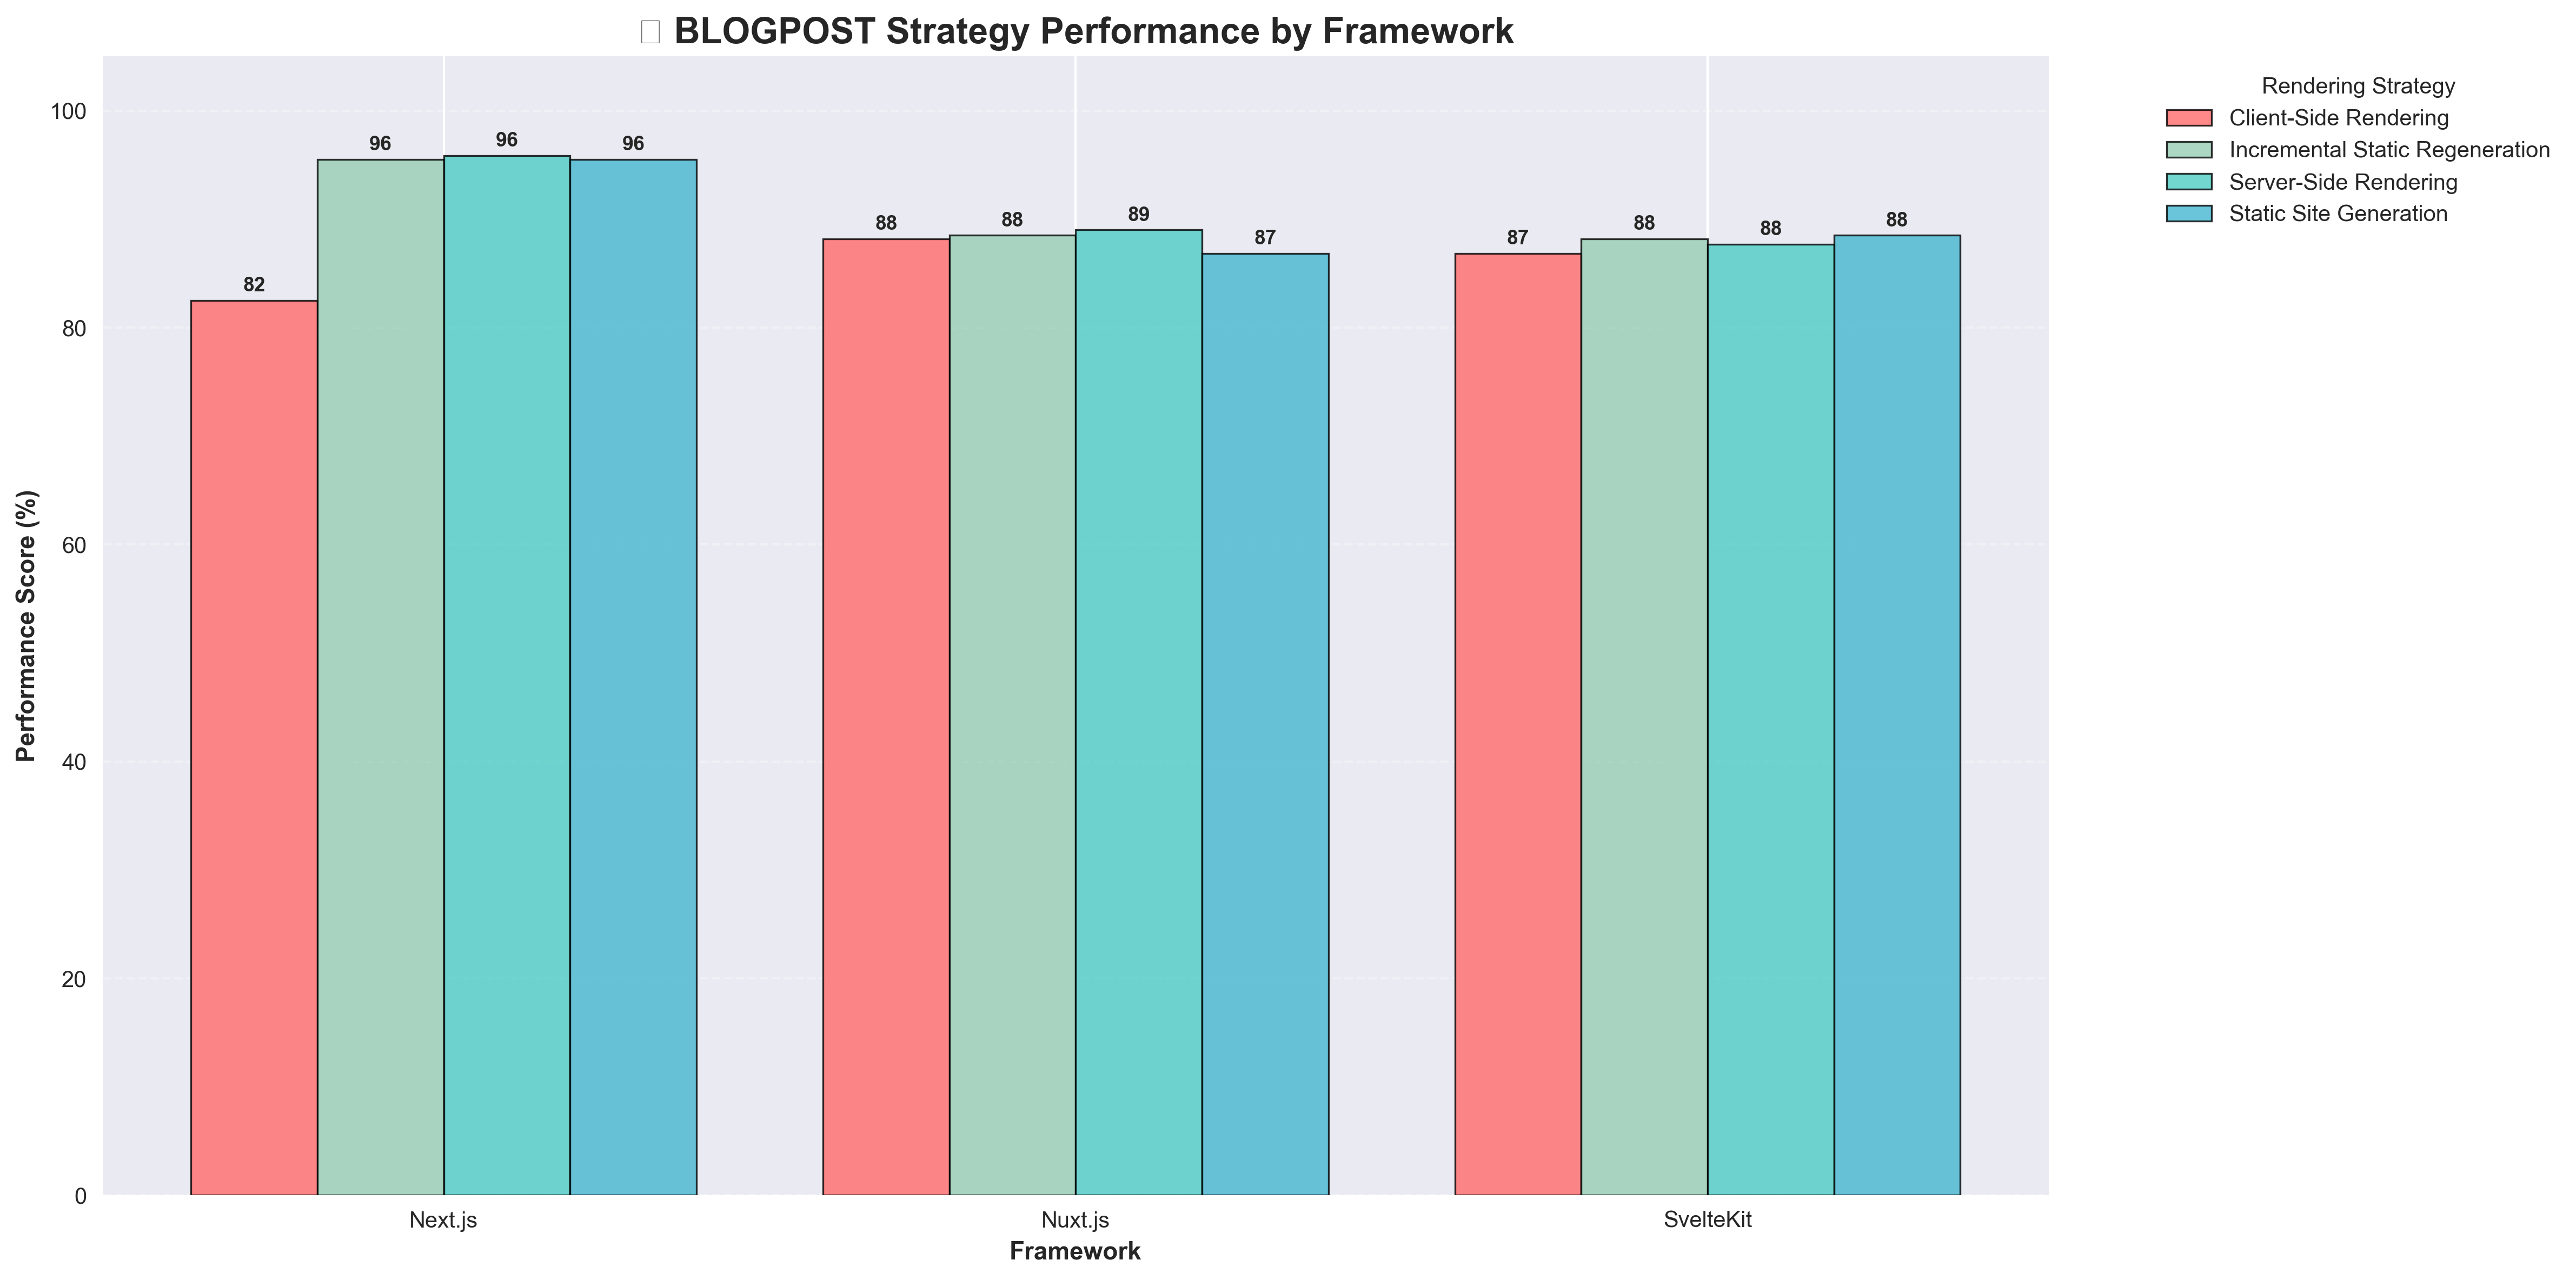
\includegraphics[width=\textwidth]{slike/rezultati/blog-post/blogPost_strategy_comparison.png}
    \caption{Ocjene radnih značajki - usporedba strategija (stranica pojedinog bloga) }
    \label{fig:testiranje-blog-post-usporedba-strategija}
\end{figure}

\newpage
\subsection{Rangiranje programskih okvira}
\begin{enumerate}
    \item Next.js: 92.3\%
    \item Nuxt.js: 88.1\%
    \item SvelteKit: 87.8\%
\end{enumerate}

\subsection{Rangiranje strategija iscrtavanja}
\begin{enumerate}
    \item Server-Side Rendering: 90.8\%
    \item Incremental Static Regeneration: 90.7\%
    \item Static Site Generation: 90.3\%
    \item Client-Side Rendering: 85.8\%
\end{enumerate}

\subsection{Najbolje kombinacije}
\begin{enumerate}
    \item Next.js + Server-Side Rendering: 95.8\%
    \item Next.js + Incremental Static Regeneration: 95.5\%
    \item Next.js + Static Site Generation: 95.5\%
    \item Nuxt.js + Server-Side Rendering: 89.0\%
    \item SvelteKit + Static Site Generation: 88.5\%
\end{enumerate}

\subsection{Vodeći po metrici}
\begin{itemize}
    \item FCP: Next.js + Client-Side Rendering (100.0\%, 0.790)
    \item LCP: Nuxt.js + Client-Side Rendering (85.0\%, 2.710)
    \item SI: Next.js + Client-Side Rendering (100.0\%, 1.240)
    \item TTI: Nuxt.js + Client-Side Rendering (97.0\%, 2.720)
    \item TBT: Next.js + Client-Side Rendering (100.0\%, 15.000)
    \item CLS: Nuxt.js + Client-Side Rendering (100.0\%, 0.000)
\end{itemize}


\newpage

\section{Zaključak}

Lorem ipsum dolor sit amet, consectetur adipiscing elit, sed do eiusmod tempor incididunt ut labore et dolore magna aliqua. Ut enim ad minim veniam, quis nostrud exercitation ullamco laboris nisi ut aliquip ex ea commodo consequat. 

\newpage

\bibliographystyle{unsrt}
\bibliography{literatura}
\newpage

%Automatski generira listu svih slika
\listoffigures
\newpage

%Automatski generira listu svih tablica
\listoftables
\newpage


\end{document}
